%%-----------------------------------------------------------------------
% Loading the packages and classes
%%-----------------------------------------------------------------------

\documentclass[12pt,twoside,a4paper,final]{book}%
\usepackage{a4}%                        %% Verwendet mehr Platz auf einer A4 Seite als Option a4paper in book
\usepackage[english,ngerman]{babel}%    %% Babel Sprachen
\usepackage[latin1]{inputenc}%          %% input encoder f�r umlaute usw.
\usepackage[T1]{fontenc}
\usepackage{amssymb}%                   %% AMS Symbole
\usepackage{amsmath}%                   %% AMS Math Funktionen
\usepackage{amsfonts}%
\usepackage[Sonny]{fncychap}%           %% Chapter Style
\usepackage[english,noprefix]{nomencl}%  %% Nomenclature (Symbolverzeichnis)
\usepackage{makeidx}%                   %% Index
\usepackage{graphicx}%                  %% Graphiken
%\usepackage[acronym]{glossaries}
\graphicspath{{img/}}
\DeclareGraphicsExtensions{.pdf,.jpeg,.png,.jpg}
\usepackage{psfrag}%                    %% Tex-Schriftarten und Formeln in EPS-Grafiken
\usepackage{color}
\usepackage{nicefrac}
\usepackage{ifthen}
\usepackage{fancyhdr}
\usepackage{subfigure}
%\usepackage[xindy, acronym, toc]{glossaries}
\usepackage{cite}
\usepackage{listings}
\usepackage{color}
\usepackage[dvipsnames]{xcolor}
\usepackage{rotating}
\usepackage{multirow}
\usepackage{eurosym}
\usepackage{capt-of}
\usepackage{glossaries}
\usepackage[ampersand]{easylist}

%Define Acronyms like
% use on every place in your document \gls{mas} for TGM or - for plural - use \glspl for TGMs
% at the first usage of this, the acronym will be introduced, everywhere else it will only be the in the short form: ``Technologisches Gewerbemuseum (TGM)''
% TIPP: USE THIS FOR EVERY NAME/SOFTWARE-TOOL/MAIN PART OF YOUR WORK, like JAVA, - so that, e.g. JAVA is not written Java everywhere else in your thesis.

\newacronym{tgm}{TGM}{Technologisches Gewerbemuseum}
\newacronym{fp}{FP-Analyse}{Function-Point-Analyse}
\newacronym{pm}{PM}{Personenmonate}

\newacronym{ma}{MA}{Moving Average}
\newacronym{sma}{SMA}{Simple Moving Average}
\newacronym{lwma}{LWMA}{Linear Weighted Moving Average}
\newacronym{wma}{WMA}{Linear Weighted Moving Average}
\newacronym{ema}{EMA}{Exponential Moving Average}
\newacronym{ama}{AMA}{Adaptive Moving Average}
\newacronym{tma}{TMA}{Triangular Moving Average}
\newacronym{er}{ER}{Efficiency Ratio}
\newacronym{dema}{DEMA}{Double Exponential Moving Average}
\newacronym{tema}{TEMA}{Triple Exponential Moving Average}
\newacronym{adx}{ADX}{Average Directional Movement Index}
\newacronym{sf}{SF}{Smoothing Factor}
\newacronym{macd}{MACD}{Moving Average Convergence/Divergence}
\newacronym{cci}{CCI}{Commodity Channel Index}
\newacronym{rsi}{RSI}{Relative Strength Indicator}

\newacronym{forex}{FOREX}{Foreign Exchange Market}
\newacronym{hft}{HFT}{High Frequency Trading}

\newacronym{bts}{BTS}{Backtesting-Software}
\newacronym{git}{GIT}{GIT-Server}
\newacronym{ide}{IDE}{Integrated Development Environment}
\newacronym{mql5}{MQL5}{MetaQuotes Language 5}
\newacronym{gui}{GUI}{Graphical User Interface}
\newacronym{dll}{DLL}{Dynamic Link Library}
\newacronym{xml}{XML}{eXtensible Markup Language}
\newacronym{xaml}{XAML}{eXtensible Application Markup Language}
\newacronym{clr}{CLR}{Common Language Runtime}
\newacronym{cls}{CLS}{Common Language Specification}
\newacronym{wpf}{WPF}{Windows Presentation Foundation}
\newacronym{jvm}{JVM}{Java Virtual Machine}
\newacronym{api}{API}{Application Programming Interface}
\newacronym{mvvm}{MVVM}{Model View Viewmodel}
\newacronym{soap}{SOAP}{Simple Object Access Protocol}
\newacronym{linq}{LINQ}{Language Integrated Query}
\newacronym{sql}{SQL}{Structured Query Language}
\newacronym{csv}{CSV}{Comma-separated values}

\newacronym{afa}{AFA}{Abschreibung f�r Abnutzung}
%%-----------------------------------------------------------------------
% Using the Hyperref-Package for PDF-Online Version
%%-----------------------------------------------------------------------

\def\usehyperref{1}

\ifnum\usehyperref=1
\usepackage[pdftex=true,
  pdftitle={Diplomarbeit},
  pdfauthor={Gottfried Koppensteiner},
  bookmarksopen,
  colorlinks,
  citecolor=blue,
  linkcolor=blue,
  breaklinks%
]{hyperref}%
\fi



%%-----------------------------------------------------------------------
% Rearranging Nomenclature
%%-----------------------------------------------------------------------


\renewcommand{\nomname}{List of symbols}
%\renewcommand{\nompreamble}{The following list only contains symbols
%  that are used continuously throughout the text. Local symbols are
%  not listed.}
\renewcommand{\nomgroup}[1]{
 \ifthenelse{\equal{#1}{A}}{\item[\textbf{General symbols}\bigskip]}{
 \ifthenelse{\equal{#1}{B}}{\item[\bigskip\bigskip\textbf{Chapter 2}\bigskip]}{
 \ifthenelse{\equal{#1}{C}}{\item[\bigskip\bigskip\textbf{Chapter 3}\bigskip]}{
 \ifthenelse{\equal{#1}{D}}{\item[\bigskip\bigskip\textbf{Chapter 4}\bigskip]}{
 \ifthenelse{\equal{#1}{E}}{\item[\bigskip\bigskip\textbf{Chapter 5}\bigskip]}{
 \ifthenelse{\equal{#1}{F}}{\item[\bigskip\bigskip\textbf{Appendix}\bigskip]}{
 }}}}}}}
\makenomenclature



%%-----------------------------------------------------------------------
% Makes Bibliography available in Winedt
%%-----------------------------------------------------------------------

%GATHER{bib_kiefer.bib}


%%-----------------------------------------------------------------------
% Definition of possible environments
%%-----------------------------------------------------------------------

\newtheorem{theorem}{Theorem}[chapter]
\newtheorem{acknowledgement}{Acknowledgement}[chapter]
\newtheorem{algorithm}{Algorithm}[chapter]
\newtheorem{axiom}{Axiom}[chapter]
\newtheorem{case}{Case}[chapter]
\newtheorem{claim}{Claim}[chapter]
\newtheorem{conclusion}{Conclusion}[chapter]
\newtheorem{condition}{Condition}[chapter]
\newtheorem{conjecture}{Conjecture}[chapter]
\newtheorem{corollary}{Corollary}[chapter]
\newtheorem{criterion}{Criterion}[chapter]
\newtheorem{definition}{Definition}[chapter]
\newtheorem{example}{Example}[chapter]
\newtheorem{exercise}{Exercise}[chapter]
\newtheorem{lemma}{Lemma}[chapter]
\newtheorem{notation}{Notation}[chapter]
\newtheorem{problem}{Problem}[chapter]
\newtheorem{proposition}{Proposition}[chapter]
\newtheorem{remark}{Remark}[chapter]
\newtheorem{solution}{Solution}[chapter]
\newtheorem{summary}{Summary}[chapter]
\newenvironment{proof}[1][Proof]{\noindent\textbf{#1.} }{\ \rule{0.5em}{0.5em}}

\renewcommand{\chaptermark}[1]{\markboth{\thechapter.\ #1}{}}
\renewcommand{\sectionmark}[1]{\markright{\thesection.\ #1}}




%%-----------------------------------------------------------------------
% Marking of overfull boxes and increasing of tolerances
%%-----------------------------------------------------------------------

% F�r die Final-Version die n�chste Zeile auskommentieren um schawarze Balken (TU-Logo im Titelblatt) zu ignorieren!
\overfullrule=10pt%                     %% Markiert �berf�llte Boxen. z.b. hbox overfull (Evtl. nicht im pdf sichtbar!!!!)
\hfuzz=1pt%                             %% Toleranz bei hbox overfull erh�ht 1pt entspr. ca. 1/3 mm


%%-----------------------------------------------------------------------
% Counter
%%-----------------------------------------------------------------------


\setcounter{secnumdepth}{3}%
\setcounter{tocdepth}{3}%



% Clear Header Style on the Last Empty Odd pages
\makeatletter
\def\cleardoublepage{\clearpage\if@twoside \ifodd\c@page\else%
    \hbox{}%
    \thispagestyle{empty}%              % Empty header styles
    \newpage%
    \if@twocolumn\hbox{}\newpage\fi\fi\fi}
\makeatother

%%-----------------------------------------------------------------------
% Avoid indents
%%-----------------------------------------------------------------------

\setlength{\parindent}{0pt}

%%-----------------------------------------------------------------------
%% Hyphenation for german abstract
%%-----------------------------------------------------------------------

\hyphenation{Fa-mi-lie
             Ski-bil-dung
             Ar-beits-wal-ze
             neg-lec-ted
             se-par-ate
             di-men-sio-nal
             her-r\"uhren
             N\"a-herungs-l\"os-ungen
             wissen-schaft-licher
             Regelungs-technik
             re-con-fi-gur-abili-ty
             manage-ment
             manu-facturing
             not-wendigen
             }


% Define F-Sharp lstlisting
\definecolor{bluekeywords}{rgb}{0.13,0.13,1}
\definecolor{greencomments}{rgb}{0,0.5,0}
\definecolor{turqusnumbers}{rgb}{0.17,0.57,0.69}
\definecolor{redstrings}{rgb}{0.5,0,0}

\lstdefinelanguage{FSharp}
                {morekeywords={let, new, match, with, rec, open, module, namespace, type, of, member, and, for, in, do, begin, end, fun, function, try, mutable, if, then, else},
    keywordstyle=\color{bluekeywords},
    sensitive=false,
    morecomment=[l][\color{greencomments}]{///},
    morecomment=[l][\color{greencomments}]{//},
    morecomment=[s][\color{greencomments}]{{(*}{*)}},
    morestring=[b]",
    stringstyle=\color{redstrings}
    }

%%-----------------------------------------------------------------------
% Colored grafix
% 1 = color
% 0 = grey
%%-----------------------------------------------------------------------


\def\colorsw{1}

%%-----------------------------------------------------------------------
% Additional remarks
% 1 = with remarks
% 0 = without remarks
%%-----------------------------------------------------------------------


\def\addnotes{0}


%%-----------------------------------------------------------------------
% Define month
%%-----------------------------------------------------------------------

\def\monthdis{Oktober 2012}

\makeglossaries
%%-----------------------------------------------------------------------
% Document
%%-----------------------------------------------------------------------


\begin{document}%
\selectlanguage{ngerman}%
\renewcommand{\indexname}{Index}%
\topmargin15.0mm


\def\tpdefault{{\sf \center \vspace*{-4cm}
%\begin{center}
%\hspace*{-1.3cm}
%\rule{17cm}{0.02cm}
%\end{center}


\begin{figure}[h]
\begin{flushright}	
		
\includegraphics[width=0.3\textwidth]{graphics/title/tgmlogo2.png}
	\label{fig:tgmlogo}
\end{flushright}
\end{figure}


\vspace{2cm}


{\Large %\bf 
DIPLOMARBEIT\\ \vspace{0.7cm}}
 {\LARGE \sloppy
{\bf \sf  \textbf{NOCTUA \\}
Wertpapierhandelsalgorithmus\\
\&\\
Performanceanalysesoftware
\\}}
%
%
\vspace*{2cm}
{\normalsize Ausgef\"uhrt in Zuge der Reife und Diplompr\"ufung\\
Ausbildungszweig Systemtechnik/Medientechnik\\ %unzutreffendes streichen
  \vspace{1.5cm}
  \normalsize unter der Leitung von\\
  \large Prof.\ Mag.\ Hans Brabenetz\\
  \normalsize Abteilung f�r
  Informationstechnologie\\
  \vspace{1.5cm}
  eingereicht am  Technologischen Gewerbemuseum Wien\\
  H\"ohere Technische Lehr- und Versuchsanstalt\\
  Wexstrasse 19-23, A-1200 Wien\\
  }}}


\begin{titlepage}
	\tpdefault
	{\sf \center \vspace{1.0cm}
	\normalsize von\\
	\large 
	Peer Nagy 5CHITI\\
	Gabriel Pawlowsky, 5BHITS\\
	Josef Sochovsky, 5BHITS\\
	\vspace {2 cm}
	\bf \sf {Wien, im \monthdis} \\
		%	\vspace{2cm}
	%	\rule{\textwidth}{0.01cm}
	
	}



	\end{titlepage}

%\begin{titlepage}
%	{\color{white}.}
%	\bigskip
%	\vspace{14cm}
%	%\vfill%
%	\noindent%
%
%	Abteilungsvorst\"andin:\hfill Prof. Dipl.-Ing. Grete Kugler\\
%	\bigskip
%	\bigskip
%
%	Termine der Reifepr�fung:\hfill 13 / 14.06.2013\\
%	\hfill 17.06.2013\\
%	\bigskip
%	\bigskip
%	
%	Pr�fungsvorsitzende:\hfill
%	Univ.--Prof.~Dipl.-Ing.~Dr.techn.~xxx\\
%	\smallskip
%
%	Erster Gutachter:\hfill Prof.\ Mag.\ Hans Brabenetz\\
%	\smallskip
%
%	Zweiter Gutachter:\hfill Prof.\ Dr.\ Helmut Vana\\
%		\smallskip
%\end{titlepage}

\frontmatter%   %% front matter will be numbered in small Roman letters

%%-----------------------------------------------------------------------


%TCIDATA{OutputFilter=latex2.dll}
%TCIDATA{Version=5.00.0.2552}
%TCIDATA{LaTeXparent=0,0,Dissertation_SW.tex}


\chapter*{Vorwort}

Diese Arbeit wurde im Jahr 2012 im Zuge unserer Ausbildung in der Abteilung f�r Informationstechnologie am \gls{tgm}, HTBLVA Wien 20, durchgef�hrt. 


\bigskip

Dankesworte

\bigskip
\bigskip
\bigskip
\bigskip



Wien, im \monthdis \hfill Name, Name, Name, Name \vfill
%
\selectlanguage{english}%
\chapter*{Abstract}

This is the english abstract.%
\selectlanguage{ngerman}%
\chapter*{Kurzfassung}

Deutsche Kurzfassung kommt hierher%


%%-----------------------------------------------------------------------
% Define Header for Content chapter
%%-----------------------------------------------------------------------


\makeatletter
\def\tableofcontents{\chapter*{\contentsname\@mkboth{\contentsname}{\contentsname}}
  \@starttoc{toc}}
\makeatother

\clearpage%
\tableofcontents
\clearpage
\listoffigures
\clearpage
\lstlistoflistings %\listoftables
\clearpage 
\markboth{Contents}{Contents}


%\addcontentsline{toc}{chapter}{\numberline{}\listfigurename}%
%\listoffigures
%\listoftables%
%\addcontentsline{toc}{chapter}{\numberline{}\listtablename}%
\clearpage%




\mainmatter%   %% main part will be numbered in Arabic letter


% include chapters
% Chapter1
\chapter{Einf�hrung} \label{chapter:einfuehrung}

\section{Hintergrund} \label{section:hintergrund}

Der Handel mit Wertpapieren ist in den letzten Jahrzehnten zunehmend systematisiert
und automatisiert worden. Kaum jemand trifft Handelsentscheidungen ohne fundierte Analyse leichtfertig aus dem Bauch
heraus. Diese Analyse unterwirft sich aber damit einem programmatischen
Schema, das ebenso gut auch automatisch angewandt werden kann: trifft eine Person
Entscheidungen nach einem spezifischen Schema, kann ein Computer dies ebenso und sogar
schneller und genauer.\\

Schon seit einiger Zeit sind Computerprogramme auf dem Vormarsch, die algorithmische Kauf- und Verkaufsauftr�ge an der B�rse durchf�hren.
Daf�r kommen diverse  Algorithmen zur Einsch�tzung zuk�nftiger Kurswerte zum Einsatz.
Besonders gut geeignet daf�r scheint die Technische Analyse, z.B. Verfahren die Trendbestimmung und
des Trendfolgens. Auch wenn es reichlich Kritik an solchen Systemen gibt, werden sie von
sehr viele Marktteilnehmer angewandt. Das f�hrt aber zumindest teilweise zu einer
selbsterf�llenden Prophezeiung, da sich die Kurse durch das Verhalten der Mehrheit der Marktteilnehmer bilden.
Computer helfen dabei, komplizierte Berechnungen in k�rzester Zeit durchzuf�hren und in vielen F�llen Entscheidungen aus Handelssystemen
ohne manuellen Eingriff schnell umzusetzen. \cite{bank_hochfrequenz}

Ein weiterer Vorteil des algorithmischen Trading sind die Geschwindigkeit und die Genauigkeit, mit
der Computer arbeiten k�nnen, an die Menschen nicht heranreichen. Durch systematische und
statistische Entscheidungen k�nnen menschliche Emotionen aus dem Spiel gelassen und dadurch
auch das Risiko besser abgesch�tzt werden.\\

Solche Algorithmen sollten w�hrend der Entwicklung und besonders vor produktivem Einsatz ausreichend evaluiert und getestet werden,
was sich als kompliziert erweisen kann, da f�r verschiedene Zeitr�ume und Kurse getestet werden sollte. Da vergangene Resultate sich nicht
umbedingt in der Zukunft wiederholen m�ssen, ist es besonders wichtig, dass Algorithmen mit vielen unterschiedlichen historischen Daten
getestet werden.\\

Die Informationsflut, die schon f�r Aktien existiert, ist l�ngst nicht mehr manuell zu
bew�ltigen. R�ume voller Server rechnen ununterbrochen mit den Kursdaten und versuchen jeden
m�glichen Vorteil auszunutzen, um den Gewinn zu optimieren. Die verwendeten Modelle, Ans�tze
und Algorithmen werden in der Regel geheim gehalten, da viel Geld von den Entscheidungen der
Software abh�ngt. W�ren verwendete Algorithmen publik, w�rden diese nicht mehr lange profitabel
funktionieren. Daher bleiben die Vorgangsweisen, die besser funktionieren und gro�en Unternehmen
reale Gewinne einbringen, geheim. Im Internet und einschl�giger Literatur l�sst sich einiges zu verschiedenen Ans�tzen
finden, wie mit vorhandenen Daten Handelsentscheidungen berechnet werden k�nnen.
Solche Strategien lassen sich zwar problemlos finden, ein objektiver Vergleich ist aber entweder sehr umst�ndlich oder gar nicht m�glich.\\

\section{Motivation} \label{section:motivation}

F�r ein automatisiertes Handeln mit Wertpapieren an der B�rse soll ein Algorithmus
entwickelt werden, der die optimalen Handelsentscheidungen berechnet. Damit man den
Algorithmus sowohl w�hrend der Entwicklung, als auch in finaler Form,
hinsichtlich der Performance evaluieren kann, soll au�erdem eine Software
implementiert werden, die automatisch mit historischen Daten, also bereits vergangenen Bewegungen
an der B�rse, rechnet und eine vern�nftige Testumgebung darstellt.\\

Das Projekt Noctua hat somit zwei grundlegende Aufgaben. Die Entwicklung eines Handelsalgorithmus
und einer \gls{bts}, die es erm�glicht ebensolche Algorithmen zu evaluieren.  
 
\begin{itemize}
	\item Der Algorithmus soll dabei Trends m�glichst fr�h identifizieren und diesen solange folgen
				bis sie ihre Nachhaltigkeit verlieren. Au�erdem soll er auf �ndernde Bedingungen
				m�glichst flexibel reagieren und die Strategie dementsprechend anpassen.
				Die Programmierung muss dabei ausreichend performant sein, damit die Ausf�hrungsgeschwindigkeit
				auf einem modernen Computersystem in Echtzeit m�glich ist. 
	\item Damit die Handels-Performance auch �ber mehrere Versionen des Algorithmus hinweg verglichen
				werden kann, soll eine \gls{bts} entwickelt werden. Diese soll mithilfe
				von historischen Daten funktionieren. Dieses Programm simuliert einen rapiden Ablauf
				von m�glicherweise mehreren Jahren B�rsengeschichte, die den Rechenablauf mit
				verschiedenen Marktzust�nden und Marktzustands�nderungen konfrontiert. Die
				Ergebnisse dieser Simulation k�nnen dann ausgelesen werden, um sie mit den
				vorherigen Ergebnissen auf eine etwaige Steigerung oder auch einen Abfall der
				Performance zu analysieren. Damit man einen reibungslosen Austausch der
				verschiedenen selbst entwickelten Rechenmodulen, aber auch der vorhandenen
				Standardalgorithmen anbieten kann, muss daf�r gesorgt werden, dass das simple und
				effiziente Austauschen des momentan verwendeten Algorithmus erm�glicht wird.
\end{itemize}

Noctua hat die Aufgabe durch die \gls{bts} eine benutzerfreundliche M�glichkeit zu schaffen,
programmierte Handelsstrategien gegen reale vergangene Kurse zu evaluieren und so den
Entwicklungsprozess zu vereinfachen und zu verk�rzen.

Die Entwicklung eines eigenen Algorithmus, der Methoden der Technischen Analyse implementiert,
soll au�erdem h�ufige Behauptungen zu g�nstigen Handelsstrategien auf den Pr�fstand stellen
und herausfinden, ob mit einfachen Mitteln profitable Strategien umsetzbar sind.
%
%% !TeX root = ../../Noctua_Diplomarbeit.tex
% Chapter2

\chapter{Machbarkeitsstudie} \label{chapter:machbarkeitsstudie}

% !TeX root = ../../Noctua_Diplomarbeit.tex

\section{Einleitung}

\label{section:einleitung}

Das algorithmische Handeln hat besonders in den letzten zwei Jahrzehnten rasant zugenommen. 2011 wurde davon ausgegangen, dass mindestens 30\% des Aktienhandelsvolumen in den USA bereits algorithmischer Natur ist. Alleine schon die Kommissionen der Broker f�r algorithmisch abgewickelte Entscheidungen beziehen sich weltweit auf etwa \textdollar{400-600} Millionen. Die meisten der verwendeten Algorithmen sind allerdings propriet�rer Natur und dienen h�ufig nicht der direkten Optimierung des Profits, sondern dem Aufteilen gro�er Orders und der Minimierung des Risikos und der Kosten. \cite{avellaneda-algorithmic-2011}\\
	Algorithmen, die direkt Handelsentscheidungen treffen, existieren ebenfalls und werden h�ufig f�r Fonds eingesetzt, die an Privatpersonen weiterverkauft werden. Besonders kleinere Unternehmen und Privatpersonen haben nicht die Kapazit�ten, um beim \gls{hft}, wo jede Millisekunde z�hlen kann, mitzumischen. Klassische Handelssysteme k�nnen allerdings sehr wohl als Computersoftware umgesetzt werden und bieten die Vorteile nach einem klar definierten System schneller Entscheidungen zu treffen und dies gegebenenfalls auch ohne menschliche Aufsicht.\\
	M�rkte, und insbesondere Aktienm�rkte, verhalten sich nicht immer invariant, sondern k�nnen ihre intrinsischen Systematiken mit der Zeit �ndern. Folglich kann es zu Einbu�en bei der Performance von Algorithmen kommen, die ebendiese Systematiken ausnutzen. Um dies zu verhindern oder zumindest die Effekte zu vermindern, muss ein erfolgreicher Algorithmus eine gewisse Adaption bzw. eine Anpassung und dadurch zus�tzliche Flexibilit�t der Parameter erm�glichen.
	Ziel des Projektes ist es, genau solch ein System zu entwickeln und umzusetzen. Die vollst�ndige Eigenentwicklung erm�glicht volle Einsicht in alle relevanten Bereiche des Algorithmus und der verwendeten Parameter. Au�erdem kann mithilfe einer zu entwickelnden \gls{bts} die Performance des Algorithmus anhand diverser Kriterien gezielt gemessen werden.
	Im folgenden geht es nun darum, zu kl�ren, welche Ans�tze zur Umsetzung eines solchen Algorithmus m�glich sind und wie ihre technische Implementierung aussehen k�nnte. Zus�tzlich soll die optimale L�sung sowohl f�r alle Aspekte des Algorithmus als auch der \gls{bts} er�rtert werden.
\clearpage
% !TeX root = ../../Noctua_Diplomarbeit.tex

\section{Finanzwirtschaftliche Grundlagen}

\label{chapter:finanzgrundlagen}

Aufgabe dieses Kapitels ist es zun�chst ein Fundament f�r die Verst�ndnis dieser Arbeit zu legen und Funktionsweisen, Vorg�nge, sowie verschiedene Ans�tze zu erl�utern.\\

\subsection{B�rse}

Eine B�rse ist ein Handelsmarkt auf dem sich Preise durch Angebot und Nachfrage von Handelspartners bilden und Handel nicht direkt zwischen K�ufern und Verk�ufern, sondern �ber berechtigte H�ndler, abgewickelt wird. Wichtig ist dabei, dass immer f�r ausreichend Liquidit�t gesorgt werden muss, so dass jederzeit Wertpapiere gekauft und auch verkauft werden k�nnen.\\
	Handelsvorg�nge oder \emph{Trades} resultieren aus einer Erwartungshaltung der Marktteilnehmer. \cite{boerse_wien_funktion} \cite{boerse_frankfurt_funktion} 
Unter der Annahme von steigenden Kursen werden Einheiten gekauft, i.e. es wird \emph{long} gegangen, werden fallende Kurse erwartet, werden entweder existierende St�ckzahlen verkauft oder es wird sogar ein Leerverkauf get�tigt, i.e. eine \emph{short}-Position er�ffnet. Damit wird der Verkauf von geborgten Wertpapieren bezeichnet, die zu einem sp�teren Zeitpunkt beim Schlie�en der short-Position erst gekauft werden. Sinken die Kurse dazwischen wird daher zu einem h�heren Preis verkauft, als sp�ter gekauft wird und es entsteht die Differenz als Gewinn. \cite{gabler_leerverkauf}\\
	Wollen mehr Handelsteilnehmer oder \emph{Trader} kaufen, als verkaufen steigt der Preis aufgrund der hohen Nachfrage, man spricht auch von einem Bullenmarkt. \cite{duden_bullenmarkt}
Ist es andersherum so, dass die Verk�ufer �berwiegen und der Preis sinkt handelt es sich um einen B�renmarkt. \cite{duden_baerenmarkt}\\
\\

\subsubsection{Preise}

F�r jedes Wertpapier wird ein sogenanntes Orderbuch gef�hrt, das die aktuellen Kauf- und Verkaufauftr�ge beinhaltet. Investoren interessieren sich meist f�r die sogenannte Quote-Zeile, die Informationen zu den g�nstigsten Konditionen sowohl auf K�ufer-, als auch auf Verk�uferseite bietet.\\
	Eine Quote-Zeile von Apple (AAPL) k�nnte dabei folgenderma�en aussehen.

\begin{center}
\begin{tabular}{|c|c|c|c|}
\hline 
Bid & Bid Size & Ask & Ask Size \\ \hline
691.52 & 700 & 691.66 & 300 \\ \hline
\end{tabular}
\end{center}

Der Bid-Preis von \textdollar{691.52} ist das h�chste vorhandene Gebot f�r eine Apple-Aktie. Die Bid-Size gibt die Information �ber die Anzahl an Aktien, die K�ufer zu diesem Preis erstehen wollen. Die Anzahl wird in \emph{round lots} angegeben; meist entspricht ein round lot 100 St�ck der Aktie. Die Bid-Seite beschreit somit die K�uferseite.\\
Der Ask-Preis und die Ask-Size beschreibt hingegen das beste Angebot auf der Verk�uferseite. In diesem Fall werden 300 round lots f�r den St�ckpreis von \textdollar{691.66} angeboten.\\
	Soll ein Handel so schnell als m�glich abgewickelt werden muss zum Ask-Preis gekauft und zum Bid-Preis verkauft werden. In diesem Fall ver�ndert sich die Quote-Zeile so, dass der n�chstbeste Auftrag angezeigt wird. Diese Hintereinanderreihung von Angeboten wird auch als Orderbuchtiefe bezeichnet.\\
	Angenommen ein K�ufer ist nicht bereit zum aktuellen Ask-Preis zu kaufen. Er will bessere Konditionen und schickt eine \emph{Limit-Order}, d.h. zu gegebenem Preis oder besser \footnote{IB-Ordertypen siehe: http://www.interactivebrokers.com/de/p.php?f=orderTypes}, mit einem Limit, das zwischen Ask- und Bid-Preis liegt. Sein Kaufgebot ist damit h�her als der zuvor h�chste und wird daher sofort in der Quote-Zeile auf der Bid-Seite angezeigt.\\
\\
Der Aktienkurs wird mithilfe dieser vorhandenen Orders so gebildet, dass stets der h�chste Umsatz entsteht.
\cite{charttec_kursfeststellung}

\subsection{Markt}

Aktienpreise setzten sich vollst�ndig durch Angebot und Nachfrage zusammen. Nachfrage entsteht wenn Handelsteilnehmer annehmen, dass die Preise steigen, Angebot durch die Erwartung von negativen Kursver�ufen.\\
	Diese Annahmen beruhen auf einer Vielzahl von Informationen, die zur Verf�gung stehen. Somit haben diese Informationen einen direkten Einfluss auf die Aktienkurse. Ver�ffentlicht ein Unternehmen seine Bilanz und fallen darin die Gewinne h�her aus als erwartet, wird die Aktie aufgrund dieser Information steigen. Die Preise reflektieren aber nicht nur realisierte Gewinne, sondern auch potentielle zuk�nftige. W�ren in der Theorie alle m�glichen Informationen allen Handelsteilnehmern bekannt, w�rde sich der Kurs nur mehr durch das Auftauchen von neuen Informationen ver�ndern. In der Praxis verh�lt es sich anders, da weder alle Informationen vorhanden sind, noch Handelsteilnehmer absolut rational agieren.\\
Diese in den 1960ern entwickelte Theorie wird als \emph{Efficient Market Hypothesis} bezeichnet und besagt kurzgefasst, dass Marktpreise alle verf�gbaren Informationen vollst�ndig widerspiegeln.\\
	Au�er der Schlussfolgerung, dass Nachrichten und Ereignisse f�r Preisentwicklungen h�chst relevant sind, l�sst sich ebenfalls folgern, dass positive Informationen, z.B. eine Wachstumsprognose, keinen Kursanstieg bedeuten muss, weil diese schon in dem aktuellen Marktpreis inbegriffen sein kann. \cite{lo_efficient_market_hypothesis}\\
	Unter der Pr�misse, dass die Efficient Market Hypothesis uneingeschr�nkte G�ltigkeit besitzt, l�sst sich au�erdem deduzieren, dass Preise nicht vorhergesehen werden k�nnen. W�re dies n�mlich der Fall und k�nnte jeder Markteilnehmer Preise beliebig genau vorhersagen, w�re niemand bereit unter dem vorhergesagten Preis zu verkaufen und niemand w�rde dar�ber Kaufen. Daraus resultiert eine sofortiger Sprung auf den vorhergesagten Preis. Da nur neue Informationen, die \emph{noch nicht bekannt sind} das Preisniveau ver�ndern, sind folglich auch die Preise noch nicht bekannt. \cite{}
\\
Da ein Marktpreis bei erh�hter Nachfrage steigt, ist es f�r Aktienanleger sinnvoll Geld dort anzulegen, wo auch andere investieren. Gewinn liegt daher darin herauszufinden was die Mehrheit oder der Markt denkt und nicht in der pers�nlichen Einsch�tzung der Information. John Maynard Keynes beschreibt diese Theorie schon 1936 in seiner \emph{General Theory}.\\
	In dieser Theorie l�sst sich eine R�ckkopplung an Information erahnen. Nicht nur die urspr�ngliche Information selbst spielt eine Rolle, sonder auch die Reaktion darauf, im Falle von Aktien also die Kursentwicklung. Dieser iterative Prozess ben�tigt aufgrund von menschlichem Handeln aber auch seine Zeit. Dadurch entstehen durch Kursschwankungen und die verursachten Reaktionen Trendbewegungen in den M�rkten. Erst durch diesen, eigentlich psychologischen Effekt, funktionieren Charttechniken und technische Analysen.\\
	F�r jene, die sich zus�tzlich noch mit makro�konomischen Zusammenh�ngen befassen besteht trotzdem weiterhin ein Vorteil. Marktr�ckkopplungen unterliegen einem "Herdentrieb" und k�nnen zu Spekulationsblasen f�hren. �bergeordnete Vorg�nge k�nnen somit fr�hzeitige Hinweise liefern und bei der korrekten Interpretation von den resultierenden Kursverl�ufen helfen. \cite{singer_herdentrieb}

\subsubsection{Marktzust�nde}

Um die Performance von Trendfolgemethoden zu optimieren sollen verschiedene \emph{Marktzust�nde} unterschieden werden, die sich auf den Kursverlauf auswirken. Zu diesem Zweck k�nnen diverse Kriterien untersucht werden. Angefangen bei l�ngeren Trendverl�ufen, die nicht zum aktiven Handel genutzt werden, �ber W�hrungswechselkurse bis zu Zinss�tzen.\\
	Beispielsweise k�nnte sich herausstellen, dass bei einem langfristigen Aufw�rtstrend bei Kaufsignalen die long-Positionen immer gr��er ausfallen sollten, als die short-Positionen bei Verkaufssignalen oder dass erh�hte Volatilit�t und steigende Zinsen einen Kurseinbruch ank�ndigen.

\subsection{Trends und Gleitende Durchschnitte}

\subsubsection{Trends}

Bei der Trendbestimmung in B�rsenkursen gelten gleitende Durchschnitte, oder \glspl{ma}, als ein beliebtes Mittel und infolge dessen h�ufig genutzter Indikator. Die klassische Technische Analyse ist oft subjektiv und unterliegt einem gewissen Interpretationsspielraum, w�hrend \glspl{ma} f�r algorithmische Handelssysteme klare Entscheidungen generieren k�nnen.\\
	 Ein \gls{ma} ist wie das zweite Wort bereits verr�t eine Art statistischer Durschnitt von einer Reihe von Werten. \emph{Gleitend} oder \emph{moving} bedeutet, dass nicht alle historischen Daten in die Durchschnittsberechnung einflie�en, sondern nur eine beschr�nkte Anzahl der vergangenen Daten. Zur Berechnung von diversen \glspl{ma} gibt es unterschiedliche Varianten zur Wahl der verwendeten Rohdaten. Klassischerweise werden Schlusskurse zur \gls{ma}-Berechnung verwendet, wobei manche Trader es vorziehen, Open- oder Mittelwerte aus Open- und Close heranzuziehen. Eine weitere Variante ist eine separate Berechnung von \glspl{ma} f�r High- und Low-Kurse, wodurch ein Band entsteht, das einen Art Neutralbereich anzeigt, der beispielsweise als Signalfilter verwendet werden kann.\\
	Prinzipbedingt sind alle \glspl{ma} Trendfolgeindikatoren, sie antizipieren keine zuk�nftigen Kursver�nderungen, wie viele Methoden der Technischen Analyse, sondern reagieren nur auf bereits stattgefundene Trendwenden.\\

\subsubsection{Simple Moving Average}

Bei einem \gls{sma} wird f�r jeden neuen Wert jeweils aus den letzten $n$ Werten ein arithmetischer Mittelwert berechnet. Soll aus einer Reihe von Close-Kursen ein 10-Tages-\gls{sma} berechnet werden, werden dazu die letzten 10 Schlusskurse addiert und anschlie�end durch 10 dividiert um einen Wert zu erhalten. F�r den folgenden Mittelwert wird der �lteste subtrahiert, ein weiterer neuer Wert addiert und die Summe anschlie�end wieder f�r einen Mittelwert durch 10 dividiert. Auf diese Weise entsteht ein gegl�tteter Kurs, der kurzzeitige Preisver�nderungen abschw�cht, wodurch Trends klarer erkennbar werden.\\
	2 h�ufig kritisierte Eigenschaften des \gls{sma} sind, dass erstens nicht alle vorhandenen Daten in die Berechnung miteinbezogen werden und zweitens alle verwendeten Kursdaten mit gleicher Gewichtung in das Resultat eingehen. Bei einem 10-Tage-\gls{sma} hat jeder Kurswert, unabh�ngig vom Alter, eine Gewichtung von 10\%, bei einem 20-Tage-\gls{sma} 5\%.

\begin{equation}
	\label{Simple Moving Average}
	P^{*}_t = \frac{1}{n} * \sum\limits_{i=0}^n{x_{t-n}}
\end{equation}

\subsubsection{Linear Weighted Moving Average}

Um eines der Probleme des \gls{sma} zu vermeiden, und zwar die gleiche Gewichtung von allen Daten �ber die Zeit, kann ein \gls{lwma} verwendet werden. Dabei werden Daten zu fr�heren Zeitpunkten geringer gewichtet, als aktuellere Daten. Konkret wird der neueste Eintrag mit $n$ multipliziert, der davor mit $n-1$ und so weiter bis der letzte den Multiplikationsfaktor 1 erh�lt. Die daraus gebildete Summe muss anschlie�end noch durch die Summe der Multiplikatoren dividiert werden, um einen Durchschnitt zu erhalten. Bei einem 10-Tage-\gls{lwma} werden die Kursdaten von neu nach alt mit $10, 9, 8, 7,\dots, 1$ multipliziert und die anschlie�end gebildete Summe durch $10+9+8+7+\dots+1$ dividiert.

\begin{equation}
	\label{Linear Weighted Moving Average}
	P^{*}_t = \frac{\sum\limits_{i=1}^n{P_i * i}}{\sum\limits_{i=1}^n{i}}
\end{equation}

\subsubsection{Exponential Moving Average}

Der \gls{ema} versucht beide Hauptkritikpunkte am \gls{sma} zu l�sen, indem er neuere Werte immer st�rker gewichtet und alle zur Verf�gung stehenden Daten in die Berechnung miteinbezieht. Man spricht auch vom exponentiell gegl�tteten gleitenden Durchschnitt. Dazu muss ein \emph{\gls{sf}}, auch Gl�ttungsfaktor genannt, zwischen 0 und 1 gew�hlt werden mit dem der neueste Wert multipliziert wird. Der zuvorige Wert wird mit der Differenz des \gls{sf} und 1 multipliziert. Der aktuelle \gls{ema} ergibt sich dann aus der Addition dieser beiden gewichteten Werte. Dadurch bleibt jeder Kurswert unendlich lange in der zuk�nftigen Berechnung bestehen, dessen Bedeutung konvergiert aber gegen 0. Aus ebendiesem Grund handelt es sich mathematisch rigoros betrachtet bei dem \gls{ema} nicht wirklich um einen \emph{moving} average, da sich der Wertebereich nicht verschiebt, sondern immer alle Werte verwendet werden. \cite{klinker_exponential_2011}
	Dies beschreibt eine rekursive Vorgangsweise; anders w�re es auch m�glich mit dem �ltesten (bzw. zweit�ltesten) Wert zu beginnen und die Berechnung bis zum neuesten fortzusetzen.
Die folgende Formel soll die Berechnung des exponentiell gegl�tteten Preises $P^{*}_t$ zum Zeitpunkt $t$ verdeutlichen. Dabei ist $\alpha$ der \gls{sf} und $P^{*}_{t-1}$ der exponentiell gegl�ttete Preis zum Zeitpunkt $t-1$.

\begin{equation}
	\label{Exponential Moving Average}
	P^{*}_t = \alpha * P_{t} + (1 - \alpha) * P^{*}_{t-1}
\end{equation}

\cite{murphy_technische_2004}
\\
\\
Um den Lag, also das hinterherhinken hinter dem tats�chlichen Kurs zu reduzieren gibt es die M�glichkeit neue Daten noch st�rker zu gewichten, als bei einem normalen \gls{ema}.
1994 von Patrick Mulloy eingef�hrt, schaffen sowohl der \gls{dema} als auch der noch st�rker neue Daten gewichtende \gls{tema}, bei dieser Problematik Abhilfe.
Den \gls{dema} darf man sich allerdings nicht als \gls{ema} eines bereits berechneten \gls{ema} vorstellen. Das w�rde zu einer ungew�nschten starken Abwertung aktueller Daten f�hren, wie an den Gewichtungsgraphen in Abbildung \ref{wrong_dema_tema} zu sehen ist. Tats�chlich wird der \gls{dema} aus einer Zusammensetzung aus einem einfachen und einem doppelten \gls{ema} berechnet, wodurch ein neuer \gls{ma} entsteht mit weniger Lag als jede der Komponenten. \cite{mulloy_smoothing_1994}

\begin{equation}
	\label{Double Exponential Moving Average}
	DEMA = 2*EMA - EMA(EMA)
\end{equation}

\begin{equation}
	\label{Triple Exponential Moving Average}
	TEMA = 3*EMA - 3*EMA(EMA) + EMA(EMA(EMA))
\end{equation}

\begin{figure}[htbp]
	\centering
	\begin{minipage}[b]{0.4\textwidth}
		\centering
 			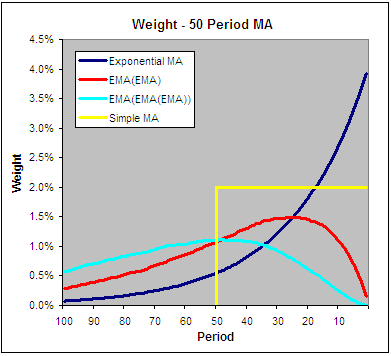
\includegraphics[width=0.9\textwidth]{graphics/chapter2/fingrundlagen/wrong_dema_tema.png}
			\caption[Falsche Multiple Exponential Average Gewichtung]{Falsche Double und Triple Exponential Average Gewichtung}
			\label{fig:wrong_dema_tema}
	\end{minipage}\hspace{0.01\textwidth}	% Abstand zwischen den Bildern = 1% der Textbreite
	\begin{minipage}[b]{0.4\textwidth}
		\centering
 			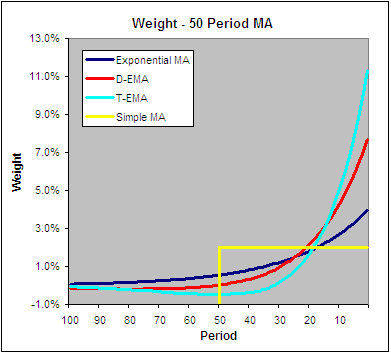
\includegraphics[width=0.9\textwidth]{graphics/chapter2/fingrundlagen/right_dema_tema.png}
			\caption[Richtige Multiple Exponential Average Gewichtung]{Richtige Double und Triple Exponential Average Gewichtung}
			\label{fig:right_dema_tema}
	\end{minipage}
\end{figure}

\cite{etf_hq_dema_tema}

\subsection{Unterst�tzung und Widerstand}

Die Kurse von Aktien unterliegen, wie bereits erw�hnt gewissen Trends, die entweder auf-, ab- oder auch seitw�rts verlaufen, wenn weder das eine, noch das andere klar feststellbar ist. Bei steigenden Kursen erreichen diese irgendwann ein Level, bei dem der Preis nicht mehr als billig angesehen wird und der Kurs dreht um. Der Trend verliert also seine Nachhaltigkeit. Dieses Level wird als \emph{Widerstand} oder \emph{Resistance} bezeichnet, da dieser nur schwer �berwunden wird. Sinkt der Kurs eine Weile wieder und sonstige Bewertungskriterien des Handelsgutes haben sich nicht signifikant ver�ndert, erreicht der Kurs einen Punkt, bei dem er wieder interessant f�r etwaige K�ufer wird. Diese Schwelle wird als \emph{Unterst�tzung} oder \emph{Support} bezeichnet. Am Beispiel von Microsoft kann diese Funktion in der Grafik \ref{fig:msft_sup_res} �ber einen l�ngeren Zeitraum beobachtet werden.\\
	Diese beiden Schwellen sind tempor�re Hilfsmittel und lassen Wendepunkte erahnen. Bei Durchbruch eines Levels, kann hingegen mit einer Fortsetzung dieses Trends gerechnet werden und ggf. wird ein alter Widerstand zur Unterst�tzung. \cite{godmode_supp_res} Das Chart \ref{fig:payx_sup_res} von Paychex Inc. veranschaulicht diesen Wechsel von Unterst�tzungs- zu Widerstands- und wieder zur�ck zu Unterst�tzungslevel.

\begin{figure}
	\centering
		\includegraphics[width=0.8\textwidth]{graphics/chapter2/msft_sup_res.JPG}
	\caption[Microsoft Support Resistance]{Microsoft 5-Jahres-Chart mit 1-Wochen-Intervallen und eingezeichneten Support- und Resistance-Level}
	\label{fig:msft_sup_res}
\end{figure}

\begin{figure}
	\centering
		\includegraphics[width=0.8\textwidth]{graphics/chapter2/payx_sup_res.JPG}
	\caption[Paychex Inc. Support Resistance]{Paychex Inc. 5-Jahres-Chart mit 1-Wochen-Intervallen; Level wechselt zwischen Support- und Restistance-Funktion}
	\label{fig:payx_sup_res}
\end{figure}

\subsubsection{Prozentb�nder}

Prozentb�nder sind eine andere M�glichkeit Nachhaltigkeit bzw. �berkauft- oder �berverkauft-Level festzustellen. Dazu wird ein \gls{ma} um einen festgelegten Prozentwert nach unten und oben verschoben, so dass ein Kanal bzw. ein Band entsteht, in dem der Kurs die meiste Zeit verl�uft. Wenn der Kurs �ber dem oberen Band notiert, wird dieser meist als �berkauft angesehen, da er im Vergleich zum Durchschnitt sehr schnell gestiegen ist. Um wie viel Prozent die B�nder nach oben und unten verschoben werden, h�ngt von der L�nge des \gls{ma} und somit dem Tradingzeitraum ab. Oft gebraucht werden 3\%-B�nder und eine 21-Tage-Linie oder 10\%-B�nder mit einem 40-Wochen-\gls{ma}.

\subsubsection{Bollinger B�nder}

Die Bollinger-B�nder, entwickelt von John Bollinger, sind ein �hnlicher Indikator, wie die Prozentb�nder. Es wird ebenso ein Bereich oberhalb und unterhalb des \gls{ma} aufgespannt, aber anstatt ihn einfach um einen fixen Prozentwert zu verschieben, wird die Durchschnittslinie um die \emph{Doppelte Standardabweichung}, die meist auf L�nge des \gls{ma} berechnet wird, nach oben und nach unten verschoben.\\
	Dabei dienen die B�nder meist als Kursziele, so dass beim ansteigen des Kurses vom unteren Bollinger-Band, das obere als Ziel angenommen wird. Der Durchmesser der B�nder zeigt die Volatilit�t des Kurses an, da bei geringer Volatilit�t die Standardabweichung ebenfalls sinkt, ergo werden die B�nder schm�ler.

\subsubsection{Aroon}

Der 1995 von Tushar S. Chande entwickelte Aroon ist ein zweigeteilter Trendindikator, der zwar nicht die St�rke eines Trends anzeigt, aber gut die Marktlage erfasst. So kann beispielsweise erkannt werden, ob es sich um eine Trend- oder eher um eine Seitw�rtsphase handelt. Die Signale sind dabei sehr einfach abzulesen und fluktuieren sehr wenig, da die Trendst�rke, wie bereits erw�hnt, nicht direkt erfasst wird, sondern nur zeitlich, sodass ein Verlust des Momentums feststellbar wird. Die St�rke des Indikators ist es, schnell einen Trendwechsel bzw. Marktzustandswandel anzuzeigen. Die klaren Signale eignen sich au�erdem gut f�r algorithmische Handelssysteme, wenn die St�rke des Trends durch eine andere Komponente erfasst wird.\\
	Aroon besteht aus einem Aroon-Up und einem Aroon-Down, die jeweils die vergange Zeit zu einem Kursextrem anzeigen und zwischen 0 und 100 variieren. Bei einem 14-Tage-Aroon hat der Aroon-Up bei einem aktuellen 14-Tages-Hoch einen Wert von 100.\\
	Zur Interpretation ist eine Signallinie sehr wichtig, die von Chande bei einem Wert von 75 angesetzt wurde, aus anderen Quellen sind auch Werte um die 90 zu finden. Liegt der Aroon-Up �ber dem Aroon-Down und steigt zus�tzlich noch �ber die Signallinie ist dies als Aufw�rtstrend zu identifizieren. Da der Indikator h�ufig kurzfristig unter die Signallinie f�llt (s. \ref{fig:aroon}), ist es noch nicht ratsam zu diesem Zeitpunkt die Positionen zu liquidieren, sondern noch zu warten bis sich die Up- und Down-Linien ebenfalls �berkreuzen.\\
	Ein Seitw�rtstrend wird angezeigt, wenn sich Aroon-Up und -Down unter der Signallinie befinden, was bei liquiden Positionen nur kurzfristig auftritt. \cite{charttec_aroon}\\

\begin{figure}
	\centering
		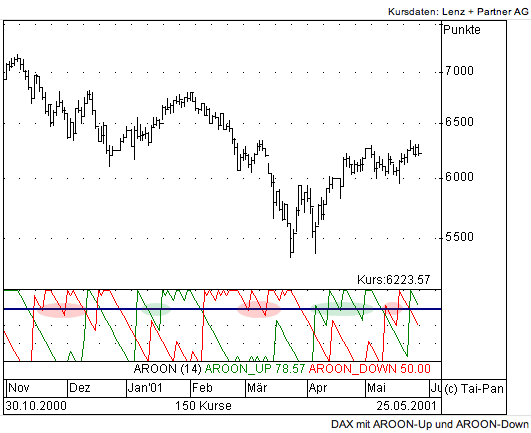
\includegraphics[width=0.8\textwidth]{graphics/chapter2/fingrundlagen/aroon.png}
	\caption[Aroon Indicator]{14-Tage Aroon �ber 7 Monate des DAX-Kurses}
	\label{fig:aroon}
\end{figure}

Die Berechnung des Aroon-Up und Aroon-Down ist mit den folgenden Formeln beschrieben. Wobei $high_{n+1}$ in \ref{Aroon-Up} die Zeit seit dem h�chstem Hoch innerhalb von $n+1$ Perioden und $low_{n+1}$ in \ref{Aroon-Down} die Zeit seit dem tiefstem Tief innerhalb von $n+1$ Perioden bezeichnet.

\begin{equation}
	\label{Aroon-Up}
	\frac{n-high_{n+1}}{n}*100
\end{equation}

\begin{equation}
	\label{Aroon-Down}
	\frac{n-low_{n+1}}{n}*100
\end{equation}

\subsection{Handelsstrategien}

In diesem Punkt sollen verbreitete Handelsstrategien erl�utert werden, um einerseits potentiell zu testende Algorithmen festzustellen und andererseits eine Grundlage f�r Weiterentwicklung und Kombinationsm�glichkeiten aufzuzeigen.

\subsubsection{Preiskreuzung des Gleitenden Durchschnitts}

Eine simples Tradingmodell, dass von einigen Tradern verwendet wird, basiert auf einer einfachen �berkreuzung eines \gls{ma} �ber den Preis. Es wird dabei angenommen, dass wenn der Preis �ber den \gls{ma} steigt, ein Aufw�rtstrend eingesetzt hat, da der Kurs begonnen hat schneller als der l�ngere Durchschnitt zu steigen. Umgekehrt wird angenommen, dass bei einem Abfall des Kurses unter den \gls{ma} ein Abw�rtstrend folg und daher wird ein short-Signal generiert. Eine zus�tzliche Sicherheit ist gegeben, wenn der \gls{ma} selbst in erwartete Kursrichtung dreht.\\
	Dieser simple Algorithmus hat einige Nachteile. Es ist zu jedem Zeitpunkt ein Signal gegeben, was bedeutet dass immer entweder eine long- oder eine short-Position gehalten wird. Au�erdem verliert diese Strategie bei langen \glspl{ma} nach der Trendumkehr wieder viel des Gewinns, da das Gegensignal erst sp�t generiert wird. Kurze \glspl{ma} erzeugen oft Fehlsignale.

\subsubsection{Verwendung Mehrerer Gleitender Durchschnitte}

Eine h�ufig verwendete Variante zur Signalgenerierung mit \glspl{ma} wird \emph{Double Crossover Method} genannt. Dabei kommen 2 unterschiedlich lange \glspl{ma} zum Einsatz, wobei ein Signal erzeugt wird wenn sich beide schneiden. Kreuzt der kurze \gls{ma} den l�ngeren entsteht ein Kaufsignal, auch \emph{Golden Cross} genannt, und vice versa. Diese Variante erzeugt weniger Fehlssignale, als die direkte Verwendung des Preises, hinkt dem Markt daf�r aber auch st�rker hinterher. Die L�nge der Durchschnitte h�ngt wie immer sowohl vom Handelszeitraum und der gew�nschten Signalanzahl, als auch vom Markt ab.\\
\\
Dieses System kann noch um einen weiteren \gls{ma} raffiniert werden. Der Einsatz dreier Durchschnitte, oder \emph{Triple Crossover Method} verfeinert die Art des Signals. Ein vollst�ndiges Kaufsignal entsteht sobald der kurze �ber dem mittleren, und jener wiederum �ber dem langen \gls{ma} notiert. Eine umgekehrte Anordung ist als Verkaufssignal anzusehen.\\
	Beginnt der kurze Trendfolger �ber den mittleren und anschlie�end auch �ber den langen zu steigen, ist dies als vorbereitendes Kaufsignal zu interpretieren. Wenn der mittlere anschlie�end den langen auch noch von unten schneidet ist das Signal vollst�ndig.\\
	Auf diese Art kann beispielsweise bei unklaren Signalen eine Neutralstellung (i.e. keine Aktien im Portfolio) eingenommen werden oder die Market-Exposure (i.e. Anzahl der Aktien) reduziert werden.\\
	Normalerweise werden f�r solche Systeme \glspl{sma} verwendet, wobei aber besonders bei einem Double Crossover System die Anwendung eines \gls{ema} oder sogar 

\subsubsection{Moving Average Convergence/Divergence}


\clearpage
\section{Voruntersuchung}

\subsection{IST-Erhebung}

Es wird bereits ein Gro�teil des Kapitals in Wertpapieren algorithmisch verwaltet. Daher existiert eine Unmenge an Wissen �ber den Aufbau
von B�rsenalgorithmen und die Anwendung von Indikatoren zur Einsch�tzung von zuk�nftigen Kurswerten. Die meisten dieser Algorithmen basieren auf technischer
Analyse und den simplen Algorithmen die diese mit sich bringt.Bekannte Vertreter davon sind zum Beispiel der MACD und der CCI.
Die meisten Algorithmen benutzen au�erdem eine Zusammensetzung aus verschiedenen \glspl{ma}, um die zu Grunde liegenden Handelsentscheidungen zu treffen.
Aufgrund dieses umfangreichen Wissens ist es m�glich weitere M�glichkeiten zu erforschen und noch besser und sinnvoller handelnde maschinelle Helfer zu kreieren.\\
\\
Ein Problem der aktuellen Situation ist allerdings, das schlechte bzw. umst�ndliche Testing dieser Algorithmen, da wenig Software existiert, die
verifizieren kann ob ein Algorithmus in bestimmten Marktphasen bestimmte Leistungen erbringt. Au�erdem ist es momentan ziemlich kompliziert sich einfach
die gesamte Performance eines solchen Handelsalgorithmus anzusehen. Es gibt hierf�r aber sowohl Gratisquellen, als auch kommerzielle Produkte, von denen man
historische Daten zum Backtesting dar Algorithmen beziehen kann. Das Projektteam von Noctua besitzt bereits ca. 3.9 Gb an historischen B�rsenkursen von
e-Signal \footnote{http://www.esignal.com/default.aspx?tc=} und nahezu unbegrenzten Zugriff auf weitere Daten vom selben Anbieter.
Dadurch ist es ihm m�glich Algorithmen �ber ein weites Spektrum von Marktphasen und -zust�nden hinweg zu testen und die Performance verschiedener Algorithmen in unterschiedlichen Situationen akkurat festzustellen. Dies ist besonders wichtig, da Algorithmen die in der nahen Vergangenheit guten Entscheidungen trafen, meist weiterhin sehr erfolgreich handeln und den Anleger m�glicherweise mit einem Kapitalzuwachs belohnen.

\subsection{IST-Zustand}

Aufgrund der riesingen Industrie die diesem Projekt zu Grunde liegt gibt es nat�rlich bereits eine Vielzahl an Konkurrenzprodukten auf dem Markt. Einige davon spezialisieren sich auf das Backtesting bzw. die Bereitstellung einer Plattform zur Entwicklung von Algorithmen. Andere sind eher propriet�rer Natur und versuchen lediglich durch Korruption der Konkurrenz, selbst den wirtschaftlich rentabelsten Algorithmus zu betreiben. Doch alle haben ihre Vor- und Nachteile. Daher finden sich auch immer wieder neue Nieschen f�r Neueinsteiger am Markt, die durch ausgekl�gekte Algorithmen viel erreichen k�nnen. Im folgenden werden nun die bekanntesten dieser Konkurrenzprodukte berschrieben.

\subsubsection{MetaTrader 5}

Hierbei handelt es sich um ein ziemlich umfangreiches, ein wenig �lteres Produkt, dass sowohl Aktien- als auch Forex-Daten anbietet. MetaTrader 5 ist die neue verbesserte Version von Metatrader 4 und bietet neben den alten Funktionen, Neuerungen wie die Einbindung von News. Au�erdem bietet der MetaTrader ein weites Spektrum an Indikatoren, die einfach in den laufenden Betrieb eingebunden werden k�nnen. Die Oberfl�che des MetaTraders sieht in etwa aus, wie in Abbildung \ref{fig:metatrader5_overview} dargestellt.

\begin{figure}
	\centering
		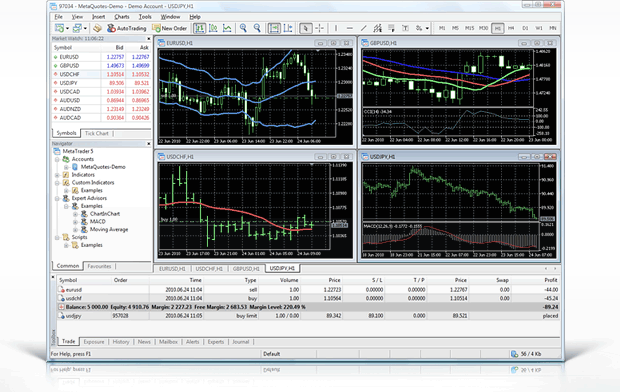
\includegraphics{graphics/chapter2/metatrader5_overview.png}
	\caption{MetaTrader 5 Oberfl�che}
	\label{fig:metatrader5_overview}
\end{figure}

\begin{figure}
	\centering
		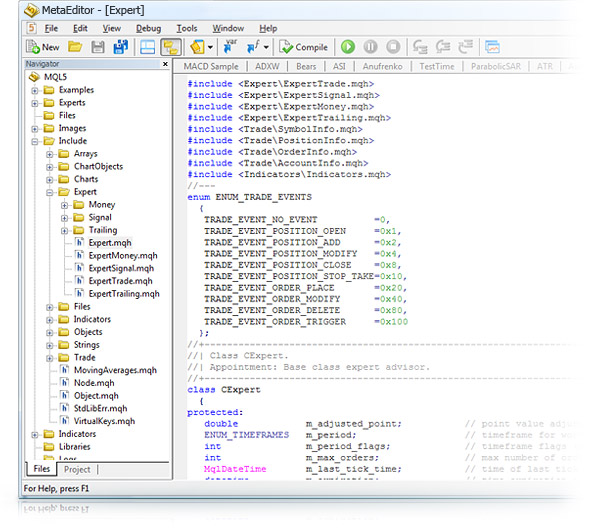
\includegraphics{graphics/chapter2/metaeditor_robot_modification.jpg}
	\caption{MetaTrader 5 IDE-Oberfl�che}
	\label{fig:metaeditor_robot_modification.jpg}
\end{figure}

Doch das gr��te Feature des MetaTraders ist die eingebaute IDE(siehe Abbildung \ref{fig:metaeditor_robot_modification.jpg}), die es mittels einer eigenen MetaTrader-spezifischen Sprache, der \gls{mql5}, erm�glicht eigene Algorithmen zu programmieren und diese dann auch direkt in den laufenden Betrieb zu �bernehmen. Der MetaTrader bietet sogar einen j�hrlichen Wettberewerb an, bei dem er jedes Jahr einen der besten Algorithmen zum Sieger k�rt. Die neue Sprache \gls{mql5} ist sogar ebenfalls noch weiter gegen�ber der MQL4 verbessert. Dies f�hrt uns allerdings auch schon zum Problem beim MetaTrader 5, da nur ein geringer Teil der Software Entwickler gewillt ist, wirklich extra eine neue Programmiersprache zu lernen, nur einen Algorithmus entwicklen und testen zu k�nnen, der dann selbst wiederum auch an den MetaTrader gebunden ist nich in den normalen operativen Betrieb portiert werden kann. Au�erdem ist der MetaTrader eines der sehr wenigen Produkte am Markt, die es Nutzern wirklich erm�glicht einen Algorithmus zu entwickeln und zu testen ohne die gesamte struktur rundherum zuerst aufzubauen. Daher ist es n�tig diesem Mangel Abhilfe zu schaffen und eine \gls{bts} zu entwicklen, die genau dies erm�glicht und ohne den Nutzer dabei an das Unternehmen in dem er seinen Algorithmus testet zu binden.

\clearpage
\chapter{Produktfunktionen} \label{chapter:produktfunktionen}

\section{Must-Have}

/F010/\\
\textit{Vergangene Marktzust�nde bestimmen}

\begin{center}

\begin{tabular}{ | l | p{10cm} |}
\hline 
Beschreibung & Es sollen historische Marktzust�nde (innerhalb der letzten Jahre), auf transparenten
Aktienm�rkten, f�r die ein ausreichender Datenbestand vorhanden ist, automatisch bestimmt
werden. Sollten sich verschiedene gro�e M�rkte entgegen Erwartung entsprechend
unterschiedlich verhalten, dass diese keiner einheitlichen Analyse unterzogen werden k�nnen,
soll prim�r der US-amerikanische Aktienmarkt untersucht werden. Hierbei handelt es sich um
eine Gruppierung von Zeitabschnitten nach gemeinsamen Kriterien.\\  \hline
Aufwand & Hoch \\ \hline
Nutzen & Hoch \\ \hline
Ziel & Ermittelung von Klassen f�r Marktzust�nde. \\ \hline
Vorbedingungen & - \\ \hline
Nachbedingungen & - \\ \hline

\end{tabular}

\end{center}

/F020/\\
\textit{Aktuellen Marktzustand bestimmen}

\begin{center}

\begin{tabular}{ | l | p{10cm} |}
\hline 
Beschreibung & Dabei soll darauf geachtet werden, dass f�r eine fr�he Erkennung m�glicherweise nur ein Teil
der Daten vorhanden ist, die f�r die historische Analyse herangezogen werden.\\  \hline
Aufwand & Mittel \\ \hline
Nutzen & Hoch \\ \hline
Ziel & Zuordnung des aktuellen Marktzustandes zu einem bereits Bekannten. \\ \hline
Vorbedingungen & /F010/ Vergangene Marktzust�nde bestimmen \\ \hline
Nachbedingungen & - \\ \hline

\end{tabular}

\end{center}

/F110/\\
\textit{Trends erkennen}

\begin{center}

\begin{tabular}{ | l | p{10cm} |}
\hline 
Beschreibung & Durch \glspl{ma} soll es m�glich sein Trends in Aktienkursen zu identifizieren. Dazu
kommen verschiedene Crossover-Verfahren (double- / triple-crossover) oder Indikatoren, wie
der MACD (Moving Average Convergence Divergence) in Frage. Es soll eine statistisch
m�glichst profitable Variante hierf�r gefunden werden, die aufscheinende nachhaltige Trends
m�glichst g�nstig erkennt.\\  \hline
Aufwand & Hoch \\ \hline
Nutzen & Hoch \\ \hline
Ziel & Fr�hzeitige m�glichst profitable Erkennung von Trends. \\ \hline
Vorbedingungen & - \\ \hline
Nachbedingungen & - \\ \hline

\end{tabular}

\end{center}

/F120/\\
\textit{\gls{ma}-Dauer bestimmen}

\begin{center}

\begin{tabular}{ | l | p{10cm} |}
\hline 
Beschreibung & Je nachdem, wie lange ein Trend andauert, bedingt eine Trenderkennung andere \gls{ma}(-Paare)
mit unterschiedlichen Laufzeiten. Aus z.B. bew�hrten Wertepaaren oder adaptiven Methoden sollen
automatisch die optimalen Laufzeiten gew�hlt werden.\\  \hline
Aufwand & Niedrig \\ \hline
Nutzen & Mittel \\ \hline
Ziel & Erarbeitung eines optimalen Parametersatzes f�r ein \gls{ma}-Paar. \\ \hline
Vorbedingungen & - \\ \hline
Nachbedingungen & - \\ \hline

\end{tabular}

\end{center}

/F130/\\
\textit{An Marktzustand anpassen}

\begin{center}

\begin{tabular}{ | l | p{10cm} |}
\hline 
Beschreibung & Der Algorithmus soll sich durch Parameterver�nderung an den erkannten Marktzustand zur
Optimierung der Performance anpassen. Dies kann beispielsweise durch ver�ndern der \gls{ma}-Paare
oder durch Anpassung der Market Exposure und damit des Risikos erfolgen.
Dazu \textit{k�nnen} die Implikationen durch Nachforschung bekannt sein, woraufhin ein Modell
angewandt wird, m�ssen aber nicht, da auch induktiv aus den Implikationen gelernt werden
kann, wonach automatisch ein Modell entsteht. (\textit{Maschinelles Lernen}) Dabei werden f�r die
unterschiedlichen Markzust�nde verschiedene Parameters�tze durchprobiert.\\  \hline
Aufwand & Hoch \\ \hline
Nutzen & Hoch \\ \hline
Ziel & Anpassung der Hauptfunktionen des Algorithmus an den aktuellen Marktzustand. \\ \hline
Vorbedingungen & /F020/ Aktuellen Marktzustand bestimmen \\ \hline
Nachbedingungen & - \\ \hline

\end{tabular}

\end{center}

/F140/\\
\textit{Signale generieren}

\begin{center}

\begin{tabular}{ | l | p{10cm} |}
\hline 
Beschreibung & Signalgeben bei potentiellen Einstiegspunkten (long signal) und Ausstiegspunkten (short
signal).\\  \hline
Aufwand & Niedrig \\ \hline
Nutzen & Hoch \\ \hline
Ziel & R�ckgabe von Handelssignalen. \\ \hline
Vorbedingungen & /F110/ Trends erkennen, /F130/ An Marktzustand anpassen, /F120/ \gls{ma}-Dauer bestimmen \\ \hline
Nachbedingungen & /F160/ Signale filtern \\ \hline

\end{tabular}

\end{center}

/F150/\\
\textit{Trend-Nachhaltigkeit bestimmen}

\begin{center}

\begin{tabular}{ | l | p{10cm} |}
\hline 
Beschreibung & Durch geeignete Support- und Resistance-Indikatoren soll die Nachhaltigkeit eines Trends
bestimmt werden (beispielsweise Pivot Points, RSI, CCI oder MAs), um den Ausstiegspunkt zu
optimieren.\\  \hline
Aufwand & Mittel \\ \hline
Nutzen & Hoch \\ \hline
Ziel & Festellen der Nachhaltigkeit erkannter Trends. \\ \hline
Vorbedingungen & /F140 Signale generieren \\ \hline
Nachbedingungen & - \\ \hline

\end{tabular}

\end{center}

/F160/\\
\textit{Signale filtern}

\begin{center}

\begin{tabular}{ | l | p{10cm} |}
\hline 
Beschreibung & Zur Verminderung von unprofitablen, zu kurzen Trades sollen insbesondere Kaufsignale
gefiltert werden. Die Trenderkennung k�nnte des �fteren zu kurz anhaltende Trends
erkennen, indem beispielsweise ein MA-Crossover nur f�r kurze Zeit besteht. Durch das
Einf�hren eines Schwellenwertes (threshold), der �berschritten werden muss, oder eine
bestimmte Zeitspanne, die ein Signal �berdauern muss k�nnen zu kurze Trades vermindert
werden, wenn sich im Backtesting dadurch ein Vorteil herausgestellt hat.\\  \hline
Aufwand & Mittel \\ \hline
Nutzen & Hoch \\ \hline
Ziel & Filterung der unbrauchbaren Signale. \\ \hline
Vorbedingungen & /F140/ Signale generieren, /F150/ Trend-Nachhaltigkeit bestimmen \\ \hline
Nachbedingungen & - \\ \hline

\end{tabular}

\end{center}

/F210/\\
\textit{Performance berechnen}

\begin{center}

\begin{tabular}{ | l | p{10cm} |}
\hline 
Beschreibung & Die relative Performance eines Algorithmus soll in Prozent der Kapitalver�nderung berechnet
werden.\\  \hline
Aufwand & Mittel \\ \hline
Nutzen & Hoch \\ \hline
Ziel & Berechnung der relativen Performance eines Algorithmus \\ \hline
Vorbedingungen & - \\ \hline
Nachbedingungen & - \\ \hline

\end{tabular}

\end{center}

/F220/\\
\textit{Gewinn/Risiko-Verh�ltnis berechnen}

\begin{center}

\begin{tabular}{ | l | p{10cm} |}
\hline 
Beschreibung & Bestimmung des Risikos des Algorithmus (beispielsweise anhand der Volatilit�t) in
Verbindung mit der Performance (e.g. sharpe ratio).\\  \hline
Aufwand & Niedrig \\ \hline
Nutzen & Mittel \\ \hline
Ziel & Bestimmung des Gewinn/Risiko-Verh�ltnisses eines Algorithmus \\ \hline
Vorbedingungen & /F210/ Performance berechnen \\ \hline
Nachbedingungen & - \\ \hline

\end{tabular}

\end{center}
\clearpage
\section{Technische Machbarkeit}\label{section:Technische Machbarkeit}
\subsection{Variantenbildung}
Die \gls{bts} kann man in jeder erdenklichen Programmiersprache schreiben, allerdings ist es wichtig daran zu denken, dass das Programm einerseits effizient arbeiten soll und deswegen hardwarenahe rechnet, und andererseits hat das Projektteam mit manchen Programmiersprachen keinerlei Erfahrung.\\
Die allgemeine Funktionalit�t muss das lesen und schreiben von Dateien sein, aber auch das algorithmische Rechnen soll effizient funktionieren. F�r das Team kommen daher 3 M�glichkeiten in Frage: Eine L�sung in reinem C++, welches sehr hardwarenahe arbeitet, eine Mischung aus F\# und C\#, mit der eine paralelisierte Berechnung m�glich w�re, und eine Java-L�sung, bei der das Team die gr��te Erfahrung mitbringt. \\
Bei der Kombination agiert C\# als Handlungs- und Steuerkern und F\# als funktionale Programmiersprache, als Rechenkern und \"Mastermind\" der Applikation, welches die Entscheidungen trifft. Hierbei wird einerseits eine enorm hohe Arbeitsgeschwindigkeit erm�glicht, da die beiden Sprachen relativ hardwarenah agieren und andererseits besteht der nicht zu untersch�tzende Vorteil bzw. die M�glichkeit, den Rechenkern auf ein externes System outzusourcen, welches zum Beispiel enorme Rechenkapazit�ten aufweisen k�nnte und somit viel komplexere und effizientere Algorithmen in annehmbarer Zeit durchrechnen und abh�ngig davon mehr gewinnbringende Entscheidungen treffen k�nnte. Dabei sollte es auch bei sp�teren Erweiterungen des Programms zu keinem signifikanten Geschwindigkeitsabfall kommen.


\begin{center}

\begin{tabular}{ | c | p{2.6cm} | p{1.7cm} | p{0.5cm} |p{0.5cm}|p{0.5cm}|p{0.5cm}|p{0.7cm}|p{0.7cm}|}
\hline 
\multicolumn{2}{|p{1.5cm}|}{ }  & Gewicht\-ung & \multicolumn{2}{p{1.5cm}|}{\textbf{C++ R*G}} & \multicolumn{2}{p{1.5cm}|}{\textbf{Java R*G}} & \multicolumn{2}{|p{1.5cm}|}{\textbf{C/F R*G}}\\ \hline
\multirow{6}{*}{Einfachheit} & Aufwand Coding & 10\% & 3 & 30 & 1 & 10 & 2 & 20 \\ \cline{2-9}
& Bedinung/ Wartung & 6\% &3&9&2&6&1&3\\ \cline{2-9}
& Update &3\%&3&9&2&6&1&3\\ \cline{2-9}
& Integration &5\%&3&15&2&10&1&5\\  \cline{2-9}
& Kenntnisse &6\%&3&18&1&6&2&12\\ \cline{2-9}
& \textbf{Gesamt}&30\%&3&90&2&44&1&46\\ \hline
\multirow{5}{*}{Leistung}& �bertragungs-zeit &6\%&1&6&3&18&2&12\\ \cline{2-9}
& Absturz-sicherheit &5\%&1&5&2&10&3&15\\ \cline{2-9}
& Ressourcen-verbrauch &3\%&1&3&3&9&2&6\\ \cline{2-9}
& Datenumfang &1\%&1&1&3&3&2&2\\ \cline{2-9}
& \textbf{Gesamt} &15\%&1&15&3&50&2&35\\ \hline
\multirow{5}{*}{Kosten}& Lizenzen &10\%&1&10&1&10&&\\ \cline{2-9}
& Support &5\%&3&15&1&5&2&10\\ \cline{2-9}
& Betriebs-kosten &\%&&&&&&\\ \cline{2-9}
& Dokumen-tation &5\%&1&5&2&20&3&15\\ \cline{2-9}
& \textbf{Gesamt} &\%&&&&&&\\ \hline
\multirow{4}{*}{Dokumentation}& Verf�gbarkeit &10\%&3&30&2&20&1&10\\ \cline{2-9}
& Voll-st�ndigkeit &10\%&3&30&2&20&1&10\\ \cline{2-9}
& Qualit�t &10\%&2&20&1&10&1&10\\ \cline{2-9}
& \textbf{Gesamt} &30\%&3&80&2&50&1&30\\ \hline
\end{tabular}

\end{center} 

\begin{center}

\begin{tabular}{|l|r|p{0.8cm}|p{0.8cm}|p{0.8cm}|p{0.8cm}|p{0.8cm}|p{0.8cm}|} \hline
Kapitel&Gewichtung&\multicolumn{2}{p{1.8cm}|}{\textbf{C++}}&\multicolumn{2}{p{1.8cm}|}{\textbf{Java}}&\multicolumn{2}{p{1.8cm}|}{\textbf{C\#/F\#}}\\ \hline
Einfachheit&30\%&3&90&2&44&1&46 \\ \hline
Leistung&\%&&&&&& \\ \hline
Kosten&\%&&&&&& \\ \hline
Dokumentation&\%&&&&&& \\ \hline
\end{tabular}

\end{center}

\begin{center}
\begin{tabular}{|l|l|l|l|} \hline
Gesamtbewertung&&&\\ \hline
Endreihung &&&\\ \hline
\end{tabular}
\end{center}


\clearpage
% Wirtschaftliche Machbarkeit

\section{Wirtschaftliche Machbarkeit} \label{chapter:Wirtschaftliche Machbarkeit}

\subsection{Aufwandsabsch�tzung}

\subsection{Nutzen}

\subsection{Pr�fen der Risiken}
\subsubsection{Personenausfall}
Eintrittswahrscheinlichkeit:  gering \\
Auswirkungen:  								hoch   \\

In dem unerwarteten Fall, dass ein Teammitglied l�ngerfristig ausf�llt, muss es m�glich sein die Arbeitsaufgaben dementsprechend neu aufteilen zu k�nnen.
Folgende F�lle k�nnten auftreten:
\begin{itemize}
	\item Streit im Team
	\item Ausfall durch Krankheit oder Tod eines Teammitglieds
	\item Austritt eines Teammitglieds aus dem Projekt
	\item Der Auftraggeber k�nnte aufgrund von Unklarheiten den Projektabbruch initiieren 
	\item Es kann passieren, dass von Seite des Auftragsgebers pl�tzlich kein Interesse an der Umsetzung des Produktes mehr gegeben ist, und es dadurch zu extremem Zeitverzug kommt, was bis zum Abbruch f�hren kann
	\item Interessensverlusst eines Teammitglieds, und damit verbundene minderwertigere Arbeit 
\end{itemize}

Folgende pr�ventive Ma�nahmen werden eingef�hrt:
\begin{itemize}
	\item Regeln f�r den Umgang innerhalb des Projekts
	\item Ausreichendes Interesse jedes Mitglieds und keine leistungstechnische Probleme 
	\item Gutes Verh�ltnis mit den Auftraggebern
\end{itemize}

\subsubsection{Zeitliche Risiken}

Eintrittswahrscheinlichkeit:  gering \\
Auswirkungen:  								mittel \\

Die Aufwands- und Zeitsch�tzung basiert auf dem derzeitigen Lastenheft des Auftraggebers und stellt eine zeitgerechte Fertigstellung sicher. Sollten sich jedoch die Anforderungen des Kunden w�hrend des Projekts �ndern, so wird sich das mit gro�er Wahrscheinlichkeit verz�gernd auf den Fertigstellungstermin auswirken. Die mit dem Kunden vereinbarte Funktionsanalyse und die Meilensteine mit gemeinsam festgelegten Qualit�tskriterien sollten jedoch diesem Risiko entgegenwirken.

\subsubsection{Technische Risiken}
\label{subsection:Technische Risiken}
\textbf{Datenverlust}\\
Eintrittswahrscheinlichkeit:  gering \\
Auswirkungen:  								mittel \\

Aufgrund der nicht auszuschlie�enden Gefahr des Datenverlusts, muss daf�r gesorgt werden die Sicherheit der Daten, sowie auch die Verf�gbarkeit dieser zu garantieren. Dieses Problem wird mithilfe eines \gls{git} gel�st, durch diesen Server ist es m�glich die Versionen der Software immer zug�nglich zu machen und zus�tzlich die Daten auf den Computern der Projektmitgliedern zu speichern. \\ \\

\textbf{Hardwareausfall} \\
Eintrittswahrscheinlichkeit: gering \\
Auswirkung: mittel \\

Es kann ohne jede Vorwarnung immer und �berall ein Hardwareausfall passieren, dies kann selbst verschuldet, aber auch pl�tzlich passieren. Um mit einem solchen Ausfall zurecht zu kommen besitzt das Projektteam einen Ersatzlaptop um das gezielte Arbeiten auch nach dem 
Ausfall garantieren zu k�nnen. \\ \\

\textbf{Versionsverlust} \\
Eintrittswahrscheinlichkeit: sehr gering \\
Auswirkung: mittel \\

Bei den Versuchen mit dem Algorithmus wird andauernd etwas in der Datei ver�ndert. Bei dieser T�tigkeit kann es passieren das die Zusammenh�nge zwischen 1 oder mehreren Versionen des Algorithmus verloren gehen. Bei so einem Verlust kann auch das grundliegende Verst�ndnis f�r die jeweilige Version verloren gehen.\\
Folgende pr�ventive Ma�nahmen werden eingef�hrt:
\begin{itemize}
	\item Verwendung eines \gls{git}, f�r die automatische Versionierung
	\item Zwingende Benutzung der Bugtrackingsoftware
	\item Kommunikation im Team �ber die �nderungen am Algorithmus
\end{itemize}
\clearpage
\chapter{Projektorganisation} \label{chapter:Projektorganisation}

Der Grund daf�r, dass dieses Projekt ins Leben gerufen wurde, ist der Projektauftraggeber Herr Professor Mag. Hans Brabenetz und Herr Professor Dr. Helmut Vana. Der Projektleiter ist Peer Nagy und das Team besteht noch zus�tzlich aus zwei weiteren Entwicklern. Die anderen Projektteammitglieder sind Herr Gabriel Pawlowsky und Herr Josef Sochovsky.
\clearpage
% !TeX root = ../../Noctua_Diplomarbeit.tex

\section{Management Summary}
\label{section:management_summary}

Die Machbarkeitsstudie des Projektes NOCTUA behandelte die kritischen Punkte der Algorithmuskonzeption und -entwicklung und der \gls{bts}.\\
	Ein wichtiger Bestandteil waren Nachforschungen im Bereich der finanzwirtschaftlichen Grundlagen und der Technischen Analyse. Dabei wurden einige Trendfolgemechanismen und Oszillatoren beschrieben, um aus diesen und �hnlichen Mechanismen im Laufe des Projektes einen eigenen Algorithmus entwickeln zu k�nnen.\\
	Da es wichtig ist einen Algorithmus auch w�hrend der Laufzeit der \gls{bts} wechseln zu k�nnen, wird dieser in der Programmiersprache F\# entwickelt und als \gls{dll} gespeichert. Diese \gls{dll} kann einfach �ber eine \gls{gui} ausgew�hlt und f�r die aktuelle Berechnung herangezogen werden.\\
	Laut Aufwandssch�tzung entsteht ein Aufwand von insgesamt 480 h und Kosten in der H�he von \EUR{36.141}.
	
	\section{Versionierung} \label{section:versionierung}
\begin{center}

\begin{tabular}{ | l | p{2cm} | p{2cm} | p{2cm} | p{1.5cm} | p{2.8cm} | }
\hline 
\textbf{Version}�& \textbf{Autor} & \textbf{QS} & \textbf{Datum} & \textbf{Status} & \textbf{Kommentar} \\  \hline
0.1 & Sochovsky & Pawlowsky & 22.09.2012 & draft & Erstversion \\ \hline
0.2 & Pawlowsky & Nagy & 22.09.2012 & draft & Produkt\-funktionen\\ \hline
0.3 & Sochovsky & Pawlowsky & 23.09.2012 & draft & Technische Machbarkeit \\ \hline
0.4 & Sochovsky & Nagy & 24.09.2012 & draft & Nutzwert\-analyse\\ \hline
0.5 & Sochovsky & Pawlowsky & 26.09.2012 & draft & Wirtschaftliche Machbarkeit \\ \hline
0.6 & Nagy & Pawlowsky & 27.09.2012 & draft & Finanz\-wirtschaft\-liche Grundlagen \\ \hline
0.7 & Pawlowsky & Sochovsky & 28.09.2012 & draft & FPA \\ \hline
0.8 & Sochovsky & Nagy & 30.09.2012 & draft & Sollzustand \\ \hline
0.9 & Sochovsky & Nagy & 06.10.2012 & draft & Projekt\-organisation \\ \hline
1.0 & Pawlowsky & Sochovsky & 07.10.2012 & draft & Aufwands\-absch�tzung \\ \hline
1.1 & Nagy & Sochovsky & 15.10.2012 & draft & Einleitung \\ \hline
1.2 & Nagy & Pawlowsky & 17.10.2012 & Entwurf & Management Summary, Nutzen \\ \hline
\end{tabular}

\end{center}

%
% Chapter3

\chapter{Grundlagen} \label{chapter:grundlagen}

%\begin{quotation}
%``The market is not an invention of capitalism. It has existed for centuries. It is an invention of civilization.``
%\begin{flushright}
%(Mikhail Gorbachev)
%\end{flushright}
%\end{quotation}

Aufgabe dieses Kapitels ist es zun�chst ein Fundament f�r das Verst�ndnis dieser Arbeit zu legen und Funktionsweisen, Vorg�nge sowie verschiedene Ans�tze zu erl�utern.\\

\section{Finanzwirtschaftliche Grundlagen}

% !TEX root = ../../Noctua_Diplomarbeit.tex

\subsection{Boerse und Preisbildung}

Eine B�rse ist ein Handelsmarkt, auf dem sich Preise durch Angebot und Nachfrage von Handelspartnern bilden und der Handel nicht direkt zwischen K�ufern und Verk�ufern, sondern �ber berechtigte H�ndler abgewickelt wird. Wichtig ist dabei, dass immer f�r ausreichend Liquidit�t gesorgt werden muss, so dass jederzeit Wertpapiere gekauft und auch verkauft werden k�nnen.

Handelsvorg�nge oder Trades resultieren aus einer Erwartungshaltung der Marktteilnehmer.  \cite{boerse-wien-funktion} \cite{boerse-frankfurt-funktion}
Unter der Annahme von steigenden Kursen werden Einheiten gekauft, i.e. es wird "`long gegangen"', werden fallende Kurse erwartet, werden entweder existierende St�ckzahlen verkauft oder es wird sogar ein Leerverkauf get�tigt, i.e. eine Short-Position er�ffnet. Damit wird der Verkauf von geborgten Wertpapieren bezeichnet, die zu einem sp�teren Zeitpunkt beim Schlie�en der Short-Position erst gekauft werden. Sinken die Kurse dazwischen, wird daher zu einem h�heren Preis verkauft als sp�ter gekauft wird und es entsteht die Differenz als Gewinn. \cite{gabler-leerverkauf}

Wollen mehr Handelsteilnehmer oder \emph{Trader} kaufen als verkaufen, steigt der Preis aufgrund der hohen Nachfrage, man spricht auch von einem Bullenmarkt. \cite{duden-bullenmarkt}
Ist es andersherum so, dass die Verk�ufer �berwiegen und der Preis sinkt, handelt es sich um einen B�renmarkt. \cite{duden-baerenmarkt}\\

F�r jedes Wertpapier wird ein sogenanntes Orderbuch gef�hrt, das die aktuellen Kauf- und Verkaufsauftr�ge beinhaltet. Investoren interessieren sich meist f�r die sogenannte Quote-Zeile, die Informationen zu den g�nstigsten Konditionen sowohl auf K�ufer- als auch auf Verk�uferseite bietet.\\

Eine Quote-Zeile von Apple (AAPL) k�nnte dabei folgenderma�en aussehen.

\begin{center}
\begin{tabular}{|c|c|c|c|}
\hline 
Bid & Bid Size & Ask & Ask Size \\ \hline
691.52 & 7 & 691.66 & 3 \\ \hline
\end{tabular}
\end{center}

Der Bid-Preis von \textdollar{691.52} ist das h�chste vorhandene Gebot f�r eine Apple-Aktie. Die Bid-Size gibt die Information �ber die Anzahl an Aktien, die K�ufer zu diesem Preis erstehen wollen. Die Anzahl wird in \emph{round lots} angegeben; meist entspricht ein Round Lot 100 St�ck der Aktie. Die Bid-Seite beschreit somit die K�uferseite. Der Ask-Preis und die Ask-Size beschreibt hingegen das beste Angebot auf der Verk�uferseite. In diesem Fall werden 3 Round Lots f�r den St�ckpreis von \textdollar{691,66} pro Aktie angeboten. Ein Round Lot w�rde in diesem Fall also \textdollar{69166,00} kosten.

Soll ein Handel schnellstm�glich abgewickelt werden muss zum Ask-Preis gekauft und zum Bid-Preis verkauft werden. Wird in diesem Fall mindestens die Ask- bzw. Bid-Size gehandelt, ver�ndert sich die Quote-Zeile so, dass das n�chstbeste Angebot angezeigt wird. Diese Hintereinanderreihung von Angeboten wird auch als Orderbuchtiefe bezeichnet. \\
Angenommen, ein K�ufer ist nicht bereit zum aktuellen Ask-Preis zu kaufen. Er will bessere Konditionen und schickt eine \emph{Limit-Order}, d.h. zu gegebenem Preis oder besser \footnote{IB-Ordertypen siehe: http://www.interactivebrokers.com/de/p.php?f=orderTypes}, mit einem Limit, das zwischen Ask- und Bid-Preis liegt. Sein Kaufgebot ist damit h�her als der zuvor h�chste und wird daher sofort in der Quote-Zeile auf der Bid-Seite angezeigt.

Der Aktienkurs wird mithilfe dieser vorhandenen Orders so gebildet, dass stets der h�chste Umsatz entsteht. Bei hoher Nachfrage auf K�uferseite steigt dadurch der Preis, dominieren jedoch die Verk�ufer sinkt dieser. \cite{charttec-kursfeststellung}
% !TEX root = ../../Noctua_Diplomarbeit.tex

\subsection{Markt und Marktzust�nde}

Aktienpreise setzen sich vollst�ndig aus Angebot und Nachfrage zusammen. Nachfrage entsteht, wenn Handelsteilnehmer annehmen, dass die Preise steigen, Angebot durch die Erwartung von negativen Kursverl�ufen.
Diese Annahmen beruhen auf einer Vielzahl von Informationen, die zur Verf�gung stehen. Somit haben diese Informationen einen direkten Einfluss auf die Aktienkurse. Ver�ffentlicht ein Unternehmen seine Bilanz und fallen darin die Gewinne h�her aus als erwartet, wird der Aktienkurs aufgrund dieser Information steigen. Die Preise reflektieren aber nicht nur realisierte Gewinne, sondern auch potentiell zuk�nftige. W�ren in der Theorie alle m�glichen Informationen allen Handelsteilnehmern bekannt, w�rde sich der Kurs nur mehr durch das Auftauchen von neuen Informationen ver�ndern. In der Praxis verh�lt es sich anders, da weder alle Informationen vorhanden sind, noch Handelsteilnehmer absolut rational agieren.

Diese in den 1960er-Jahren entwickelte Theorie wird als \emph{Efficient Market Hypothesis} bezeichnet und besagt kurz gefasst, dass Marktpreise alle verf�gbaren Informationen vollst�ndig widerspiegeln.\\
Au�er der Schlussfolgerung, dass Nachrichten und Ereignisse f�r Preisentwicklungen h�chst relevant sind, l�sst sich ebenfalls folgern, dass positive Informationen, z.B. eine Wachstumsprognose, keinen Kursanstieg bedeuten m�ssen, weil diese Informationen schon im aktuellen Marktpreis enthalten sein k�nnen. \cite{lo-efficient-market-hypothesis}\\
Unter der Pr�misse, dass die Efficient Market Hypothesis uneingeschr�nkte G�ltigkeit besitzt, l�sst sich au�erdem deduzieren, dass zuk�nftige Preise nicht vorhersehbar sind. W�re dies n�mlich der Fall und k�nnte jeder Markteilnehmer die Preise beliebig genau vorhersagen, w�re niemand bereit, unter dem vorhergesagten Preis zu verkaufen und niemand w�rde dar�ber kaufen. Daraus resultiert, dass der Aktienmarkt den vorhergesagten Preis fixiert. Da nur neue Informationen, die noch nicht bekannt sind, das Preisniveau ver�ndern, sind folglich auch die Preise noch nicht bekannt. \cite{bodie-investments}\\

Da ein Marktpreis bei erh�hter Nachfrage steigt, ist es f�r Aktienanleger sinnvoll, Geld dort anzulegen, wo auch andere investieren. Ein Vorteil liegt daher darin, herauszufinden, was die Mehrheit oder der Markt denkt und nicht in der pers�nlichen Einsch�tzung des Wertes. John Maynard Keynes beschreibt diese Theorie schon 1936 in seiner \emph{General Theory}.\\
In dieser Theorie l�sst sich eine R�ckkopplung zur Information erahnen. Nicht nur die urspr�ngliche Information selbst spielt eine Rolle, sondern auch die Reaktion darauf, im Falle von Aktien also die Kursentwicklung. Dieser iterative Prozess ben�tigt aufgrund von menschlichem Handeln aber auch seine Zeit. Deshalb entstehen durch Kursschwankungen und die verursachten Reaktionen Trendbewegungen in den M�rkten. Erst durch diesen eigentlich psychologischen Effekt funktionieren Charttechniken und technische Analysen.\\
F�r jene, die sich zus�tzlich noch mit makro�konomischen Zusammenh�ngen befassen, besteht trotzdem weiterhin ein Vorteil. Marktr�ckkopplungen unterliegen einem "`Herdentrieb"' und k�nnen zu Spekulationsblasen f�hren. �bergeordnete Vorg�nge k�nnen somit fr�hzeitige Hinweise liefern und bei der korrekten Interpretation der resultierenden Kursverl�ufe helfen. \cite{singer-herdentrieb}

Um die Performance von Trendfolgemethoden zu optimieren, sollen verschiedene Marktzust�nde unterschieden werden, die sich auf den Kursverlauf auswirken. Zu diesem Zweck k�nnen diverse Kriterien untersucht werden, angefangen bei unterschiedlich langen Trendverl�ufen, pl�tzliche Kursbewegungen, Dauer eines Trends usw.\\
Beispielsweise k�nnte sich herausstellen, dass bei einem sehr langfristigen Aufw�rtstrend bei Kaufsignalen die Long-Positionen immer gr��er ausfallen sollten als die Short-Positionen bei Verkaufssignalen oder dass erh�hte Volatilit�t einen Kurseinbruch oder eine Trendumkehr ank�ndigen.\\

\begin{figure}
	\centering
		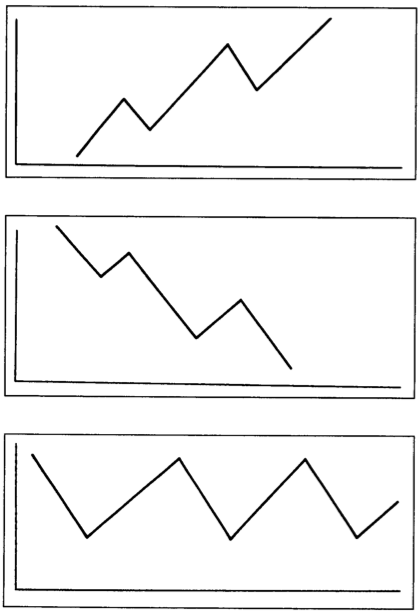
\includegraphics[width=0.8\textwidth]{graphics/fingrundlagen/trend_types.png}
	\caption[Typen von Trends]{Typen von Trends: Aufw�rts-, abw�rts und seitw�rts gerichteter Markt \cite{murphy-technische}}
	\label{fig:trend_types}
\end{figure}

Bei der Trendbestimmung in B�rsenkursen gelten gleitende Durchschnitte, oder \glspl{ma}, als ein beliebtes Mittel und infolge dessen h�ufig genutzter Indikator. Die klassische technische Analyse ist oft subjektiv und unterliegt einem gewissen Interpretationsspielraum, w�hrend algorithmische Handelssysteme klare Entscheidungen generieren m�ssen, weshalb einerseits immer wieder Fehlentscheidungen getroffen werden, andererseits das Handelssystem ausreichend viele Faktoren einbeziehen sollte.

Ein \gls{ma} ist, wie der Name bereits verr�t, eine Art statistischer Durchschnitt einer Reihe von Werten. "`Gleitend"' oder "`moving"' bedeutet, dass nicht alle historischen Daten in die Durchschnittsberechnung einflie�en, sondern nur eine beschr�nkte Anzahl der vergangenen Daten. Es gibt unterschiedliche Varianten von \glspl{ma}, die sich darin unterscheiden wie viele historische Daten verwendet werden und wie die einzelnen Datens�tze gewichtet werden. Klassisch werden Schlusskurse zur \gls{ma}-Berechnung verwendet, wobei manche Trader es vorziehen, Open- oder Mittelwerte aus Open- und Close heranzuziehen. Eine weitere Variante ist eine sepa\-rate Berechnung von \glspl{ma} f�r High- und Low-Kurse, wodurch ein Band entsteht, das eine Art Neutralbereich anzeigt, der beispielsweise als Signalfilter verwendet werden kann. Prinzipiell sind alle \glspl{ma} Trendfolge-Indikatoren, sie antizipieren keine zuk�nftigen Kursver�nderungen, wie viele andere Methoden der technischen Analyse, sondern reagieren nur auf bereits stattgefundene Trendwenden.\\
% !TEX root = ../../Noctua_Diplomarbeit.tex

\subsection{Unterst�tzung und Widerstand}

Die Kurse von Aktien unterliegen, wie bereits erw�hnt, gewissen Trends, die entweder auf-, ab- oder auch seitw�rts (weder auf- noch abw�rts) verlaufen. Bei steigenden Kursen erreichen diese irgendwann ein Level, bei dem der Preis nicht mehr als billig angesehen wird und der Kurs dreht sich um. Der Trend verliert also seine Nachhaltigkeit. Dieses Level wird als \emph{Widerstand} oder \emph{Resistance} bezeichnet, da es nur schwer �berwunden wird. Sinkt der Kurs eine Weile wieder und sonstige Bewertungskriterien des Handelsgutes haben sich nicht signifikant ver�ndert, erreicht der Kurs einen Punkt, bei dem er wieder interessant f�r etwaige K�ufer wird. Diese Schwelle wird als \emph{Unterst�tzung} oder \emph{Support} bezeichnet. \cite{elder_living} Am Beispiel von Microsoft kann diese Funktion in der Abbildung \ref{fig:msft_sup_res} �ber einen l�ngeren Zeitraum beobachtet werden\\

Diese beiden Schwellen sind tempor�re Hilfsmittel und lassen Wendepunkte erahnen. Beim Durchbruch eines Levels kann hingegen mit einer Fortsetzung dieses Trends gerechnet werden und ggf. wird ein alter Widerstand zur Unterst�tzung. \cite{investopedia-support-resistance} Abbildung \ref{fig:payx_sup_res} von Paychex Inc. veranschaulicht diesen Wechsel von Unterst�tzungs- zu Widerstands- und wieder zur�ck zu Unterst�tzungsleveln.

\begin{figure}
	\centering
		\includegraphics[width=0.8\textwidth]{graphics/fingrundlagen/msft_sup_res.JPG}
	\caption[Microsoft Support Resistance]{Microsoft 5-Jahres-Chart mit 1-Wochen-Intervallen und eingezeichneten Support- und Resistance-Leveln}
	\label{fig:msft_sup_res}
\end{figure}

\begin{figure}
	\centering
		\includegraphics[width=0.8\textwidth]{graphics/fingrundlagen/payx_sup_res.JPG}
	\caption[Paychex Inc. Support Resistance]{Paychex Inc. 5-Jahres-Chart mit 1-Wochen-Intervallen; Level wechselt zwischen Support- und Resistance-Funktion}
	\label{fig:payx_sup_res}
\end{figure}
% !TEX root = ../../Noctua_Diplomarbeit.tex

\subsection{Indikatoren} \label{Indikatoren}

%%%%%%%%%%%%%%%%%%%%%%%%%%%%%%%%%%%%%%%
\subsubsection{Simple Moving Average}

Die einfachste M�glichkeit, um Trends in Aktienkursen sichtbar zu machen, ist eine Gl�ttung des Preisverlaufs, also eine Art Durchschnittsberechnung.
Dadurch erh�lt man einen stabileren �berblick �ber die Richtung, in die sich der Kurs bewegt, ohne dass einmaligen Ausbr�chen zu viel Gewicht geschenkt wird.

Bei einem \gls{sma} wird f�r jeden neuen Wert jeweils aus den letzten $n$ Werten ein arithmetischer Mittelwert berechnet. Soll aus einer Reihe von Close-Kursen ein 10-Tages-\gls{sma} berechnet werden, werden dazu die letzten 10 Schlusskurse addiert und anschlie�end durch 10 dividiert, um einen Wert zu erhalten. F�r den folgenden Mittelwert wird der �lteste subtrahiert, ein weiterer neuer Wert addiert und die Summe anschlie�end wieder f�r einen Mittelwert durch 10 dividiert. Auf diese Weise entsteht ein gegl�tteter Kurs, der kurzzeitige Preisver�nderungen abschw�cht, wodurch Trends klarer erkennbar werden.

Zwei h�ufig kritisierte Eigenschaften des \gls{sma} sind, dass erstens nicht alle vorhandenen Daten in die Berechnung einbezogen werden und zweitens alle verwendeten Kursdaten mit gleicher Gewichtung in das Resultat eingehen. Bei einem 10-Tage-\gls{sma} hat jeder Kurswert, unabh�ngig vom Alter, eine Gewichtung von 10\%, bei einem 20-Tage-\gls{sma} 5\%.\\

Ein \gls{sma} wird wie folgt berechnet:

\begin{equation}
	\label{Simple Moving Average}
	P^{*}_t = \frac{1}{n} * \sum\limits_{i=0}^n{P_{t-i}}
\end{equation}

Dabei ist $P^{*}_t$ der gegl�ttete Wert zum Zeitpunkt $t$, $n$ die Anzahl an einbezogenen Werten und $P_{t-i}$ der Preis zum Zeitpunkt $t-i$. \cite{elder_living} \cite{murphy-technische}

\begin{figure}
	\centering
		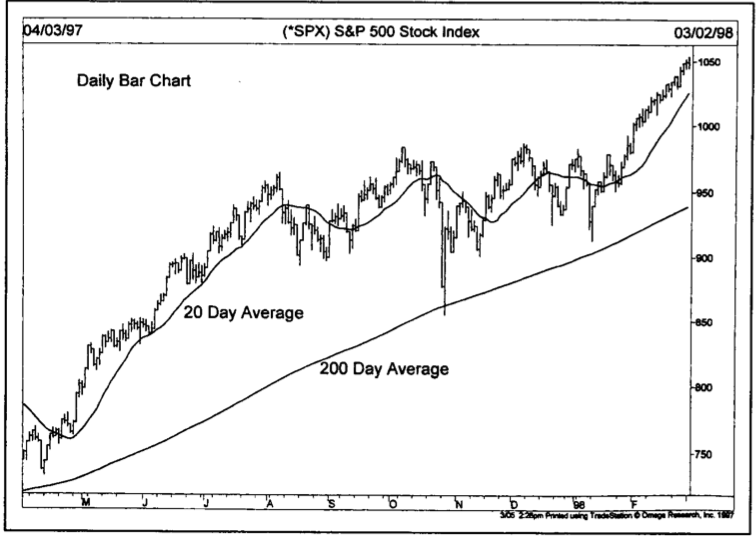
\includegraphics[width=0.8\textwidth]{graphics/fingrundlagen/sma.png}
	\caption[20- und 2-Tage SMA]{Vergleich eines 20- und 2-Tage SMA \cite{murphy-technische}}
	\label{fig:sma}
\end{figure}

%%%%%%%%%%%%%%%%%%%%%%%%%%%%%%%%%%%%%%%
\subsubsection{Linear Weighted Moving Average}

Um eines der Probleme des \gls{sma} zu vermeiden, n�mlich die gleiche Gewichtung aller Daten �ber die Zeit, kann ein \gls{lwma} verwendet werden. Dabei werden Daten zu fr�heren Zeitpunkten geringer gewichtet, als aktuellere Daten. Konkret wird der neueste Eintrag mit $n$ multipliziert, der vorangehende mit $n-1$ und so weiter bis der letzte den Multiplikationsfaktor 1 erh�lt. Die daraus gebildete Summe muss anschlie�end noch durch die Summe der Multiplikatoren dividiert werden, um einen Durchschnitt zu erhalten. Bei einem 10-Tage-\gls{lwma} werden die Kursdaten von neu nach alt mit $10, 9, 8, 7,\dots, 1$ multipliziert und die anschlie�end gebildete Summe durch $10+9+8+7+\dots+1$ dividiert.

\begin{equation}
	\label{Linear Weighted Moving Average}
	P^{*}_t = \frac{\sum\limits_{i=0}^{n-1}{P_{t-i} * (n-i)}}{\sum\limits_{i=0}^{n-1}{i}}
\end{equation}

$P^{*}_t$ ist hier wiederum der gegl�ttete Preis zum Zeitpunkt $t$, $P_t$ der Preis zum Zeitpunkt $t$. \cite{murphy-technische}

%%%%%%%%%%%%%%%%%%%%%%%%%%%%%%%%%%%%%%%
\subsubsection{Exponential Moving Average}

Der \gls{ema} versucht beide Hauptkritikpunkte am \gls{sma} zu l�sen, indem er neuere Werte immer st�rker gewichtet und alle zur Verf�gung stehenden Daten in die Berechnung einbezieht. Man spricht auch vom exponentiell gegl�tteten gleitenden Durchschnitt. Dazu muss ein \emph{\gls{sf}}, auch Gl�ttungsfaktor genannt und meist als $\alpha$ bezeichnet, zwischen 0 und 1 gew�hlt werden, mit dem ein neuer Wert multipliziert wird. Der vorherige Wert wird mit der Differenz des \gls{sf} zu 1 multipliziert. Der aktuelle Wert des \gls{ema} ergibt sich dann aus der Addition dieser beiden gewichteten Werte. Dadurch bleibt jeder Kurswert unendlich lange in der weiteren Berechnung bestehen, die Bedeutung �lterer Kurswerte konvergiert jedoch gegen 0. Aus ebendiesem Grund handelt es sich, mathematisch rigoros betrachtet, beim \gls{ema} nicht wirklich um einen \emph{moving} average, da sich der Wertebereich nicht verschiebt, sondern immer alle Werte zur Berechnung verwendet werden. \cite{klinker-exponential}

Um exponentielle Durchschnittswerte mit normalen \gls{ma}-Werten vergleichen zu k�nnen, wird $\alpha$ meist mit einer Formel berechnet, die n�herungsweise die gleiche Periode f�r ein bestimmtes $n$ ergibt.

\begin{equation}
	\label{Gl�ttungsfaktor alpha}
	\alpha = 2/(n+1)
\end{equation}
	
Soll nur der aktuelle Wert berechnet werden, ist eine rekursive Berechnung naheliegend. Eine m�glichst performante Berechnung einer exponentiell gegl�tteten Zeitreihe beginnt meistens mit einem arithmetischen Mittel �ber die ersten $n$ Werte, um einen Anfangswert zu erhalten, der einen \gls{ema}-Wert besser approximiert, als wenn der erste Preis als Anfangswert herangezogen w�rde.

Die folgende Formel soll die Berechnung des exponentiell gegl�tteten Preises $P^{*}_t$ zum Zeitpunkt $t$ verdeutlichen. Dabei ist $\alpha$ der \gls{sf} und $P^{*}_{t-1}$ der exponentiell gegl�ttete Preis zum Zeitpunkt $t-1$.

\begin{equation}
	\label{Exponential Moving Average}
	P^{*}_t = \alpha * P_{t} + (1 - \alpha) * P^{*}_{t-1}
\end{equation}
\cite{murphy-technische} \cite{elder_living}

\begin{figure}
	\centering
		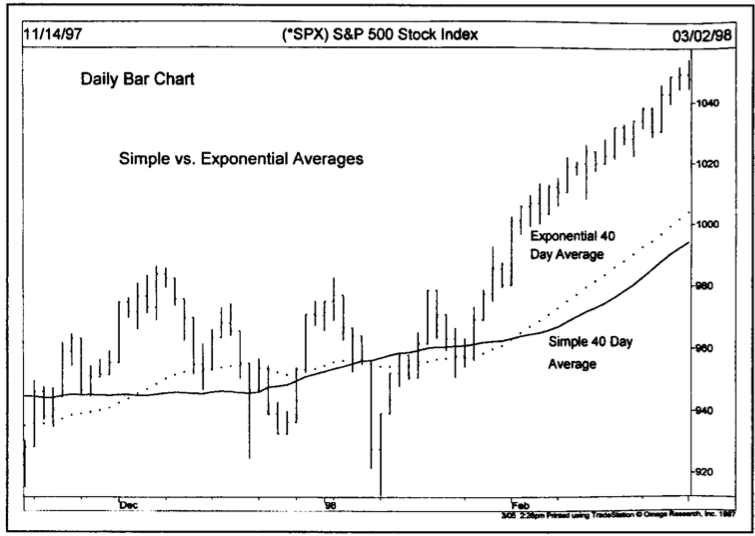
\includegraphics[width=0.8\textwidth]{graphics/fingrundlagen/sma_ema}
	\caption[Vergleich SMA mit EMA]{Vergleich eines 40-Tage SMA mit einem 40-Tage EMA \cite{murphy-technische}}
	\label{fig:sma_ema}
\end{figure}

%%%%%%%%%%%%%%%%%%%%%%%%%%%%%%%%%%%%%%%
\subsubsection{Double und Triple Exponential Moving Average}

Um den Lag, also das Hinterherhinken der gegl�tteten Zeitreihe hinter dem tats�chlichen Kurs, zu reduzieren, gibt es die M�glichkeit, neue Daten noch st�rker zu gewichten als bei einem normalen \gls{ema}.
1994 von Patrick Mulloy eingef�hrt, schaffen sowohl der \gls{dema} als auch der noch st�rker neue Daten gewichtende \gls{tema} bei dieser Problematik Abhilfe.
Den \gls{dema} darf man sich allerdings nicht als \gls{ema} eines bereits berechneten \gls{ema} vorstellen. Das w�rde zu einer unerw�nschten starken Abwertung aktueller Daten f�hren, wie an den Gewichtungsgraphen in Abbildung \ref{fig:wrong_dema_tema} zu sehen ist. Tats�chlich wird der \gls{dema} aus einer Zusammensetzung aus einem einfachen und einem doppelten \gls{ema} berechnet, wodurch ein neuer \gls{ma} mit weniger Lag als jede der Komponenten entsteht. \cite{mulloy-smoothing}

\begin{equation}
	\label{Double Exponential Moving Average}
	DEMA = 2*EMA - EMA(EMA)
\end{equation}

\begin{equation}
	\label{Triple Exponential Moving Average}
	TEMA = 3*EMA - 3*EMA(EMA) + EMA(EMA(EMA))
\end{equation}

\begin{figure}[htbp]
	\centering
	\begin{minipage}[b]{0.4\textwidth}
		\centering
 			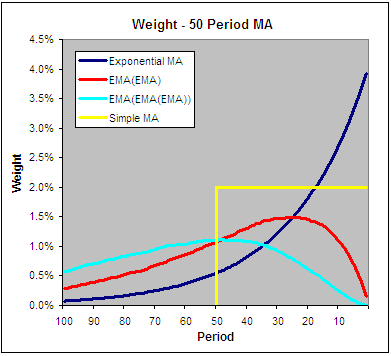
\includegraphics[width=0.9\textwidth]{graphics/chapter2/fingrundlagen/wrong_dema_tema.png}
			\caption[Falsche Multiple Exponential Average Gewichtung]{Falsche Double und Triple Exponential Average Gewichtung}
			\label{fig:wrong_dema_tema}
	\end{minipage}\hspace{0.01\textwidth}	% Abstand zwischen den Bildern = 1% der Textbreite
	\begin{minipage}[b]{0.4\textwidth}
		\centering
 			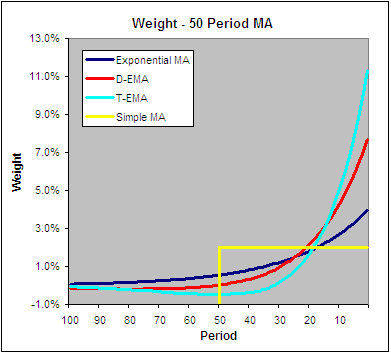
\includegraphics[width=0.9\textwidth]{graphics/chapter2/fingrundlagen/right_dema_tema.png}
			\caption[Richtige Multiple Exponential Average Gewichtung]{Richtige Double und Triple Exponential Average Gewichtung}
			\label{fig:right_dema_tema}
	\end{minipage}
\end{figure}

\cite{etf-hq-dema-tema}

%%%%%%%%%%%%%%%%%%%%%%%%%%%%%%%%%%%%%%%
\subsubsection{MACD}

Der \gls{macd} ist ein Indikator zur Darstellung der Differenz zwischen zwei \glspl{ema}. Der l�ngere \gls{ema} wird vom k�rzeren abgezogen, um bei einem Kreuzungspunkt genau einen Wert von 0 zu erhalten. Eine andere M�glichkeit eines \gls{macd}-basierten Handelssystems ist, den \gls{macd} mit einem zus�tzlichen \gls{ema} zu vergleichen, der k�rzer ist als beide zur Berechnung des \gls{macd} verwendeten \glspl{ema}. Dies wird als Signallinie bezeichnet. Obwohl die Signallinie den k�rzesten Zeitraum abbildet, ist der \gls{macd} n�her am tats�chlichen Kurs. Wenn der \gls{macd} die Signallinie von unten schneidet, entspricht dies daher einem Kaufsignal und umgekehrt. \cite{elder_living}

\begin{figure}
	\centering
		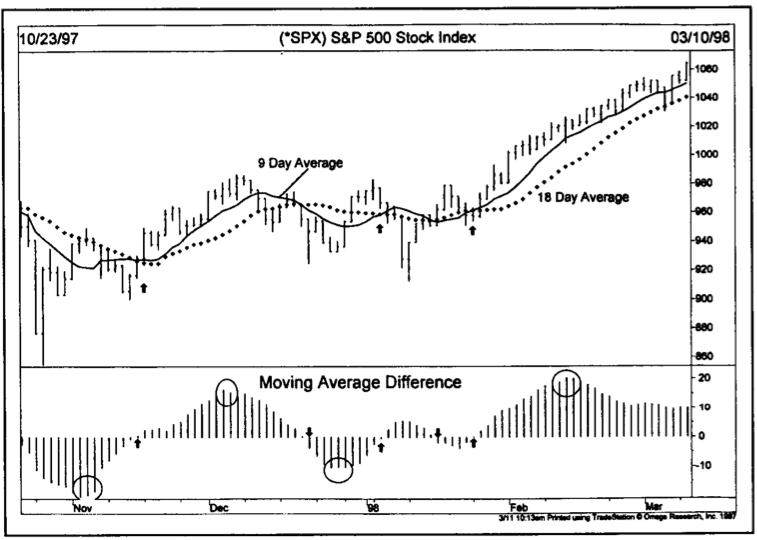
\includegraphics[width=0.8\textwidth]{graphics/fingrundlagen/macd.png}
	\caption[9,18 MACD-Histogramm]{9,18 MACD-Histogramm am Beispiel des S\&P 500 \cite{murphy-technische}}
	\label{fig:macd}
\end{figure}

%%%%%%%%%%%%%%%%%%%%%%%%%%%%%%%%%%%%%%%
\subsubsection{AMA}

Ein Problem des \gls{ema} ist es, die bestm�gliche L�nge zu w�hlen, um einen m�glichst aussagekr�ftigen Durchschnitt zu erhalten. Perry Kaufman schl�gt eine variable L�nge als L�sung des Problems vor. Dabei wird der Gl�ttungsfaktor eines \gls{ema} anhand der Volatilit�t des Preises der letzten $n$ Perioden bestimmt. Der resultierende Indikator wird folglich \gls{ama} genannt. \cite{murphy-technische}

Kaufman bestimmt die Volatilit�t durch eine \gls{er}, die berechnet wird, indem die absolute Gesamtpreisbewegung, i.e. Preis am Ende der Periode abz�glich des Preises am Beginn, durch die Summe der absoluten Preisbewegungen in einer Periode dividiert wird. Aufgrund der \gls{er} und zwei gegebenen L�ngen ($\alpha$ zwischen 0 und 1) wird nun ein tats�chlicher \gls{sf} berechnet. Dieser sollte zwischen den beiden gegebenen Werten liegen, was jedoch nur dann immer der Fall ist, wenn in der Berechnung des \gls{sf} $1$, nicht $2$ als Exponent gew�hlt wird.

\begin{equation}
	\label{Efficiency Ratio}
	ER = (\textrm{Gesamtpreisbewegung}) / (\textrm{Summe der Bewegungen pro Bar})
\end{equation}

\begin{equation}
	\label{Adaptive Moving Average - Smoothing Factor}
	SF = (ER * (SF_S - SF_L) + SF_L)^2
\end{equation}

\begin{equation}
	\label{Adaptive Moving Average}
	AMA_t = SF * P_{t} + (1 - SF) * AMA_{t-1}
\end{equation}

Dabei ist $SF_S$ der schnelle Smoothing Factor und $SF_L$ der langsame, zwischen denen das Ergebnis $SF$ abh�ngig von der $ER$ liegen soll.
Der Exponent kann als Abwandlung des Indikators auch ver�ndert werden, beispielsweise auf $1$, wenn der resultierende Durchschnitt genau im angegebenen Bereich liegen soll, oder auch auf $0.75$, falls konservativere Durchschnitte erw�nscht sind. \cite{kaufman_systems} \cite{ama_whs}

%%%%%%%%%%%%%%%%%%%%%%%%%%%%%%%%%%%%%%%
\subsubsection{Lineare Regression}

Um aus Zeitreihen einen allgemeinen Trend erkennen zu k�nnen, wird h�ufig eine lineare Regression durchgef�hrt. Dabei wird eine Gerade so gelegt, dass alle Punkte so nahe wie m�glich an
der Geraden liegen, wobei alle Punkte gleich stark gewichtet werden und auch m�glichst gleich weit entfernt liegen sollen. Zur Abstandsmessung werden die quadrierten y-Abst�nde zwischen Gerade und Preis herangezogen, damit gr��ere Abst�nde st�rker gewichtet werden als kleine. Die Gerade wird nun so gelegt, dass diese Summe der quadratischen Abst�nde m�glichst klein ist.

Das Minimum der folgenden Funktion der quadratischen Abst�nde muss durch partielles Differenzieren gefunden werden.

\begin{equation}
	\label{Funktion der quadratischen Abst�nde}
	F(k,d) = \sum\limits{i=1}{n}{{k*x_i + d - y_i}^2}
\end{equation}

Dadurch erh�lt man $k$ und $d$ der Regressionsgeraden. In der praktischen Anwendung ist meist besonders die Steigung $k$ der Geraden relevant.
Wird die Anzahl an historischen Preisen variiert, erh�lt man so Richtung und St�rke verschieden langer Trends.

%%%%%%%%%%%%%%%%%%%%%%%%%%%%%%%%%%%%%%%
\subsubsection{Average Directional Index}\label{subsection:adx}

Der \gls{adx} ist ein Indikator, der es auf einfache Weise erm�glicht, die St�rke eines Trends zu bestimmen, jedoch nicht, ob es sich um einen Aufw�rts- oder Abw�rtstrend handelt. Er wurde Ende der Siebziger von Welles Wilder entwickelt, der u.a. auch f�r den RSI (s. \ref{subsubsection:rsi}) verantwortlich ist. Der \gls{adx} ist ein Indikator, der sich aus der True Range (TR) und den Directional Movement-Indikatoren $DM_+$ und $DM_-$ zusammensetzt. Alle zusammen werden auch als Directional System bezeichnet. \cite{atr_whs} \cite{elder_living}

Der \gls{adx} wird in 5 Schritten berechnet.

\begin{enumerate}
	\item{Directional Movement ($DM_+$, $DM_-$) berechnen\\
		Directional Movement bezeichnet die Spanne, in der sich der Preis in der aktuellen Periode �ber oder unter der Preisspanne der letzten Periode bewegt hat.
		$DM_+$ ist dabei die Spanne dar�ber, $DM_-$ jene darunter. Der $DM$ ist dabei immer positiv, es wird also der Betrag der Differenz verwendet. (siehe Abbildung \ref{fig:dm})}
	\item{True Range ($TR$) berechnen\\
		Die True Range soll die tats�chliche Preisbewegung abbilden, also auch Bewegungen zwischen Perioden, bei denen Close- und Open-Preise
		nicht ident sind. Daf�r wird f�r die $TR$ immer der gr��te der folgenden 3 Werte herangezogen, die sich aufgrund von Preisen des aktuellen und 
		vorhergehenden Bars berechnet.
		\begin{enumerate}
			\item{$\left|\textrm{Aktuelles Hoch} - \textrm{Aktuelles Tief}\right|$}
			\item{$\left|\textrm{Aktuelles Hoch} - \textrm{Vorheriges Tief}\right|$}
			\item{$\left|\textrm{Aktuelles Tief} - \textrm{Vorheriges Tief}\right|$}
		\end{enumerate}}
	\item{Directional Indicators ($DI_+$, $DI_-$) berechnen\\
		 Die Directional Indicators sind das Verh�ltnis der Trendbewegung zur True Range, es gilt also:\\
		\begin{equation}
			DI_+ = \frac{DM_+}{TR}
		\end{equation}
		\begin{equation}
			DI_- = \frac{DM_-}{TR}
		\end{equation}}
	\item{Directional Indicators gl�tten\\
		Die Directional Indicators ($DI_{n+}$ und $DI_{n-}$) erh�lt man, indem die Directional Indicators ($DI_+$, $DI_-$) mit einem \gls{ma} gegl�ttet werden,
		wof�r in der Regel ein \gls{ema} verwendet wird. Die L�nge des verwendeten \gls{ma} ist dabei auf die Tradingstrategie anzupassen.
		$DI_{n+}$ und $DI_{n-}$ sind bereits f�r ein Handelssystem geeignet, da sie das Verh�ltnis von relativer Trendbewegung zur True Range gegl�ttet angeben.
		Aufgrund der Kreuzung der beiden Indikatoren k�nnen so auch Kauf- und Verkauf-Signale gegeben werden.}
	\item{$ADX$ berechnen\\
		Der \gls{adx} ist nun die nochmals gegl�ttete Differenz zwischen $DI_{n+}$ und $DI_{n-}$ und wird wie folgt berechnet:\\
		\begin{equation}
			ADX = EMA(\frac{DI_{n+} - DI_{n-}}{DI_{n+} + DI_{n-}})
		\end{equation}}
\end{enumerate} 

% V: Directional Movement Graph
\begin{figure}
	\centering
		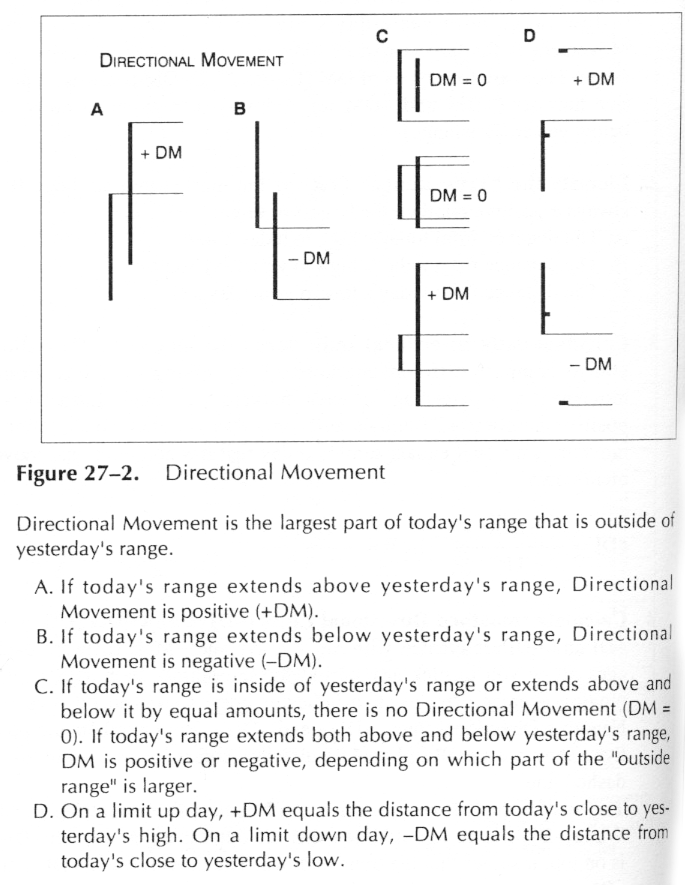
\includegraphics[width=0.8\textwidth]{graphics/fingrundlagen/dm.png}
	\caption[Berechnung des Directional Movement]{Berechnung des Directional Movement \cite{elder_living}}
	\label{fig:dm}
\end{figure}

Der \gls{adx} ist hilfreich, indem er anzeigt, ob sich der Markt in einer Trendphase befindet, in der Handelssysteme, die auf Trendfolgesystemen basieren, gut funktionieren, oder in einer Seitw�rtsphase,
in der sich andere Systeme eher rentieren. (z.B. Fading, siehe \ref{subsection:fading})  \cite{elder_living}

%%%%%%%%%%%%%%%%%%%%%%%%%%%%%%%%%%%%%%%
\subsubsection{Momentum}

Das Momentum ist ein Oszillator, der die Kurssteigung �ber einen gewissen Zeitraum angibt. Aus der Differenz des Preises zum Zeitpunkt $t$ und des Preises vor $n$ Perioden ergibt sich eine einfach interpretierbare Anzeige f�r die St�rke eines Trends. Aus einem 10-Tage-Momentum ist ablesbar, ob der Kurs aktuell h�her notiert als noch vor 10 Tagen. Wenn das Momentum negativ ist und ansteigt, ist ersichtlich, dass die St�rke eines aktuellen Abw�rtstrends abnimmt, wobei der Trend immer noch abw�rts gerichtet sein kann, er wird nur nicht mehr st�rker. Erst bei einem positiven Wert des Momentum ist ein Aufw�rtstrend zu erkennen.
Der gro�e Vorteil dieses Indikators liegt in der Fr�hzeitigkeit seiner Anzeige. Bevor sich der Trend umkehrt, zeigt der Momentum-Oszillator aufgrund der abnehmenden St�rke des aktuellen Trends bereits an, dass ein Trendwechsel bevorstehen k�nnte. Ein Problem des Momentum ist, dass die Werte absolut berechnet werden und dadurch die Schwankungsbreite abh�ngig vom betrachteten Kurs stark variieren kann. Die gleiche Berechnung auf relativer Basis wird nicht Momentum, sondern Rate-of-Change genannt.\\

Der Momentum-Indikator berechnet sich nach folgender Formel:

\begin{equation}
	\label{Momentum}
	M_t = P_t - P_{t-n}
\end{equation}
\cite{elder_living}

\begin{figure}
	\centering
		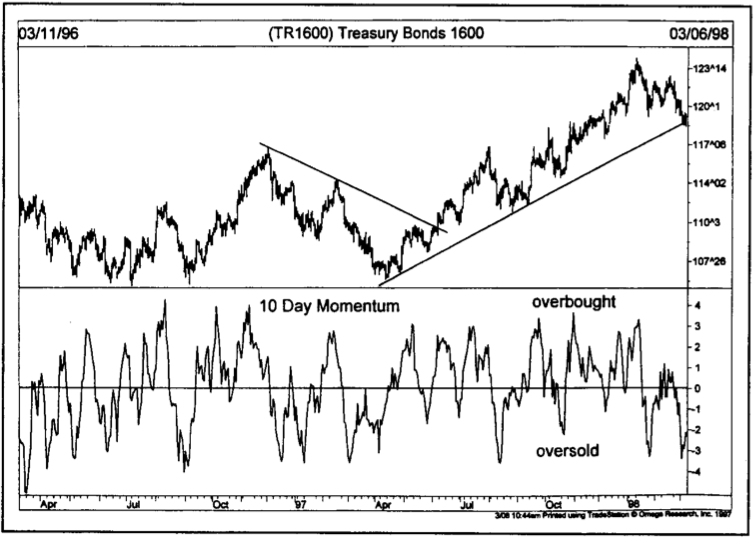
\includegraphics[width=0.8\textwidth]{graphics/fingrundlagen/momentum.png}
	\caption[10-Tage Momentum]{10-Tage Momentum, der �berkauft- und �berverkauft-Level anzeigt. \cite{murphy-technische}}
	\label{fig:momentum}
\end{figure}

%%%%%%%%%%%%%%%%%%%%%%%%%%%%%%%%%%%%%%%
\subsubsection{Relative Strength Indicator} \label{subsubsection:rsi}

Der \gls{rsi} gibt �hnliche Informationen wie das Momentum, schafft aber Abhilfe bei einigen Schwachstellen. Beispielsweise gibt es beim Momentum keine maximale Unter- und Obergrenze, wodurch es schwierig ist festzustellen, ob es sich momentan um eine Extremsituation handelt oder nicht. Der \gls{rsi} bewegt sich hingegen immer zwischen 0 und 100.
Eine wesentlich schwerwiegendere Schwachstelle des Momentums ist aber seine absolute Abh�ngigkeit von dem Kurs vor genau $n$ Zeitperioden. Sollte der Kurs zu der Zeit ein Hoch oder Tief erreicht haben, hat dies Auswirkungen auf das aktuelle Momentum, selbst wenn sich der aktuelle Kurs gar nicht oder nur kaum ver�ndert.\\

Der \gls{rsi} wird aus dem Durchschnitt der Schlusskurse von $n$ Tagen mit steigenden Kursen berechnet, dividiert durch den Durchschnitt der Schlusskurse von $n$ Tagen mit fallenden Kursen.\\

\begin{equation}
	\label{RS Up}
	RS_{Up} = \frac{\sum\limits_{i=0}^{n-1}{max(P_{t-i} - P_{t-i-1} ; 0)}}{n}
\end{equation}

\begin{equation}
	\label{RS Down}
	RS_{Down} = \frac{-\sum\limits_{i=0}^{n-1}{min(P_{t-i} - P_{t-i-1} ; 0)}}{n}
\end{equation}

Damit der \gls{rsi} immer zwischen 0 und 100 schwankt, kann nicht einfach $RS_{Up} / RS_{Down}$ berechnet werden, sondern es wird eine Normalisierung vorgenommen, die nichts an dem Aussehen
der \gls{rsi}-Kurve ver�ndert, sondern nur am Wertebereich.

\begin{equation}
	\label{RSI}
	RSI = \frac{RS_{Up}}{RS_{Up} + RS_{Down}}
\end{equation}

Der Erfinder sah urspr�nglich eine Zeitperiode von $n = 14$ Tagen vor, wobei aber f�r unterschiedliche Volatilit�t auch andere Parameter gew�hlt werden k�nnen. Interessant ist der \gls{rsi}, wenn er im Vorhinein festgelegte Level �berschreitet. Diese sind standardm��ig bei 70 und 30 f�r die �berkauft- und �berverkauft-Level, k�nnen aber beispielsweise als Anpassung f�r Bullenm�rkte auf 80 oder f�r B�renm�rkte auf 20 festgelegt werden.\cite{elder_living}

\begin{figure}
	\centering
		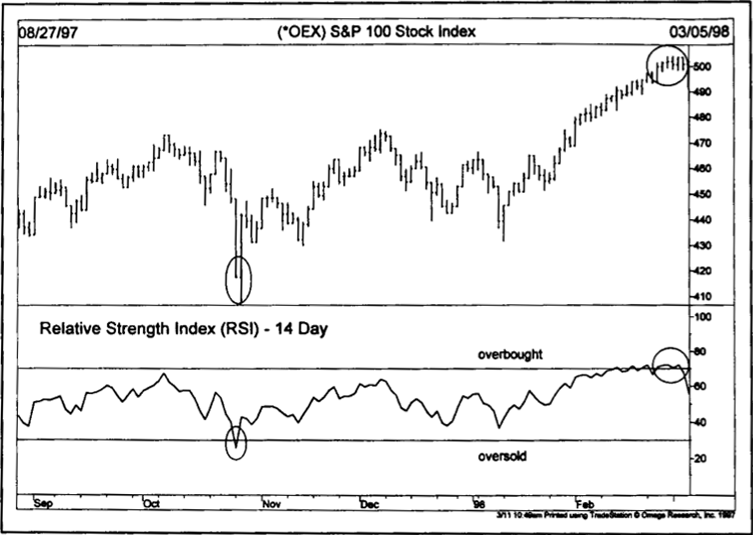
\includegraphics[width=0.8\textwidth]{graphics/fingrundlagen/rsi.png}
	\caption[14-Tage RSI]{14-Tage RSI am Beispiel des S\&P 100 \cite{murphy-technische}}
	\label{fig:rsi}
\end{figure}

%%%%%%%%%%%%%%%%%%%%%%%%%%%%%%%%%%%%%%%
\subsubsection{Prozentb�nder}

Prozentb�nder sind eine andere M�glichkeit, Nachhaltigkeit bzw. �berkauft- oder �berverkauft-Level festzustellen. Dazu wird ein \gls{ma} um einen festgelegten Prozentwert nach unten und oben verschoben, so dass ein Kanal bzw. ein Band entsteht, in dem der Kurs die meiste Zeit verl�uft. Wenn der Kurs �ber dem oberen Band notiert, wird dieser meist als �berkauft angesehen, da er im Vergleich zum Durchschnitt sehr schnell gestiegen ist. Um wie viel Prozent die B�nder nach oben und unten verschoben werden, h�ngt von der L�nge des \gls{ma} und somit dem Tradingzeitraum ab. Oft gebraucht werden 3\%-B�nder und eine 21-Tage-Linie oder 10\%-B�nder mit einem 40-Wochen-\gls{ma}.

%%%%%%%%%%%%%%%%%%%%%%%%%%%%%%%%%%%%%%%
\subsubsection{Bollinger B�nder}

Die Bollinger-B�nder, entwickelt von John Bollinger, sind ein �hnlicher Indikator wie die Prozentb�nder. Es wird ebenso ein Bereich oberhalb und unterhalb des \gls{ma} aufgespannt, aber anstatt ihn einfach um einen fixen Prozentwert zu verschieben, wird die Durchschnittslinie um die \emph{Doppelte Standardabweichung}, die meist auf L�nge des \gls{ma} berechnet wird, nach oben und nach unten verschoben.\\

Dabei dienen die B�nder meist als Kursziele, so dass beim Ansteigen des Kurses vom unteren Bollinger-Band das obere als Ziel angenommen wird. Diese Strategie wird auch als "`Fading"' bezeichnet und ist nur in Seitw�rtsphasen gewinnbringend, da der Preis w�hrend starken Trends lange Zeit entlang dem oberen oder unteren Rand des Bandes verlaufen kann. Die Breite der B�nder zeigt die Volatilit�t des Kurses an, da bei geringer Volatilit�t die Standardabweichung ebenfalls sinkt, ergo werden die B�nder schm�ler. Verschm�lern sich die B�nder in relativ kurzer Zeit, kann meist mit einem Ausbruch und einsetzendem Trend gerechnet werden. Bollinger B�nder k�nnen insgesamt sehr vielseitig eingesetzt werden, nicht nur in Seitw�rtsphasen, es existieren auch unterschiedliche Interpretations-Varianten.

\begin{figure}
	\centering
		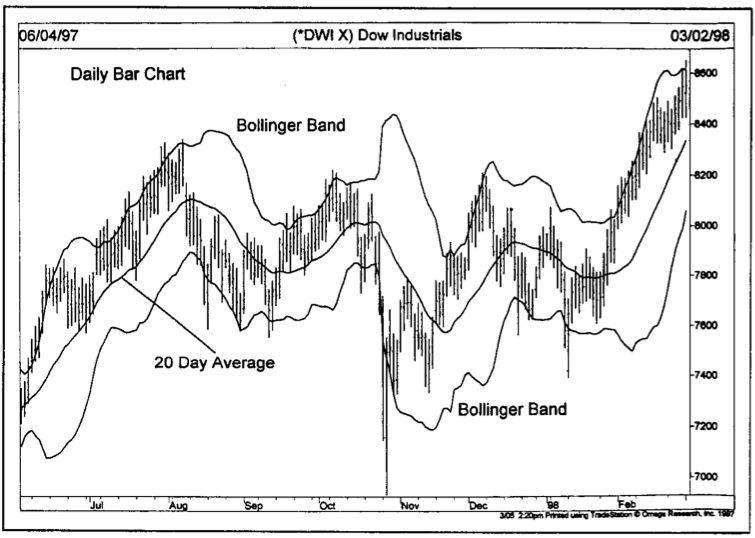
\includegraphics[width=0.8\textwidth]{graphics/fingrundlagen/bollinger.png}
	\caption[20-Tage Bollinger B�nder]{20-Tage Bollinger B�nder mit doppelter Standardabweichung am Beispiel des Dow Jones \cite{murphy-technische}}
	\label{fig:bollinger}
\end{figure}

%%%%%%%%%%%%%%%%%%%%%%%%%%%%%%%%%%%%%%%
\subsubsection{Pivot Points}

Pivot Points sind eine sehr h�ufig genutzte Variante zur Berechnung von horizontalen Support- und Resistance-Leveln. Dazu werden jeweils f�r eine Periode die Preisbewegungen der vorherigen Periode als Berechnungsgrundlage herangezogen. Als erstes wird der Typical Price (TP) der letzten Periode wie folgt berechnet.

\begin{equation}
TP = \frac{High+Low+Close}{3}
\end{equation}

Dieser wird als auch als Haupt-Pivot-Point bezeichnet, da von ihm ausgehend alle Unterst�tzungs- und Widerstandslevel festgelegt werden. Zur Berechnung verwendet werden immer die Daten aus der letzten Periode. Es werden zwei Level sowohl von Support- ($SL_1$ und $SL_2$) als auch von Resistance-Level ($RL_1$ und $RL_2$) berechnet, die je nach Marktsituation f�r unterschiedliche Zwecke ausgew�hlt werden k�nnen.

\begin{equation}
SL_1 = 2*TP - High
\end{equation} 

\begin{equation}
SL_2 = TP - (High - Low)
\end{equation} 

\begin{equation}
RL_1 = 2*TP - Low
\end{equation} 

\begin{equation}
RL_2 = TP + (High - Low)
\end{equation} 

\cite{tradimo_pivot_points}
% !TEX root = ../../Noctua_Diplomarbeit.tex

\subsection{Handelsstrategien mit MAs} \label{subsection:mastrategie}

Eine simples Tradingmodell basiert auf einer einfachen �berkreuzung eines \gls{ma} �ber den Preis. Es wird dabei angenommen, dass ein Aufw�rtstrend eingesetzt hat, wenn der Preis �ber den \gls{ma} steigt, da der Kurs begonnen hat, schneller als der Durchschnitt zu steigen. Umgekehrt wird angenommen, dass bei einem Abfall des Kurses unter den \gls{ma} ein Abw�rtstrend folgt und daher wird ein Short-Signal generiert. Eine zus�tzliche Sicherheit ist gegeben, wenn der \gls{ma} selbst in die erwartete Kursrichtung dreht. (siehe Abbildung \ref{fig:double_cross})

\begin{figure}
	\centering
		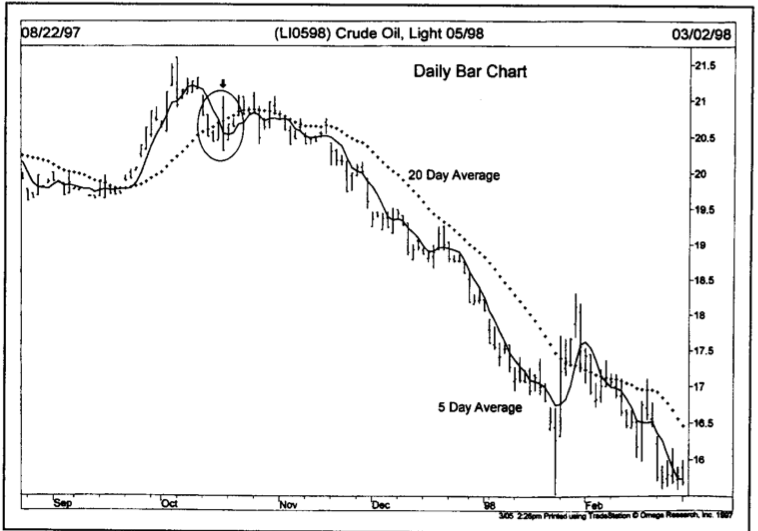
\includegraphics[width=0.8\textwidth]{graphics/fingrundlagen/double_cross.png}
	\caption[5,20 Double Cross Trading-System]{5,20 Double Cross Trading-System \cite{murphy-technische}}
	\label{fig:double_cross}
\end{figure}

Dieser simple Algorithmus hat einige Nachteile. Es wird zu jedem Zeitpunkt ein Signal gegeben, was bedeutet, dass immer entweder eine Long- oder eine Short-Position gehalten wird. Au�erdem verliert diese Strategie bei langen \glspl{ma} nach der Trendumkehr wieder viel vom Gewinn, da das Gegensignal erst sp�t generiert wird. Kurze \glspl{ma} erzeugen im Gegensatz dazu oft Fehlsignale.\\

Eine h�ufiger verwendete Variante zur Signalgenerierung mit \glspl{ma} wird \emph{Double Crossover Method} genannt. Dabei kommen zwei unterschiedlich lange \glspl{ma} zum Einsatz, wobei ein Signal erzeugt wird, wenn sich beide schneiden. Kreuzt der kurze \gls{ma} den l�ngeren, entsteht ein Kaufsignal, auch \emph{Golden Cross} genannt, und vice versa. Diese Variante erzeugt weniger Fehlsignale als die direkte Verwendung des Preises, hinkt dem Markt daf�r aber auch st�rker hinterher. Die L�nge der Durchschnitte h�ngt wie immer sowohl vom Handelszeitraum und der gew�nschten Signalanzahl als auch vom Markt ab.

Dieses System kann noch um einen weiteren \gls{ma} erweitert werden. Der Einsatz dreier Durchschnitte, oder \emph{Triple Crossover Method}, verfeinert die Signalgenerierung nochmals. Ein beginnender Aufw�rtstrend ist dann vorhanden, wenn der kurze \gls{ma} �ber dem mittleren liegt. Ein vollst�ndiges Kaufsignal entsteht, sobald der kurze �ber dem mittleren, und jener wiederum �ber dem langen \gls{ma} notiert. Eine umgekehrte Anordnung ist als Verkaufssignal anzusehen. Auf diese Art kann beispielsweise bei unklaren Signalen eine Neutralstellung (i.e. keine Aktien im Portfolio) eingenommen werden oder die Market-Exposure (i.e. Anzahl der Aktien) reduziert werden (siehe Abbildung \ref{fig:triple_cross}).
Normalerweise werden f�r solche Systeme \glspl{sma} verwendet, wobei aber besonders bei einem Double Cross\-over System auch die Anwendung eines \gls{ema},  \gls{dema} oder sogar \gls{tema} m�glich ist.

\begin{figure}
	\centering
		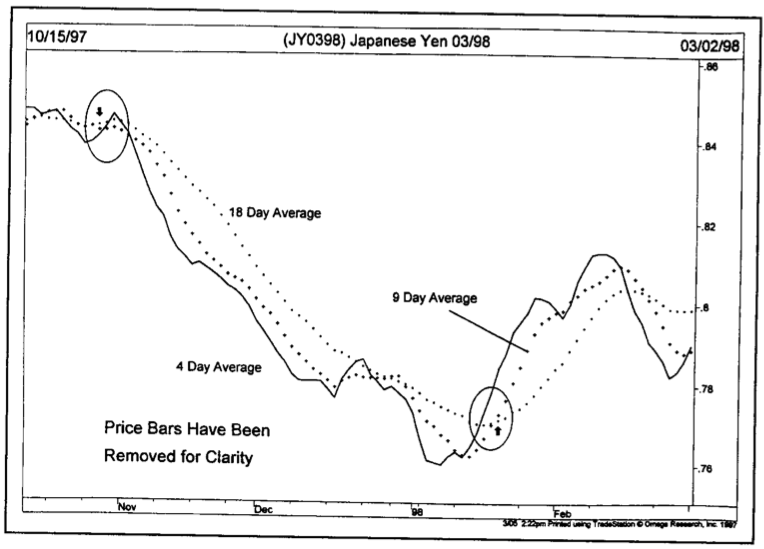
\includegraphics[width=0.8\textwidth]{graphics/fingrundlagen/triple_cross.png}
	\caption[4,9,18 Triple Cross Trading-System]{4,9,18 Triple Cross Trading-System \cite{murphy-technische}}
	\label{fig:triple_cross}
\end{figure}

\subsection{Fading-Strategie mit Bollinger B�ndern} \label{subsection:fading}

Seitw�rtsphasen zeichnen sich dadurch aus, dass der Preis mit einer gewissen Schwankungsbreite tendenziell weder steigt noch sinkt. Bollinger B�nder sind hervorragend daf�r geeignet, diese Schwankungsbreite statistisch abzubilden, da sie um ein Vielfaches der Standardabweichung (normalerweise der doppelten) des Durchschnitts nach oben und unten versetzt liegen. Um in dieser Situation Gewinn zu erzielen, w�re es daher vorteilhaft, dann zu kaufen, wenn der Preis nahe dem unteren Bollinger Band nach oben dreht und umgekehrt, wenn der Preis nahe dem oberen Bollinger Band nach unten dreht, zu verkaufen --- kurz gesagt, tief kaufen und hoch verkaufen. In l�ngeren Seitw�rtsphasen l�sst sich mit dieser Strategie gut ein Gewinn erzielen. Wenn die Bewegung jedoch recht schnell wieder einen Trend ausformt, muss dies schnell erkannt werden, um nicht zu viel des bereits erzielten Gewinns wieder zu verlieren. Anzeichen f�r einen einsetzenden Trend k�nnen z.B. kontrahierende Bollinger B�nder oder ein niedriger ADX-Wert sein.

% Alle Indikatoren beschreiben
% Quellen recherchieren
% Formel, wo m�glich
% Interpretation

\section{.NET-Framework}

% Was ist .NET
\subsection{Allgemein}

.NET ist ein Framework der Firma Microsoft, das eine Vielfalt an Sprachbibliotheken f�r eine gro�e Palette an Programmiersprachen zur Verf�gung stellt. Fr�her arbeiteten alle Programmiersprachen von Microsoft, wie bspw. C++, mit der WinAPI-32. Nun wurde dieses \gls{api} mit .NET durch ein sprachenunabh�ngiges, weitaus umfangreicheres Framework ersetzt. \cite{visualcsharp}\\
\\
Insgesamt wird die Nutzung des .NET-Frameworks von �ber 30 Programmiersprachen unterst�tzt. Die Richtlinien die eine Sprache einhalten muss, um als .NET-konform angesehen werden zu k�nnen, sind von Microsoft als \gls{cls} definiert worden. Zu den ber�hmtesten Vertretern solcher Sprachen Z�hlen C\#, F\#, Visual Basic .NET (VB.NET) und C++. \cite{visualcsharp}\\
\\
Zu den wichtigsten Features des .NET-Frameworks z�hlen die folgenden:
\begin{itemize}
\item \textbf{Objektorientierung} \\
	Das .NET-Framework ist zu 100\% objektbasiert. Das bedeutet, jegliche Elemente, sogar einfache Datentypen wie bspw. Integer, lassen sich auf Objekte zur�ckf�hren. Ja sogar die internen Zugriffe des Frameworks auf das darunterliegende Betriebssystem sind in Klassen gekapselt.
\item \textbf{Plattformunabh�ngigkeit} \\
	Anwendungen, die das .NET-Framework benutzen, werden �hnlich der \gls{jvm} erst zur Laufzeit in Maschinencode umgewandelt. Weiters ist die Spezifikation der von Microsoft benutzten Laufzeitumgebung, der sog. \gls{clr}, offen zug�nglich. Dadurch verlangt die Nutzung von .NET-Anwendungen also eine solche Umgebung, diese kann allerdings auch auf Plattformen portiert werden, die nicht Windows hei�en. So gibt es neben der propriet�ren Windows-Implementierung des .NET-Frameworks von Microsoft bspw. auch das \inline{Mono}-Projekt, mit dem .NET bereits erfolgreich auf Linux portiert werden konnte.
\item \textbf{Sprachenunabh�ngigkeit} \\
	Alle Komponenten des .NET-Frameworks k�nnen von jeder unterst�tzten Sprache problemlos verwendet werden. Das .NET-Framwork erm�glicht aber auch die Nutzung aller, in einer .NET-konformen Programmiersprache geschriebener Komponenten, in jeder anderen .NET-konformen Programmiersprache. So k�nnen zum Beispiel alle in C\# 2010 geschriebenen Klassen auch in F\# oder VB.NET genutzt und sogar abgeleitet werden.
\item \textbf{Speicherverwaltung} \\
	Die explizite Freigabe von nicht mehr ben�tigtem Speicher hat in der Vergangenheit schon zu vielen Problemen gef�hrt. Daf�r wurde mit dem .NET-Framework ein \inline{Garbage Collector} eingef�hrt, der dem Programmierer diese Aufgabe automatisch abnimmt. 
\item \textbf{Weitergabe} \\
	Auch die Weitergabe konnte deutlich vereinfacht werden. So k�nnen auf .NET basierende Sprachen einfach in eine .EXE- oder .\gls{dll}-Datei kompiliert und von jedem beliebigen Ordner aus ausgef�hrt werden. Eine .EXE-Datei ist dabei eine direkt ausf�hrbare Datei, deren Code bereits in einzelne Bytes umgewandelt wurde. \gls{dll}-Bibliotheken werden im folgenden Punkt erl�utert. \cite{visualcsharp}
\end{itemize}
% Was sind DLLs

\section{C\#-Grundlagen}

% Was ist C# (Microsoft)
% objektorientiert
\subsection{Allgemein}

Die Programmiersprache C\# wurde von der Firma Microsoft entwickelt und gilt als einer der wichtigsten Sprachen, die das .NET-Framework benutzen. C\# ist eine objektorientierte Programmiersprache mit einer fundamentalen Sprachsyntax. Mit diesen Eigenschaften eignet sie sich auch perfekt f�r die Nutzung von .NET. \cite{visualcsharp}\\
\\
Die Sprachsyntax von C\# ist der von Java sehr �hnlich. C\# wurde erstmals mit dem Ziel entwickelt, eine bessere, funktionsreichere Sprache zu entwickeln, die Java abl�sen k�nnte, trotzdem allerdings dessen Vorteile nutzt. Auch die allgemeine Struktur einer Klasse sowie der Aufbau simpler Anweisungen (if, for, while, etc.) sind quasi ident zu ihren �quivalenten in Java. \cite{visualcsharp}\\
\\
Eine C\#-Anwendung kann grunds�tzlich als Konsolenanwendung oder mit einer graphischen Oberfl�che (\gls{gui}) ausgef�hrt werden. Zur Realisierung einer solchen \gls{gui} werden ebenfalls mehrere Mechanismen zur Verf�hung gestellt. Zum einen gibt es die mittlerweile veraltete direkte M�glichkeit der Realisierung mit WinForms, einer API, die direkt in die Sprache integriert ist. Zum anderen hat Microsoft die \gls{wpf} entwickelt, die im folgenden Abschnitt \ref{wpf} genauer erl�utert wird. \cite{visualcsharp} \\
\\
Im folgenden sollen nun alle wichtigen Technologien der Sprache C\# beschrieben werden, die im Zuge dieses Projektes zum Einsatz gekommen sind.
% WPF
	% MVVM
	% XAML-GUI
	% GUI-Bindung
\subsection{Windows Presentation Foundation} \label{wpf}

Mit Version 3.0 des .NET-Frameworks wurde wie bereits erw�hnt zus�tzlich zur altbew�hrten WinForms-Variante, eine neue Variante integriert um Benutzeroberfl�chen einfach zu implementieren. Diese hei�t \gls{wpf}. \cite{visualcsharp}\\
\\
Das wichtigste Merkmal von \gls{wpf} gegen�ber anderen Methoden zur \gls{gui}-Erstellung ist, dass bei \gls{wpf} die Programmlogik nach strengsten Richtlinien von der Beschreibung der Oberfl�che trennt. Diese Beschreibung der Oberfl�che erfolgt mittels einer speziellen Version der normalen \gls{xml}, der \gls{xaml}. Mit dieser Sprache werden alle \gls{gui}-Komponenten, erzeugt und in die entsprechende Position gebracht. Bei \gls{wpf} wird allerdings trotzdem auch eine \gls{api} f�r den Zugriff auf \gls{xaml}-\gls{gui}-Komponenten innerhalb der Programmlogik bereit gestellt. Bei der Erstellung eines \gls{wpf}-Projektes, bekommt man automatisch ein MainWindow.xaml-File. Ein solches \gls{xaml}-File das lediglich einen Button als \gls{gui} anzeigt, w�rde nun in etwa so aussehen: \cite{visualcsharp}\\
\\
\begin{verbatim}
<Window x:Class="Wpf1Application1.MainWindow"
    xmlns="http://schemas.microsoft.com/winfx/2006/xaml/presentation"
    xmlns:x="http://schemas.microsoft.com/winfx/2006/xaml"
    Title="MainWindow" Height="350" Width="525">
    <Grid>
    	<Button Name="button1">Button</Button>
    <\Grid>
</Window>
\end{verbatim}

Hierbei werden zuerst die n�tigen von Microsoft definierten \gls{xaml}-Namespaces angegeben. Anschlie�end werden ein Titel (der ganz oben im Fenster angezeigt wird) und die Gr��e des Fensters angegeben, dass sp�ter unseren Button beinhalten soll. Danach wird ein einfaches Grid-Layout mit einem Button mit dem Text "Button" gezeichnet. Ab Microsoft Visual Studio 2008, wird auch ein \gls{wpf}-\gls{gui}-Builder bei der Installation mitgegeben, mit dem man diese \gls{xaml}-Dateien einfach mit graphischer Oberfl�che erstellen kann. \cite{visualcsharp}\\
\\
Zu der MainWindow.xaml-Datei wird auch noch eine weitere Datei mit dem Namen MainWindow.xaml.cs erstellt. Diese wird auch als \textit{Code-Behind}-Datei bezeichnet und beinhaltet den Teil der Programmlogik der direkt mit der graphischen Oberfl�che verkn�pft ist. M�chte man also bspw. die Logik implementieren, die beschreibt was bei einem Klick auf den Button passiert, m�sste man dies in eben dieser MainWindow.xaml.cs-Datei durchf�hren. \cite{visualcsharp}

\subsection{MVVM}
Als \gls{mvvm} wird ein Entwicklungsmuster (Design-Pattern) verstanden, dass sehr oft in Verbindung mit der Implementierung von \gls{wpf}-Oberfl�chen eingesetzt wird. Dabei werden die einzelnen Aufgaben einer Anwendung mit graphischer Oberfl�che in drei Teile aufgeteilt. Es gibt nun ein View, ein Model und ein ViewModel. Deren Interaktion kann in der Abbildung \ref{fig:mvvm} sehr sch�n nachvollzogen werden. \cite{msdn-mvvm}\\

\begin{figure}[h]
	\centering
		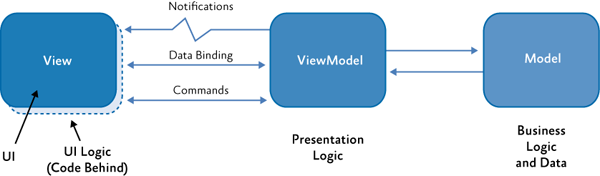
\includegraphics[width=0.90\textwidth]{graphics/grundlagen/mvvm.png}
	\caption{Aufbau von \gls{mvvm}}
	\label{fig:mvvm}
\end{figure}

Zuerst gibt es da also den View-Teil. Der View beschreibt das Aussehen der \gls{gui}. Im Optimalfall befindet sich um View ausschlie�lich ein Konstruktor mit einem Methodenaufruf InitializeComponents(), der die \gls{gui} �ber das \gls{xaml}-File aufbaut. Sollen allerdings komplexere graphisch aufwendigere Elemente oder Animationen in der grafischen Oberfl�che gezeichnet werden, kann diese Logik im View-Teil implementiert werden. Im View sollte allerdings nie Logik programmiert werden die man einem Unit-Testing unterziehen muss.\\ Wie der Abbildung \ref{fig:mvvm} entnommen werden kann, kommunziert der View nicht direkt, sondern ausschlie�lich �ber Commands, Notifications oder Data Binding mit dem ViewModel. Auf Commands wird hier nicht n�her eingegangen, Data Binding und Notifications k�nnen allerdings im folgenden Abschnitt \ref{databinding} gefunden werden. \cite{msdn-mvvm}\\
\\
Der ViewModel-Teil kapselt nun die Presentationslogik und die von der \gls{gui} ben�tigten Daten. Das ViewModel hat keinen direkten Zugriff auf den View und wei�t daher nichts �ber dessen Implementierung. Das ViewModel kann bspw. �ber die Verwaltung von Daten, die mittels Data Binding an den View weitergegeben werden mit diesem kommunizieren. Nebenbei bemerkt, m�ssen alle Daten die �ber Data Binding an den View weitergegeben werden sollen ausschlie�lich im ViewModel gespeichert werden. Das ViewModel beschreibt also welche Funktionalit�t die \gls{gui} anbieten soll und das View, wie diese angezeigt wird. Das ViewModel fungiert au�erdem quasi als Mittelmann zwischen dem View und dem Model und kann dabei bspw. noch die Daten aus dem Model so vereinfachen, dass der View diese leichter verarbeiten kann. \cite{msdn-mvvm}\\
\\
Das Model ist nun die eigentliche Gesch�fts- oder Programmlogik und die damit verbundenen allgemeinen Daten. Hierbei handelt es sich um eine ganz normale Gesch�ftslogik wie in anderen Anwendungen auch, nur dass noch einmal speziell Wert darauf gelegt werden sollte die einzelnen Codest�cke nicht Task-spezifisch zu implementieren, um die einzelnen St�ck sp�ter m�glicherweise an anderen Stellen wiederverwenden zu k�nnen. Au�erdem besteht das Model entgegen dem View und dem Viewmodel meist aus vielen einzelnen Model-Klassen, die alle mit dem selben ViewModel kommunizieren. M�chte das Model auch mit dem View interagieren gibt es auch hier die M�glichkeit Notifications zu benutzen.\cite{msdn-mvvm}

\subsection{Data Binding} \label{databinding}

Das Data Binding (auch: Datenbindung) erm�glicht \gls{gui}-Komponenten den Zugriff auf Daten, die sie anzeigen k�nnen. In WinForms war die Datenbindung auch schon integriert, lediglich war man mit den damaligen Methoden auf wenige Controls beschr�nkt. Mit \gls{wpf} ist man dies nun nicht mehr. Daten k�nnen hiermit n�mlich direkt aus einer der folgenden Datenquellen entnommen werden \cite{visualcsharp}:

\begin{itemize}
	\item ViewModel
	\item Eigenschaften anderer Komponenten
	\item \gls{xml}-Datei
	\item Collections
	\item Datenbanken
	\item etc.
\end{itemize} \cite{visualcsharp}

Zur Nutzung von Data Binding sind nun zwei Klassen wichtig, DataContext und Binding. Der DataContext ist die Datenquelle von der die Daten bezogen werden sollen. Dieser DataContext ist au�erdem ein Attribut jedes \gls{gui}-Elements und muss gesetzt werden, damit Bindungen funktionieren. M�chte man nun den DataContext setzen sollte man aber aufpassen und ihn im �bergeordneten Container (z.B. dem MainWindow) setzen, denn davon profitieren alle untergeordneten Komponenten dieses Conatiners und der DataContext muss nict �berall gesetzt werden. Das Binding-Objekt beschreibt nun die Binung zwischen einer Datenquelle und einer bindenden Komponente. Das Binding wird meist im \gls{xaml}-Code geschrieben, es besteht allerdings selbstverst�ndlich auch die M�glichkeit sie innerhalb des C\#-Codes zu erzeugen. \cite{visualcsharp}\\
\\
Das einfachste Beispiel f�r eine Bindung k�nnte nun in etwa so aussehen:

\begin{verbatim}
<Window x:Class="Wpf1Application1.MainWindow"
    xmlns="http://schemas.microsoft.com/winfx/2006/xaml/presentation"
    xmlns:x="http://schemas.microsoft.com/winfx/2006/xaml"
    Title="MainWindow" Height="350" Width="525">
    <Window.DataContext>
    	<local:MainViewModel x:Name="mainViewModel" />
    </Window.DataContext>
    <StackPanel>
    	<TextBox Name="txtOben" Height="50" FontSize="16"></TextBox>
    	<TextBox Name="txtUnten" Height="50" Background="AliceBlue" FontSize="16">
    		<Binding ElementName="txtOben" Path="Text" />
    	</TextBox>
    </StackPanel>
</Window>
\end{verbatim} \cite{visualcsharp}

Zuerst wird hier der \textit{DataContext} auf das ViewModel gesetzt. Dies w�re hier zwar noch nicht notwendig, da keine Bindung auf ein Property aus dem ViewModel erfolgt, es zeigt allerdings die angesprochene Funktionsweise und wird im n�chsten Beispiel von Bedeutung sein. Danach werden zwei \textit{TextBoxen} erstellt von denen die Text-Variable der unteren eine Bindung auf die Text-Variable der oberen besitzt. Dadurch wird der Text der unteren \textit{TextBox} automatisch an den Text der oberen \textit{TextBox} angepasst, falls sich dieser �ndert. Eine Bindung in dieser Art k�nnte aber auch auf jedes andere Attribute der \textit{TextBoxen} (z.B. Gr��e, Schriftart, etc.) angewendet werden. Dazu m�sste lediglich der \textit{Path} der Bindung ge�ndert werden. \cite{visualcsharp}\\
\\
Eine etwas kompliziertere Bindung ist die auf ein Property aus dem ViewModel. Dazu muss man zuerst im ViewModel ein Property erzeugen und dessen setter-Methode f�r die Nutzung von Notifications implementieren. Das Property, das die Lieblingsfarbe einer Person speichert, k�nnte dann in etwa so aussehen \cite{msdn-mvvm}:

\begin{verbatim}
public class MyViewModel : INotifyPropertyChanged
{
    private string favoriteColor;
    public event PropertyChangedEventHandler PropertyChanged;
    ...
    public string FavoriteColor
    {
        get { return this.favoriteColor; }
        set
        {
            if (value != this.favoriteColor)
            {
                this.favoriteColor = value;
                if (this.PropertyChanged != null)
                {
                    this.PropertyChanged(this,
                          new PropertyChangedEventArgs("FavoriteColor"));
                }
            }
        }
    }
}
\end{verbatim} \cite{msdn-mvvm}

Hierbei wird einfach eine globale Variable (\textit{favoriteColor}) mit einem Property (\textit{FavoriteColor}) versehen, das die setter-Methode so implementiert hat, dass ein \textit{PropertyChangedEvent} gesendet wird, sobald der Wert der Lieblingsfarbe ge�ndert wird. Dies ist notwendig, wenn man das Property an ein \gls{gui}-Element binden will, da sich das \gls{gui}-Element, sonst im Falle einer �nderung der Lieblingsfarbe nicht aktualisieren w�rde. M�chte man dieses Property nun im \gls{xaml}-Code an ein \gls{gui}-Element binden, muss man lediglich das Folgende schreiben:

\begin{verbatim}
<Window x:Class="Wpf1Application1.MainWindow"
    xmlns="http://schemas.microsoft.com/winfx/2006/xaml/presentation"
    xmlns:x="http://schemas.microsoft.com/winfx/2006/xaml"
    Title="MainWindow" Height="350" Width="525">
    <Window.DataContext>
    	<local:MainViewModel x:Name="mainViewModel" />
    </Window.DataContext>
    <StackPanel>
    	<TextBox Name="favoriteColorTextBox" Height="50" FontSize="16">
    		<Binding Path="FavoriteColor" />
    	</TextBox>
    </StackPanel>
</Window>
\end{verbatim}

Diesmal ist die Definition des ViewModels als \textit{DataContext} notwendig. Aus diesem wird n�mlich einfach in der Bindung das \textit{FavoriteColor}-Property aufgerufen. Schon steht zu jeder Zeit die aktuelle Lieblingsfarbe aus dem ViewModel in der \textit{TextBox}.
% Charting-Library (.NET)
\lstset{style=sharpc}
\subsection{Microsoft Chart Controls} \label{charting}

Die Microsoft Charts Controls Library ist eine sehr umfangreiche Bibliothek, die es erm�glicht in WinForms-Anwendungen oder auf Webseiten mit ASP.NET Charts und Diagramme zu zeichnen. Die M�glichkeiten sind derma�en umfangreich, dass es im Folgenden nur Sinn macht, die Funktionen zu erl�utern, die f�r die Darstellung finanzieller Charts erheblich sind. Zu den Hauptfeatures z�hlen daher \cite{msdn-charting}:

\begin{itemize}
\item \textbf{Charttypen} \\
	Es werden 35 verschiedene Charttypen unterst�tzt, dabei alles von normalen Liniencharts bis zu Bar- und Candlestick-Charts zur Darstellung von Aktiendaten.
\item \textbf{Skalierbarkeit} \\
	Es k�nnen unendlich viele Daten, Chart-Areas (Bereiche innerhalb eines Charts), Bemerkungen (z.B. Pfeile), etc. innerhalb eines Charts angezeigt werden. Daher k�nnen bspw. Aktiendaten und deren \glspl{ma} in einer ChartArea angezeigt werden. Zus�tzlich k�nnte man eine weitere ChartArea erg�nzen um bspw. einen \gls{macd}-Verlauf direkt unter den Aktiendaten zu zeichnen.
\item \textbf{Daten} \\
	Es werden Unmengen an M�glichkeiten zur Verwaltung der Daten innerhalb eines Charts, wie z.B. Data Binding, zur Verf�gung gestellt. Au�erdem k�nnen die Daten des Charts exportiert, oder zum Speichern serialisiert werden. 
\item \textbf{Aussehen} \\
	Weiters k�nnen sowohl zweidimensionale als auch dreidimensionale Charts erstellt werden, die alle sehr simpel und sch�n dargestellt werden. Die k�nnen zudem auch zur Laufzeit noch weiter manipuliert werden und die WinForms-Version bietet sogar M�glichkeiten zum interaktiven Zoomen und Scrollen f�r den User. (Auf Webseiten mit ASP.NET werden keine interaktiven Funktionen f�r den Benutzer der Website angeboten.) 
\end{itemize} \cite{msdn-charting}

\subsubsection{Nutzung mit WPF} \label{winformshost}

Leider ist momentan noch keine Version f�r die Verwendung mit \gls{wpf} erh�ltlich, man kann diese Einschr�nkung allerdings umgehen indem man einen sog. \textit{WinFormsHost} erstellt. Dies ist ein \gls{wpf}-\gls{gui}-Element, das WinForms-Elemente so kapselt, dass sie in \gls{wpf} genutzt werden k�nnen. Dieses Element mit einem \textit{MSChart} kann so erstellt werden:

\begin{lstlisting}[label=MSChart in einer WinFormsHost-Umgebung,caption=MSChart in einer WinFormsHost-Umgebung]
<WindowsFormsHost Name="WfHost" Grid.Row="0">
	<MSChart:Chart x:Name="MyWinformChart">
	    <MSChart:Chart.ChartAreas>
	        <MSChart:ChartArea Name="MainArea"/>
	    </MSChart:Chart.ChartAreas>
	</MSChart:Chart>
</WindowsFormsHost>
\end{lstlisting}

Hier wurde au�er dem primitiven \textit{MSChart} auch gleich eine \textit{ChartArea} hinzugef�gt. Eine \textit{ChartArea} ist ein Bereich innerhalb des Charts (hier der gesamte Bereich des Charts), in dem eine Funktion gezeichnet werden kann. Damit dieses WinFormsHost-Element allerdings funktioniert m�ssen f�r das gesamte \textit{Window} noch folgende Namespaces erg�nzt werden (diese Assemblies m�ssen nat�rlich auch als Verweis zum Projekt hinzugef�gt werden):

\begin{lstlisting}[label=Namespaces f�r MSChart und WinFormsHost,caption=Namespaces f�r MSChart und WinFormsHost]
xmlns:wf="clr-namespace:System.Windows.Forms;assembly=System.Windows.Forms"
xmlns:MSChart="clr-namespace:System.Windows.Forms.DataVisualization.Charting;assembly=System.Windows.Forms.DataVisualization"
xmlns:wfi="clr-namespace:System.Windows.Forms.Integration;assembly=WindowsFormsIntegration"
\end{lstlisting}

\subsubsection{Darstellung einfacher Graphen}

Nachdem eine leere \textit{ChartArea}, in die ein Graph gezeichnet werden kann, bereits im \gls{xaml} erzeugt wurde, muss man im C\#-Code nur noch das \textit{Chart} suchen, in das gezeichnet werden soll und eine \textit{Series} erstellen. In diese Series werden dann die Daten eingespeist, die gezeichnet werden soll. Wenn man nun auch noch einen Typ f�r den Graphen konfiguriert wird dieser auch schon in der \textit{ChartArea} angezeigt. Um bspw. eine Sinusfunktion darzustellen m�sste man nun folgenden Code schreiben: \cite{msdn-charting}

\begin{lstlisting}[label=Erstellung einer Series,caption=Erstellung einer Series]
//Lookup des bereits im XAMl-Code definierten Charts
Chart chart = this.FindName("MyWinformChart") as Chart;

//Erstellen der Series
Series sinus = new Series("Sinus");

//Berechnung einer Sinuskurve und speichern der
//errechneten Daten in die Series
for (double i = 0; i <= 7.5; i += 0.2)
	sinus.Points.AddXY(i, Math.Sin(i));

//Definieren des Zeichentyps als normale Linie
sinus.ChartType = SeriesChartType.FastLine;
 
// Hinzufuegen des Graphs zum Chart
chart.Series.Add(sinus);
\end{lstlisting} \cite{mschart-grundlagen}

In diesem Beispiel wurde jeder Punkt des Sinus einzeln berechnet und zur \textit{Series} hinzugef�gt. Dies k�nnte man nat�rlich auch mit jeder anderen Datenquelle wie zum Beispiel einer Liste machen, in dem man jeden Wert einzeln hinzuf�gt. \cite{msdn-charting}

\subsubsection{Finanzielle Berechnungen} \label{finfor}

Die Microsoft Chart Controls Library bietet allerdings nicht nur M�glichkeiten zur einfachen Darstellung von Daten. Denn sie beinhaltet ein Framework aus �ber 50 veschiedenen statistischen und finanziellen Formeln zur automatischen Berechnung und Darstellung spezieller Werte. \cite{msdn-charting}\\
\\
Die wichtigsten Formeln in der \textit{FinancialFormula}-Sammlung der MS Chart Controls sind:

\begin{itemize}
\item Bollinger B�nder
\item \gls{cci}
\item diverse \glspl{ma}
\item \gls{macd}
\end{itemize} \cite{msdn-charting}

Im Code w�rde der Einsatz von \textit{FinancialFormula} so aussehen:

\begin{lstlisting} [label=Berechnung eines WMA mit FinancialFormula,caption=Berechnung eines WMA mit FinancialFormula]
chart.DataManipulator.FinancialFormula(FinancialFormula.WeightedMovingAverage, 90, "Data", "FinFor");
\end{lstlisting} \cite{msdn-charting}

Dieser Aufruf erzeugt einen \gls{ma} der L�nge 90. Dazu holt er sich die Daten aus der Series ''\textit{Data}'', berechnet den \gls{ma} und schreibt die errechneten Daten in die \textit{Series FinFor}. Damit diese Berechnung m�glich ist muss die \textit{Series FinFor} bereits zuvor erzeugt und die \textit{Series Data} ebenfalls bereits zuvor erzeugt auch wirklich mit Daten gef�llt sein. \cite{msdn-charting}
% C# Tuples
\lstset{style=sharpc}
\subsection{C\# Tupel}

Ein Tupel ist prinzipiell eine Ansammlung von Werten. Dabei kann es beliebig viele Werte mit verschiedenen Datentypen haben. Eben diese Anzahl und die dazugeh�rigen Datentypen m�ssen allerdings schon im Vorhinein festgelegt werden, wenn das Tupel erzeugt wird. Ein \inline{Tuple} in C\# k�nnte bspw. so aussehen \cite{cs-tuple}:

\begin{lstlisting} [label=Erstellung eines Tuples,caption=Erstellung eines Tuples]
Tuple<int, bool> tuple = new Tuple<int, bool>(1, true);
\end{lstlisting}

Dabei handelt es sich um ein sehr einfaches \inline{Tuple}, das lediglich einen Integer-Wert zu einem dazugeh�rigen Boolean-Wert speichert. Ein \inline{Tuple} ist eine Klasse, in der direkt Werte gespeichert werden. Deshalb muss er einen separaten Ort im Heap allokieren. \cite{cs-tuple} Dies bedeutet, dass bspw. ein Tupel mit zwei Werten in der Erstellung wesentlich l�nger ben�tigt als ein \inline{KeyValuePair}, es aber sp�ter in der Nutzung eine deutlich h�here Performance aufweist. \cite{tuple-performance} Au�erdem k�nnen durch diese Tatsache die Datentypen der Felder des Tupels nach dessen Erstellung absolut nicht mehr ge�ndert werden, was das \inline{Tuple} eigentlich mehr einer \inline{struct} �hneln l�sst. \cite{cs-tuple}\\
\\
In der Praxis werden selten einzelne Tupel verwendet. Es ist allerdings oft von Vorteil eine Liste aus Tupeln zu erzeugen, wenn man quasi eine \inline{Map} (bzw. ein \inline{Dictionary}) mit mehreren Werten oder anderen Datentypen ben�tigt. So k�nnen z.B. Aktienpreis-Bars als Tupel aus einem \inline{TimeStamp} und Feldern f�r Open, High, Low und Close realisiert werden. Daraus kann dann eine Liste erstellt werden, um die Bars ad�quat speichern zu k�nnen.
% Speichern
\lstset{style=sharpc}
\subsection{Bin�re Serialisierung} \label{Binaere-Serialisierung}

Objekte in .NET-Sprachen sind grunds�tzlich fl�chtig, dass bedeutet das sie nach der Beendung und einem anschlie�enden Neustart der Anwendung nicht mehr vorhanden sind. Oft ben�tigen Entwickler allerdings die Funktion, solche Objekte zu persistieren, sie also nach einem Neustart der Applikation weiterhin verf�gbar zu machen. Dies kann durch bin�re Serialisierung erreicht werden. Bei diesem Verfahren k�nnen �ber einen sog. \textit{BinaryFormatter} alle als \textit{Serializable} gekennzeichneten Objekte und deren aktueller Zustand, sprich all deren Variablenwerte, in bin�ren Code umgewandelt werden. Dieser bin�re Code k�nnte bspw. in einer persistenten Datei, einer Datenbank oder einer Anwendungskonfigurationsdatei (Siehe \ref{akd}) gespeichert werden. Weiters k�nnte dieser serialisierte Bin�rcode eines Objektes auch leicht �ber das Netzwerk �bertragen werden, ohne dass die einzelnen Softwarekomponenten auf dem Weg des Objekts auch dessen Definition (Klasse) kennen m�ssen. \cite{visualcsharp}

\subsubsection{Anwendung}

Neben der einfachen Serialisierung mit dem \textit{BinaryFormatter}, bietet das .NET-Framework auch einen \textit{SoapFormatter} und einen \textit{XmlSerializer}. Der \textit{SoapFormatter} �bertr�gt den aktuellen Zustand eines Objekts nicht in ein bin�res, sondern in ein \gls{soap}-Format. Dieses wird bei der �bertragung von Daten �ber das Netzwerk mittels einer \gls{soap}-Verbindung ben�tigt, um Objekte �bertragen zu k�nnen. Der \textit{XmlSerializer} �bertr�gt die Daten des betroffenen Objekts in ein \gls{xml}-Format, um es als \gls{xml}-Datei abspeichern und ggf. sp�ter wieder auslesen zu k�nnen. Im folgenden werde ich allerdings nur auf den wichtigsten, den \textit{BinaryFormatter}, eingehen, der Objekte einfach in ein bin�res Format �berf�hrt und auf einen Stream legt. Dazu m�ssen lediglich alle globalen Variablen bzw. deren Werte in Bin�rcode umgewandelt und gespeichert werden. Methodendefinitionen, etc., m�ssen dabei nicht serialisiert werden, da zur Deserialisierung und anschlie�enden Nutzung des Objekts die Klassendefinition des Objekts ohnehin vorhanden sein muss. Die Serialisierung funktioniert wie folgt \cite{visualcsharp}:

\begin{lstlisting}[label=Serialisierung mit einem BinaryFormatter,caption=Serialisierung mit einem BinaryFormatter]
BinaryFormatter bFormatter = new BinaryFormatter();
bFormatter.Serialize(stream, object);
\end{lstlisting}

Dazu wird also zuerst ein neuer \textit{BinaryFormatter} initialisiert und anschlie�end die \textit{Serialize}-Methode aufgerufen. Der \textit{Serialize}-Methode muss dabei zuerst ein Stream �bergeben werden. Bei diesem Stream wird es sich meist um einen \textit{FileStream} handeln, der das umgewandelte Objekt auch sofort in eine Datei schreibt. Es kann allerdings bspw. auch ein Kommunikationsstream oder jede andere m�gliche Art von Streams, die vom Objekt \textit{Stream} erbt, �bergeben werden. Als zweiter Parameter kann jedes m�gliche Objekt, dessen Klasse von \textit{Object} erbt und mit dem \textit{Serializable()}-Attribut gekennzeichnet ist, �bergeben werden. Es kann hier aber auch bspw. eine Liste �bergeben werden, sofern sowohl die Liste selbst als auch all ihre gespeicherten Elemente das \textit{Serializable()}-Attribut besitzen. \cite{visualcsharp}\\
\\
Eine Klasse kann wie folgt bei der Deklaration mit dem \textit{Serializable()}-Attribut gekennzeichnet werden \cite{visualcsharp}:

\begin{lstlisting}[label=Markierung einer Klasse als Serializable,caption=Markierung einer Klasse als Serializable]
[Serializable()]
class Klasse{
	...
}
\end{lstlisting}

Dies ist lediglich die Markierung der Klasse �ber ein sog. Markup-Interface. Dadurch wird der Compiler dar�ber informiert, dass Objekte dieser Klasse keinen au�ergew�hnlich heiklen Inhalt beinhalten und somit bedenkenlos serialisiert werden d�rfen. Fehlt dieses Attribut, so wird eine \textit{SerializationException} ausgel�st. \cite{visualcsharp}\\
\\
M�chte man ein bereits serialisiertes Objekt aus dem Bin�rcode wieder auslesen und als Objekt speichern, ben�tigt man ebenfalls die Klasse \textit{BinaryFormatter} und dessen \textit{Deserialize}-Methode. Dieser muss nur der Stream �bergeben werden, der sich ohnehin mit seinem internen Zeiger auf einer Position befindet. Mit dem Aufruf der \textit{Deserialize}-Methode wird ab der aktuellen Zeigerposition das n�chste serialisierte Objekt gesucht, zur�ck in ein normales Objekt umgewandelt und als \textit{Object} zur�ckgegeben. Damit dieses \textit{Object} wieder als das urspr�ngliche erkannt wird und mit der richtigen Klassendefinition verkn�pft wird, muss es zus�tzlich noch auf den gew�nschten Typ gecastet werden. \cite{visualcsharp}

\begin{lstlisting}[label=Deserialisierung mit einem BinaryFormatter,caption=Deserialisierung mit einem BinaryFormatter]
BinaryFormatter bFormatter = new BinaryFormatter();
Object object = (Object) bFormatter.Deserialize(stream);
\end{lstlisting}

\subsection{Konfigurationsdateien}

Das .NET-Framework unterst�tzt die Nutzung vieler verschiedener Konfigurationsdateien. Diese Konfigurationsdateien beinhalten grunds�tzlich einfach nur Daten, die zur Laufzeit von der Anwendung ausgelesen werden k�nnen. Dadurch kann bspw. das Laufzeitverhalten der Anwendung komplett ver�ndert werden oder einfach nur ein einfach verwalteter Datenspeicher eingerichtet werden. Es gibt Anwendungskonfigurationsdateien, Herausgeberrichtliniendateien und die Maschienenkonfigurationsdatei, die beim Start der Anwendung auch in dieser Reihenfolge aufgerufen werden. Im folgenden wird allerdings lediglich auf die Anwendungskonfigurationsdateien eingegangen.  \cite{visualcsharp}

\subsubsection{Anwendungskonfigurationsdateien} \label{akd}

Eine Anwendungskonfigurationsdatei ist f�r die Ausf�hrung einer Anwendung optional. Ist sie allerdings vorhanden, so dient sie zur Verwaltung und Sicherung der Stammdaten der gesamten Anwendung im \gls{xml}-Format. Diese Datei befindet sich immer im Stammverzeichnis der Anwendung und ihr Name setzt sich aus dem Namen der Anwendung und dem Suffix \textit{.config} zusammen. Meist wird sie dazu verwendet, den aktuellen Zustand einer Anwendung, das bedeutet alle zur Laufzeit gesetzten Variablen, zu sichern, um sie sp�ter im selben Zustand neu starten zu k�nnen. Dazu werden meist alle wichtigen Daten beim Beenden der Applikation in die Anwendungskonfigurationsdatei gespeichert und beim Start der Anwendung erneut aus dieser ausgelesen. \cite{visualcsharp}\\
\\
Innerhalb der \gls{xml}-Datei in der \textit{<configuration>}-Sektion werden zur Verwaltung dieser Stammdaten vier verschiedene Code-Sektionen angeboten. \cite{visualcsharp}

\begin{itemize}
\item \textit{<configSections>} \\
	Diese Sektion beschreibt lediglich das Ausma� der beiden untergeordneten Sektionen \textit{<applicationSettings>} und \textit{<userSettings>}.
\item \textit{<applicationSettings>} \\
	Diese Sektion speichert alle Stammdaten, die f�r die gesamte Anwendung (und jeden Benutzer) g�ltig sein sollen.
\item \textit{<userSettings>} \\
	Diese Sektion erlaubt die Definition und Sicherung von Stammdaten der Anwendung, die immer nur f�r einen einzigen Benutzer g�ltig sind. Dies ist besonders f�r benutzerspezifische Einstellungen unentbehrlich.
\item \textit{<appSettings>} \\
	Diese Sektion bietet grunds�tzlich die selben Funktionen wie die Sektion \textit{<applicationSettings>}, kann jedoch aus dem Code der laufenden Anwendung heraus editiert werden. \cite{visualcsharp}
\end{itemize}

Da die manuelle Erstellung einer solchen Anwendungskonfigurationsdatei sehr kompliziert w�re und mit einem sehr gro�en Aufwand verbunden ist, hat Microsoft eine unterst�tzte Erstellungshilfe mit graphischer Oberfl�che in seine Entwicklungsumgebung Visual Studio integriert. Dazu m�ssen nur die Project-Properties des entsprechenden Projekts ge�ffnet und hier der Tab "`Einstellungen"' gew�hlt werden. Dadurch kommt man zu der Oberfl�che aus Abbildung \ref{fig:akdErstellung}. \cite{visualcsharp}

\begin{figure}[h]
	\centering
		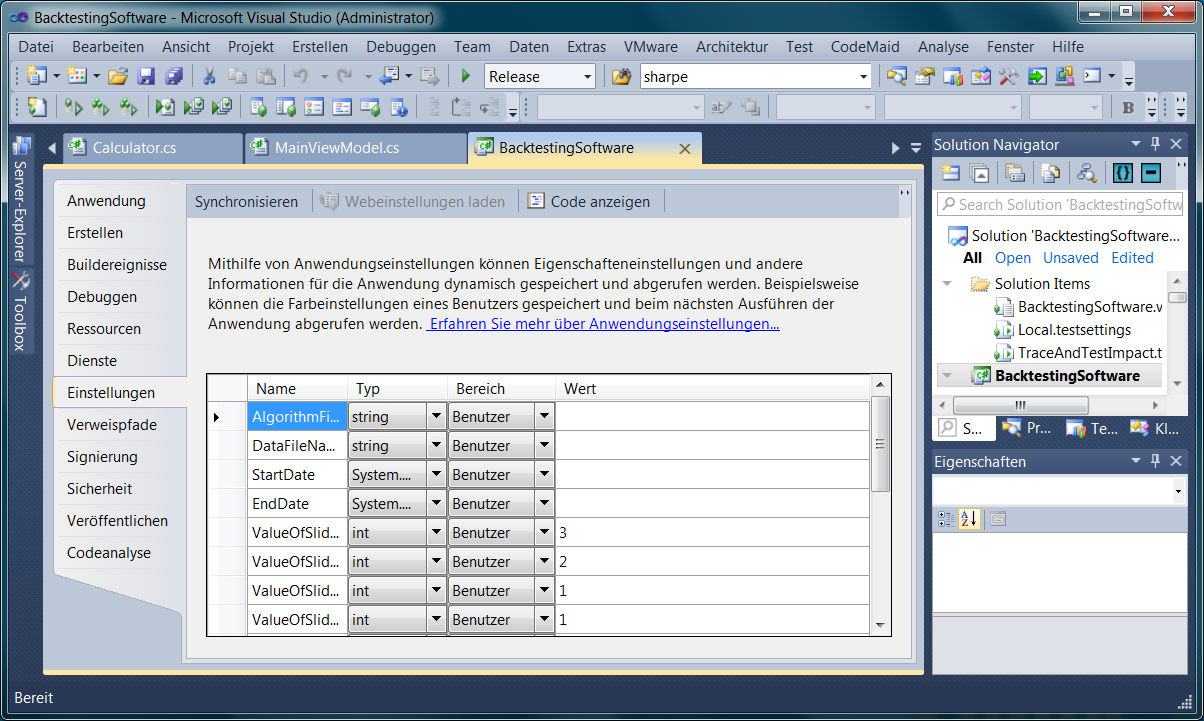
\includegraphics[width=0.90\textwidth]{graphics/grundlagen/akdErstellung.png}
	\caption{Erstellung einer Anwendungskonfigurationsdatei mit Hilfe von Microsoft Visual Studio}
	\label{fig:akdErstellung}
\end{figure}

Hier wurden schon einige Datens�tze hinzugef�gt. Wie man sehen kann, muss lediglich f�r jeden neuen Datensatz eine neue Zeile angelegt werden. Danach muss der Einstellung ein Name und ein Datentyp zugewiesen werden. Spezifische Datentypen bzw. eigens kreierte Objekte k�nnen nicht als Einstellung in der Anwendungskonfigurationsdatei definiert werden, sie k�nnen allerdings bspw. in serialisierter Form als String gespeichert werden. Nun m�ssen nur noch eine der zuvor beschriebenen Code-Sektionen als Bereich und ein Startwert, der nach der Erzeugung der \gls{xml}-Datei zu Anfang als Wert dieses Datensatzes gespeichert wird, definiert werden und schon kann der Datensatz im Programmcode benutzt werden. Das Lesen und Schreiben in ein solches File im Programmcode am Beispiel eines \textit{string}s f�r den Namen der Algorithmus-\gls{dll}-Datei funktioniert wie folgt \cite{visualcsharp}:

\begin{lstlisting}[label=Nutzung einer Anwendungskonfigurationsdatei,caption=Nutzung einer Anwendungskonfigurationsdatei]
string algorithmFileName = "algorithm.dll";
//Schreiben
Properties.Settings.Default.AlgorithmFileName = algorithmFileName;
//Lesen
string algorithmFileNameRestored = Properties.Settings.Default.AlgorithmFileName;
\end{lstlisting}

Zu den Default-Settings auf die in diesem Beispiel zugegriffen wird, k�nnen nat�rlich auch noch weitere Settings definiert werden. \cite{visualcsharp}
% LINQ
\lstset{style=sharpc}
\subsection{LINQ} \label{linq}

\gls{linq} stellt eine Spracherweiterung zu .NET dar, die mit dem .NET-Framework 3.5 und der Visual Studio Version 2008 hinzugef�hgt wurde. \gls{linq} erm�glicht es �ber ein neues Abstraktionsmodell aus vielen verschiedenen Datenquellen �ber die selbe Syntax Daten abzufragen. Unterst�tzt werden bspw. \gls{xml}-Dokumente, Datenbanktabellen, Excel-Tabellen, herk�mmliche Objekte oder Auflistungen von Objekten aller Art, und vieles mehr. \cite{visualcsharp}\\
\\
Da der Zugriff auf unterschiedliche Datenquellen intern allerdings durchaus unterschiedlich ablaufen muss, wurden von Microsoft mehrere \gls{linq}-Implementierungen in das .NET-Framework integriert. Diese werden Provider genannt und existieren zum Beispiel f�r folgende Datenquellen \cite{visualcsharp}:

\begin{itemize}
\item \textbf{\gls{linq} to Objects} \\
	Mit dieser Implementierung lassen sich Auflistungen und Objekte manipulieren, die untereinander auch in Beziehung gesetzt werden k�nnen. Sie stellt damit das Fundament aller\gls{linq}-Abfragen dar.
\item \textbf{\gls{linq} to \gls{xml}} \\
	Diese Implementierung nutzt das .NET sprachinterne Abfrage-Framework f�r den Zugriff auf \gls{xml} im Arbeitsspeicher.
\item \textbf{\gls{linq} to \gls{sql}} \\
	Hiermit kann auf Microsofts hauseigenes Datenbanksystem \gls{sql} Server 2005 und 2008 zugegriffen werden.
\end{itemize} \cite{visualcsharp}

\subsubsection{Aufbau einer LINQ-Anweisung}

Optisch sieht der Aufbau einer \gls{linq}-Anweisung, dem einer \gls{sql}-\textit{SELECT}-Anweisung sehr �hnlich. Eine Abfrage zur Ermittlung aller Personen mit Alter �ber 30 Jahren und der R�ckgabe derer Alter und Namen in einer Ergebnisliste, w�rde als \gls{linq}-Anweisung in etwa so aussehen \cite{visualcsharp}:

\begin{lstlisting}
var pers = from p in personen
		   where p.Alter > 30
		   select new { p.Name, p.Alter };
\end{lstlisting} \cite{visualcsharp}

Genau die selbe Funktion, nur mit einer anderen Formulierung w�rde auch die folgende Abfrage erf�llen \cite{visualcsharp}:

\begin{lstlisting}
var pers = personen
		  .Where( p => p.Alter > 30 )
		  .Select( p => new {p.Name, p.Alter });
\end{lstlisting} \cite{visualcsharp}

Dabei ist es v�llig egal, ob \textit{personen} das Ergebnis einer Datenbankabfrage oder eine Liste von \textit{Person}-Objekten ist, mit \gls{linq} muss man nur eine der beiden gezeigten Abfrage-Varianten benutzen.  Weiters erm�glicht die Nutzung von \gls{linq} auch viele zus�tzliche Optionen, die das Suchergebnis weiter verfeinern. Es gibt bspw. die \gls{sql}-�hnlichen Funktionen, wie \textit{GroupBy} und \textit{Join}, es gibt allerdings auch noch viele mehr. \cite{visualcsharp}

\subsubsection{Interne Funktionsweise von LINQ-Abfragen}

\gls{linq}-Abfragen machen oft Gebrauch vom Prinzip der \textit{Delegates}. \textit{Delegate} ist eine relativ alte Technologie, die in der Programmiersprache C schon unter dem Namen Funktionszeiger bekannt war. Ein \textit{Delegate} ist ein Typ, der auf eine Methode zeigt. Das Wort ''Delegate'' kommt von ''Delegierter'' und wurde gew�hlt, da ein \textit{Delegate} wirklich einen Methodenaufruf an eine bestimmte andere Methode weiter leitet. Dies wird innerhalb von \gls{linq}-Abfragen ben�tigt, um die vom User �bergebenen Bedingungen in die Logik der intern genutzten Methoden integrieren zu k�nnen. Der wohl am meisten in Kombination mit \gls{linq}-Abfragen genutzte \textit{Delegate} ist der folgende \cite{visualcsharp}:

\begin{lstlisting}
public delegate TResult Func<T, TResult>(T arg)
\end{lstlisting} \cite{visualcsharp}

Dieser wurde bspw. im oberen Beispiel verwendet, um die Bedingungen der \textit{Where}- (\textit{p => p.Alter > 30}) und der \textit{Select}-Abfrage (\textit{p => new {p.Name, p.Alter }}) an die \gls{linq}-Logik zu �bergeben. Beide dieser Bedingungen werden hier als Methodenaufrufe bzw. Zeiger auf Methodenaufrufe mit einem R�ckgabewert an die innere Logik der \gls{linq} �bergeben. Das \textit{T} in \textit{Func<T, TResult>} beschreibt einen generischen Datentypen mit dem innerhalb der Abfrage gearbeitet werden soll. Hier k�nnen alle existierenden primitiven Datentypen �bergeben werden und die Logik der \gls{linq} kann problemlos damit arbeiten. \textit{TResult} beschreibt ebenfalls einen generischen Datentypen. Allerdings den der vom angezeigten Methodenaufruf zur�ckgegeben wird. Intern ist die Abfragelogik der \gls{linq} damit so organisiert \cite{visualcsharp}:

\begin{lstlisting}
class Programm {
	static void Main(string[] args) {
		string[] arr = { "Peter", "Uwe", "Willi", "Udo" };
		GetShortNames(arr, name => name.Length < 4 );
		Console.ReadLine();
	}
	
	static void GetShortNames<T>(T[] names, Func<T, bool> getNames) {
		foreach (T name in names )
			if (getNames(name))
				Console.WriteLine(name);
	}
}
\end{lstlisting} \cite{visualcsharp}

In diesem Beispiel wird der Methode \textit{GetShortNames} ein \textit{Delegate} �bergeben, der angibt welche Namen der Namensliste ausgegeben werden soll. Hierbei h�tte in der \textit{Main}-Methode auch jede beliebige andere Bedingung, wie zum Beispiel die Abfrage, ob der erste Buchstabe des Namens ein ''P'' ist (\textit{GetShortNames(arr, name => name[0] == 'P');}) und es w�re genauso der entsprechende Name ''Peter'' ausgegeben worden, ohne dass die Methode ge�ndert werden musste. \cite{visualcsharp}


\section{F\#-Grundlagen}

% F# in Verbindung mit anderen Sprachen
% Was sind DLLs
% Pattern-Matching
% Piping-Operator
% Funktionsweise von Arrays, Lists, Sequences
% Datenstruktur-Performance (Messung, EMA)
%
% Chapter4
\chapter{Durchf�hrung} \label{chapter:durchfuehrung}

\section{Backtesting-Software}

% GUI und XAML
\lstset{style=sharpc}
\subsection{Aufbau der grafischen Benutzeroberfl�che} \label{aufbauGUI}

Als Grundelement der \gls{gui} der \gls{bts} wurde innerhalb des obligatorischen \inline{Window}s das \inline{DockPanel} gew�hlt. In diesem k�nnen weitere Elemente eingeh�ngt werden. Damit einige der inneren Elemente �ber eine Bindung ihre Daten erhalten bzw. speichern k�nnen, wurde im \inline{Window} auch noch der \inline{DataContext} auf die \inline{MainViewModel} Klasse gesetzt, in der alle \gls{gui}-relevanten Informationen gespeichert werden:

\begin{lstlisting}[label=Setzen des DataContext in XAML,caption=Setzen des DataContext in XAML]
<Window.DataContext>
	<local:MainViewModel x:Name="mainViewModel" />
</Window.DataContext>
\end{lstlisting}

\subsubsection{Men�-, Symbol-, und Sta\-tus\-leiste}

Als erstes wurde die Men�leiste (mit Hilfe des \inline{Menu}-Elements) ins \inline{Top} des \inline{Dock-} \inline{Panel}s hinzugef�gt. In dieser k�nnen \inline{MenuItem}s definiert werden. Diese stellen die einzelnen Buttons in der Men�leiste dar. Innerhalb dieser \inline{MenuItem}s k�nnen erneut \inline{MenuItem}s definiert werden. Diese beschreiben wiederum die Unterpunkte der einzelnen Buttons, die beim Dar�berhalten der Maus angezeigt werden. Auf �hnliche Art und Weise k�nnten hier auch noch weitere Ebenen erg�nzt werden. Statt der \inline{MenuItem}s k�nnen auch immer sog. \inline{Separator}s definiert werden. Diese separieren optisch Gruppen von \inline{MenuItem}s voneinander und werden als senkrechte oder waagrechte Trennlinie angezeigt. Um die \inline{MenuItem}s auch noch jeweils mit einer Aktion zu versehen, kann einfach das \inline{Click}-Feld der einzelnen Items mit einem entsprechenden Methodenkopf gef�ttert werden, der das richtige Senderobjekt und \inline{RoutedEventArgs} als Parameter �bergeben bekommt und die gew�nschte Aktion bei einem Klick beschreibt. Ein Teil des Men�s der \gls{bts} sieht demnach so aus:

\begin{lstlisting}[label=Teil der Men�leiste der BTS,caption=Teil der Men�leiste der BTS]
<Menu IsMainMenu="True" DockPanel.Dock="Top">
	<MenuItem Header="_File">
		<MenuItem Header="_Open" Click="LoadButton_Click"/>
		<Separator />
		<MenuItem Header="E_xit" Click="ExitButton_Click"/>
	</MenuItem>
	<MenuItem Header="_Help">
		<MenuItem Header="_Contact" Click="ContactButton_Click" />
		<MenuItem Header="_About" Click="AboutButton_Click" />
	</MenuItem>
</Menu>
\end{lstlisting}

Die n�chste Zeile wurde mit Hilfe der \inline{ToolBar} realisiert. In dieser k�nnen alle m�glichen Arten von \inline{Button}s und ebenfalls \inline{Separator}s angezeigt werden. Hier wurden die \inline{Button}s auch noch mit Icons versehen. Wie dies und ein Teil der \inline{ToolBar} der \gls{bts} funktionieren, kann man hier sehen:

\begin{lstlisting}[label=Teil der Toolbar der BTS,caption=Teil der Toolbar der BTS]
<ToolBar ToolBarTray.IsLocked="True" DockPanel.Dock="Top">
	<Button ToolTip="Start Performance Measurement" Click="StartButton_Click" Height="25" Width="25">
		<Image Source="images/start.ico"></Image>
	</Button>
</ToolBar>
\end{lstlisting}

Die Statusleiste unten im Fenster der \gls{bts} wurde mit der \inline{StatusBar} realisiert, die haupts�chlich den aktuellen Zustand der Anwendung anzeigt. Im \gls{xaml}-Code sieht dies wie folgt aus:

\begin{lstlisting}[label=Teil der Statusleiste der BTS,caption=Teil der Statusleiste der BTS]
<StatusBar DockPanel.Dock="Bottom">
	<StatusBarItem HorizontalContentAlignment="Stretch">
	<TextBlock Name="StatusLabel">Ready</TextBlock>
	</StatusBarItem>
	<StatusBarItem HorizontalAlignment="Right">
		<ProgressBar Height="15" Width="100" Name="ProgressBar" Visibility="Hidden" />
	</StatusBarItem>
</StatusBar>
\end{lstlisting}

Im \inline{StatusLabel} wird immer in Textform angezeigt, woran die \gls{bts} gerade arbeitet und etwaige Fehler, die w�hrend der Berechnungen aufgetreten sind. Die \inline{ProgressBar} zeigt an, wie weit die Software mit dem jeweiligen Arbeitsschritt bereits gekommen ist.\\
\\
Die Umsetzung der Leisten kann man in Abbildung \ref{fig:btsBars} erkennen.

\begin{figure}[h]
	\centering
		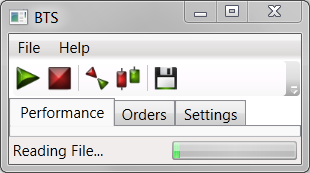
\includegraphics[width=0.50\textwidth]{graphics/durchfuehrung/btsBars.png}
	\caption{Men�-, Symbol-, und Statusleiste der fertigen BTS}
	\label{fig:btsBars}
\end{figure}

\subsubsection{TabControl}

Der eigentliche Inhalt, den die \gls{bts} haupts�chlich darstellen soll, befindet sich im gro�en mittleren Bereich, der durch ein \inline{TabControl} in drei Tabs (\inline{TabItem}s) unterteilt ist.\\
\\
Das erste Tab ist das "`Performance"'-Tab, das die allgemeinen Performance-Daten �ber den getesteten Algorithmus ausgibt. Die Oberfl�che ist hier allgemein durch ein \inline{StackPanel} und darin durch 11 Reihen aus je zwei \inline{Label}s realisiert. Das jeweils linke \inline{Label} gibt dabei an, was der Wert im rechten \inline{Label} bedeutet und das rechte \inline{Label} ist direkt mit dem entsprechenden Property aus dem \inline{MainViewModel} �ber Data Binding (siehe Abschnitt \ref{databinding} "`Data Binding"') verbunden. Das Aussehen der \gls{bts} auf dem Performance-Tab kann der Abbildung entnommen werden.\\

\begin{figure}[h]
	\centering
		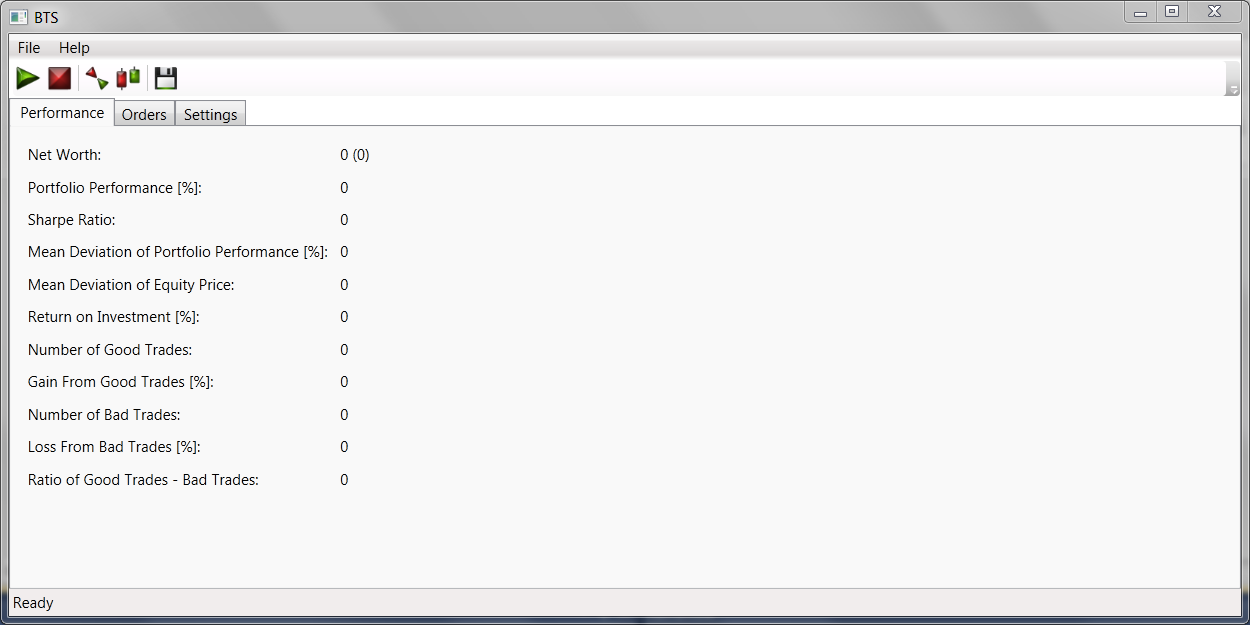
\includegraphics[width=0.90\textwidth]{graphics/durchfuehrung/btsPerformance.png}
	\caption{Performance-Tab der \gls{bts}}
	\label{fig:btsPerformance}
\end{figure}

Das zweite Tab ist das "`Orders"'-Tab, das durch ein Grid-Layout in zwei gleich gro�e Teile geteilt wird. Oben wird mittels eines \inline{WinFormsHost}s (siehe Abschnitt \ref{winformshost} "`Nutzung mit WPF"') eine Microsoft Chart Control gezeichnet, die nach dem Einlesen der Daten-Datei in der \gls{bts} das entsprechende Chart mit ggf. auch entsprechenden Indikatoren anzeigt. Im unteren Bereich wird ein \inline{DataGrid} angezeigt, das alle wichtigen Informationen �ber jede Handelsaktion ausgibt, die der Algorithmus �ber die historischen Aktien-Preisdaten get�tigt h�tte. Die Daten bekommt das \inline{DataGrid} �ber eine spezielle Art des Data Bindings, bei der der \inline{DataContext} des DataGrids im C\#-Code manuell auf die \inline{Orders}-Liste des ViewModels gesetzt wird. Die funktioniert so:

\begin{lstlisting}[label=Setzen des DataContext eines DataGrids,caption=Setzen des DataContext eines DataGrids]
this.orders.DataContext = this.mainViewModel.Orders;
\end{lstlisting}

Das \inline{DataGrid} muss daraufhin im \gls{xaml}-Code wie folgt erzeugt werden:

\begin{lstlisting}[label=Orders-DataGrid der BTS in XAML,caption=Orders-DataGrid der BTS in XAML]
<DataGrid Name="orders" Grid.Row="3" Grid.Column="0" Margin="0" ItemsSource="{Binding}"
 HorizontalAlignment="Stretch" CanUserReorderColumns="True" CanUserResizeColumns="True" IsReadOnly="True" AutoGeneratingColumn="OnAutoGeneratingColumn"/>
\end{lstlisting}

Das Aussehen dieses Tabs nach einer Beispielberechnung kann der Abbildung entnommen werden. \\

\begin{figure}[h]
	\centering
		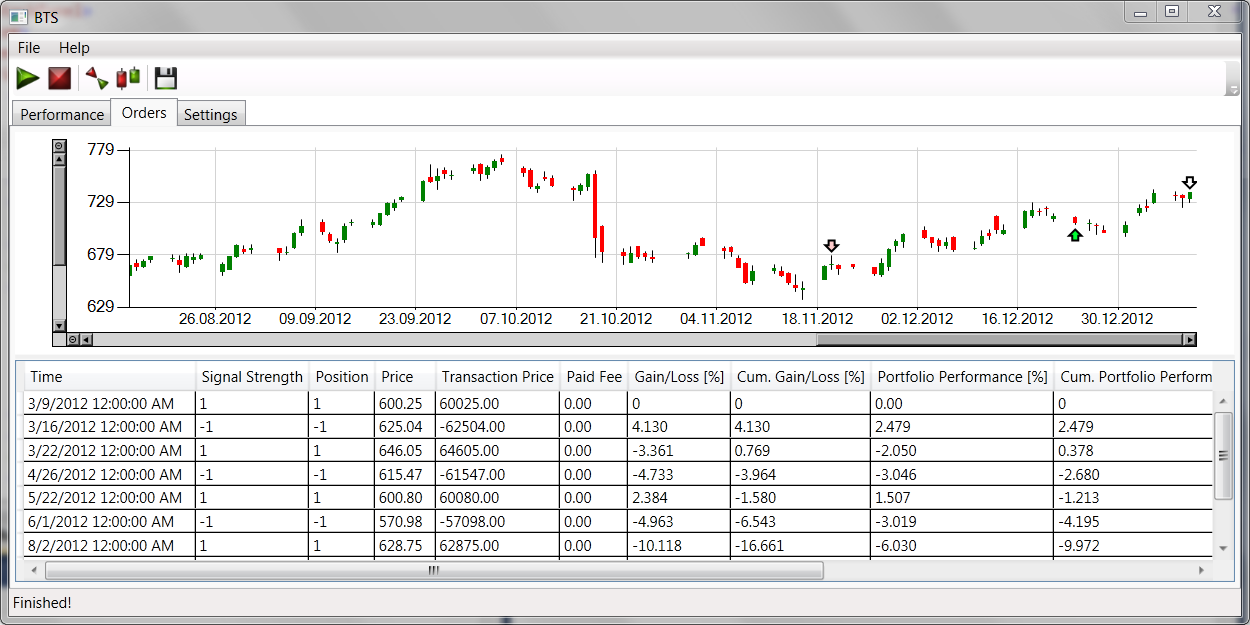
\includegraphics[width=0.90\textwidth]{graphics/durchfuehrung/btsOrders.png}
	\caption{Orders-Tab der \gls{bts} nach einer Beispielberechnung}
	\label{fig:btsOrders}
\end{figure}

Das dritte und letzte Tab ist das "`Settings"'-Tab. Auf diesem k�nnen jegliche Einstellungen, die das Laufzeitverhalten der \gls{bts} beeinflussen, getroffen werden. Dieses Tab nutzt auf der linken Seite einen \inline{TreeView} zur Auswahl der verschiedenen Seiten des Settings-Tabs. Die einzelnen Seiten auf der rechten Seite wiederum wurden durch ein weiteres \inline{TabControl} realisiert, bei dem der Kopf (in dem man normalerweise zwischen den einzelnen Tabs wechseln kann) einfach ausgeblendet wurde. Wann immer allerdings im \inline{TreeView} ein neues Item ausgew�hlt wird, wird eine besondere Methode aufgerufen, die den \inline{TabControl} auf der rechten Seite auf das richtige Tab wechseln l�sst. Dies erweckt den Anschein, dass man durch die Auswahl eines Elements im \inline{TreeView} direkt das Fenster auf der rechten Seite wechseln kann. Der \inline{TreeView} sieht im \gls{xaml}-Code wie folgt aus:

\begin{lstlisting}[label=Settings-TreeView der BTS in XAML,caption=Settings-TreeView der BTS in XAML]
<TreeView Grid.Row="0" Grid.Column="0">
	<TreeViewItem Name="GeneralSettingsTabSelector" Header="General" Selected="TreeViewItem_Selected">
	</TreeViewItem>
	<TreeViewItem Name="OrdersSettingsTabSelector" Header="Orders" Selected="TreeViewItem_Selected">
	</TreeViewItem>
	<TreeViewItem Name="ChartSettingsTabSelector" Header="Chart" Selected="TreeViewItem_Selected">
	</TreeViewItem>
</TreeView>
\end{lstlisting}

Die dazugeh�rige Methode \inline{TreeViewItem\_Selected} sieht so aus:

\begin{lstlisting}[label=Methode zum Wechseln von Tabs aus einem TreeView,caption=Methode zum Wechseln von Tabs aus einem TreeView]
private void TreeViewItem_Selected(object sender, RoutedEventArgs e)
{
	if (e.Source == this.GeneralSettingsTabSelector)
		this.GeneralSettingsTab.IsSelected = true;
	else if (e.Source == this.OrdersSettingsTabSelector)
		this.OrdersSettingsTab.IsSelected = true;
	else if (e.Source == this.ChartSettingsTabSelector)
		this.ChartSettingsTab.IsSelected = true;
}
\end{lstlisting}

Das Aussehen des Settings-Tabs auf der "`Chart"'-Seite kann der Abbildung \ref{fig:btsChartSettings} entnommen werden.

\begin{figure}[h]
	\centering
		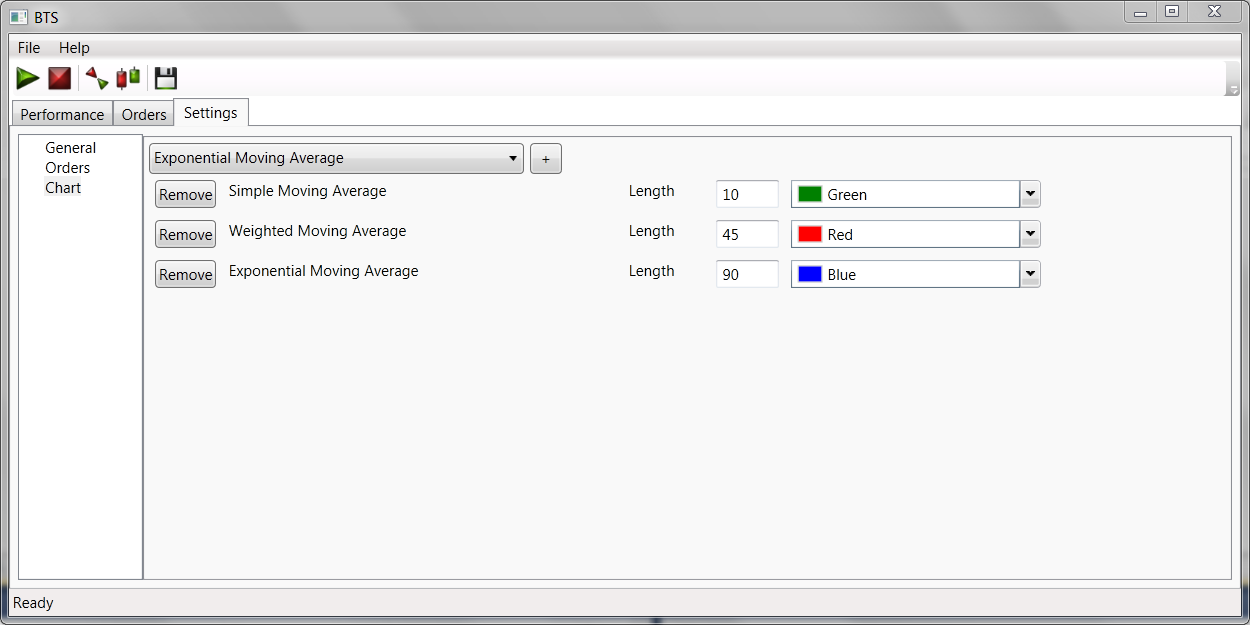
\includegraphics[width=0.90\textwidth]{graphics/durchfuehrung/btsChartSettings.png}
	\caption{Settings-Tab der \gls{bts} auf der Chart-Seite mit Beispielindikatoren}
	\label{fig:btsChartSettings}
\end{figure}

\subsubsection{Settings-Tabs}

Generell kann hier wieder zwischen drei Tabs unterschieden werden. Das erste, das "`General"'-Tab, ist recht simpel. Es bietet einfach nur die M�glichkeit, ein Algorithmus- und ein Daten-File (mit Zeitraum, in dem die Daten ausgelesen werden sollen) auszuw�hlen. Alle Komponenten daf�r sind an die entsprechenden Properties im ViewModel gebunden.\\
\\
Das zweite, das "`Orders"'-Tab, bietet alle Einstellungen bez�glich der Berechnungen der Orders innerhalb der Software. Zuerst kann ein fiktives Kapital konfiguriert werden, mit dem die \gls{bts} in ihren Berechnungen arbeitet und an dem die absoluten Zahlen f�r die Performance gemessen werden. Danach kann sowohl eine absolute als auch eine relative (in Prozent) Transaktionsgeb�hr konfiguriert werden, die dann ebenfalls in den Berechnungen der \gls{bts} von jeder Transaktion bzw. dem Gewinn oder Verlust jeder Transaktion abgezogen wird. Weiters kann ein sog. Price Premium konfiguriert werden, bei dem die \gls{bts} in weiteren Berechnungen davon ausgeht, dass die Aktien nicht immer zum normalen Handelspreis, sondern zum Handelspreis plus dem Price Premium gekauft oder dem Handelspreis minus dem Price Premium verkauft werden.  Zu guter Letzt kann noch mittels vertikaler \inline{Slider} und \inline{TextBox}en eingestellt werden, wie viele Round Lots (gr��ere Mengen von Aktien, deren Gr��e direkt darunter konfiguriert werden kann) die \gls{bts} fiktiv bei dem jeweiligen Signal des Algorithmus kaufen bzw. verkaufen soll. All diese \gls{gui}-Komponenten werden ebenfalls mit Hilfe von Data Binding mit dem ViewModel verkn�pft. Um bei den \inline{TextBox}en nur die Eingabe von Zahlen zu erm�glichen, kam auch folgende Methode �fter im Feld \inline{PreviewTextInput} der \inline{TextBox}en zum Einsatz:

\begin{lstlisting}[label=Zahleneingabefilter mit dem TextCompositionEvent,caption=Zahleneingabefilter mit dem TextCompositionEvent]
private void NumericOnly_WithDecimalPlace(System.Object sender, System.Windows.Input.TextCompositionEventArgs e)
{
	Regex reg = new Regex("[^0-9,]");
	e.Handled = reg.IsMatch(e.Text);
}
\end{lstlisting}

Das dritte, das "`Chart"'-Tab, ist das technologisch wohl spannendste der drei Tabs. Hier k�nnen einzelne Indikatoren ausgew�hlt und hinzugef�gt werden, die nach einer Berechnung automatisch in das Chart im Orders-Tab eingezeichnet werden. Wenn man einen solchen Indikator hinzuf�gt, wird intern ein neues \inline{StackPanel} mit den jeweiligen Optionen f�r den Indikator eingeblendet. Die Informationen dieser \inline{StackPanel}s werden nicht wie gew�hnlich im ViewModel gespeichert, sondern nur intern in einer Liste mit allen \inline{StackPanel}s verwaltet, aus denen direkt die Informationen der einzelnen Panels ausgelesen werden k�nnen. Jedes \inline{StackPanel} besitzt, wie man in Abbildung \ref{fig:btsChartSettings} erkennen kann, auch einen \inline{ColorPicker}, mit dem die Farbe ausgew�hlt werden kann, in der der Indikator eingezeichnet werden soll. Dieser \inline{ColorPicker} ist nicht direkt in das .NET-Framework integriert, er muss zus�tzlich aus dem Extended WPF Toolkit \cite{extended-wpf-toolkit} von Xceed bezogen werden, das die normale .NET-Library um einige \gls{wpf}-Komponenten erweitert. 
% Chartumsetzung
\subsection{Umsetzung des Charts}

Generell soll nach jeder Berechnung in der \gls{bts} zus�tzlich zur Ausgabe der berechneten Performancedaten auch ein Chart gezeichnet werden, das die �bergebenen Aktien-Preisdaten, die Entscheidungen des Algorithmus und ggf. Indikatoren f�r den Benutzer in einem Candlestick-Chart visualisiert. Der allgemeine Aufbau eines solchen Charts kann unter \ref{charting} ''Microsoft Chart Controls'' nachgelesen werden.

\subsubsection{Darstellung der Bars}

Nach dem anf�nglichen Erstellen eines \textit{Chart}s und einer \textit{Series}, muss die neue \textit{Series} zun�chst so konfiguriert werden, dass es nach einem echten Candlestick-Chart aussieht. Dies funktioniert so:

\begin{verbatim}
// Typ der Series auf Candlestick setzen
chart.Series["Data"].ChartType = SeriesChartType.Candlestick;

// Achsenbezeichnungen und Datentypen zur inneren Verwaltung definieren
chart.Series["Data"].XValueMember = "DateStamp";
chart.Series["Data"].XValueType = ChartValueType.DateTime;
chart.Series["Data"].YValueMembers = "HighPrice, LowPrice, OpenPrice, ClosePrice";

//Entsprechende Farben f�r positive und negative Bars setzen
chart.Series["Data"]["PriceUpColor"] = "Green";
chart.Series["Data"]["PriceDownColor"] = "Red";

//Zooming der Y-Achse durch den User erm�glichen und Scrollbalken definieren.
chart.ChartAreas[0].CursorY.IsUserEnabled = true;
chart.ChartAreas[0].CursorY.IsUserSelectionEnabled = true;
chart.ChartAreas[0].AxisY.ScaleView.Zoomable = true;
chart.ChartAreas[0].AxisY.ScrollBar.IsPositionedInside = false;

//Zooming der X-Achse durch den User erm�glichen und Scrollbalken definieren.
chart.ChartAreas[0].CursorX.IsUserEnabled = true;
chart.ChartAreas[0].CursorX.IsUserSelectionEnabled = true;
chart.ChartAreas[0].AxisX.ScaleView.Zoomable = true;
chart.ChartAreas[0].AxisX.ScrollBar.IsPositionedInside = false;
\end{verbatim}

Ein weiterer wichtiger Bestandteil der Darstellung ist auch noch die Skalierung und das Zooming zu Beginn. Anfangs wird auf die letzten 100 Werte gezoomt, sofern mindestens so viele vorhanden sind. Insgesamt soll das Diagramm allerdings auch nur einen ein wenig gr��eren Bereich darstellen, als Daten vorhanden sind und nicht die gesamte Skala bis hinunter zu 0. Die X-Achse wird vom Chart selbst automatisch entsprechend skaliert. Es m�ssen also zuerst der gr��te und der kleinste Wert sowohl in der gesamten Aktien-Preisdatenliste als auch in den letzten 100 Bars gesucht und gespeichert werden. Nachdem diese gefunden wurden, m�ssen 5\% aufgeschlagen werden, um das Diagramm sch�ner zu machen und entsprechend auf die gefundenen Werte f�r das gesamte Chart skaliert werden:

\begin{verbatim}
decimal margin = (max - min) * 5 / 100;
chart.ChartAreas[0].AxisY.Minimum = Math.Round(Convert.ToDouble(min - margin));
chart.ChartAreas[0].AxisY.Maximum = Math.Round(Convert.ToDouble(max + margin));
\end{verbatim}

Beim Zooming geschieht etwas sehr �hnliches, lediglich muss hier eine andere Variable der \textit{ChartArea} beeinflusst werden. F�r den Zoom der X-Achse muss das Datum 100 Bars vor dem letzten und das des letzten eingestellt werden. Dies wird allerdings aufgrund der Datentypenfreiheit dieser Angabe als double-Wert verlangt und muss deshalb mit Hilfe der Methode \textit{ToOADate()} in ein Datum im OLE Automation Format umgerechnet werden. Weiters m�ssen die Grenzen der y-Achse erneut mit einem Aufschlag von 5\% auf die zuvor gesuchten Werte definiert werden. Im Code sieht das wie folgt aus:

\begin{verbatim}
chart.ChartAreas[0].AxisX.ScaleView.Zoom(this.mainViewModel.BarList[this.mainViewModel.BarList.Count - 100].Item1.ToOADate(),
                             this.mainViewModel.BarList[this.mainViewModel.BarList.Count - 1].Item1.ToOADate());
decimal margin100 = (max100 - min100) * 5 / 100;
chart.ChartAreas[0].AxisY.ScaleView.Zoom(Math.Round(Convert.ToDouble(min100 - margin100)), Math.Round(Convert.ToDouble(max100 + margin100)));
\end{verbatim}

Nun da das Aussehen der \textit{Series} definiert ist, m�ssen nun nur noch die Daten, die vom Benutzer �bergeben wurden korrekt in diese �bernommen werden. Dazu muss die gesamte Preisliste in einer Schleife durchgegangen werden, um aus jedem Bar-Tupel den Open-, den High-, den Low- und den Close-Wert auslesen und in die \textit{Series} speichern zu k�nnen. Dies muss f�r jeden Bar-Tupel so durchgef�hrt werden, wobei auch die Reihenfolge sehr wichtig ist:

\begin{verbatim}
// Hinzufuegen des TimeStamos und des High-Werts
chart.Series["Data"].Points.AddXY(this.mainViewModel.BarList[i].Item1, Convert.ToDouble(this.mainViewModel.BarList[i].Item3));
// Hinzufuegen des Low-Werts
chart.Series["Data"].Points[i].YValues[1] = Convert.ToDouble(this.mainViewModel.BarList[i].Item4);
// Hinzufuegen des Open-Werts
chart.Series["Data"].Points[i].YValues[2] = Convert.ToDouble(this.mainViewModel.BarList[i].Item2);
// Hinzufuegen des Close-Werts
chart.Series["Data"].Points[i].YValues[3] = Convert.ToDouble(this.mainViewModel.BarList[i].Item5);
\end{verbatim}

\subsubsection{Annotations}

Im Laufe des Projekts wurde entschieden, dass die Entscheidungen des Algorithmus im Chart in Form von \textit{ArrowAnnotation}s dargestellt werden sollen. Diese sind einfache Pfeile, die an einen bestimmten Bar in der \textit{Series} angeh�ngt werden k�nnen. Farblich wurden f�r die Pfeile der Verkaufssignale -1, -2 und -3 drei unterschiedliche Rott�ne gew�hlt. Entsprechend wurden f�r die Kaufsignale 1, 2 und 3 drei unterschiedliche Gr�nt�ne gew�hlt. Au�erdem zeigen die roten Pfeile nach unten und die gr�nen nach oben. Neutralpfeile, die das Signal 0 darstellen, sind die wei�er Farbe gehalten. Da es sich bei Neutralpfeile immer um eine Neutralisierung der zuvor eingegangenen Position sind, zeigen die Neutralpfeile bei der Neutralisierung einer Short-Position (-1, -2 oder -3) nach oben, da gekauft werden muss und bei der Neutralisierung einer Long-Position (1, 2 oder 3) nach unten, da verkauft werden muss. Die \textit{Annotation}s werden zu einer eigenen Eigenschaft des Charts, n�mlich \textit{Annotations} hinzugef�gt und die Berechnung des Aussehens der einzelnen Pfeile erfolgt direkt beim Hinzuf�gen jedes einzelnen Bars, sofern an diesem ein Signalwechsel des Algorithmus vorliegt. Die Berechnung der Signale muss daher klarerweise vor dem Aufbau des Charts erfolgen. Im Code sind \textit{ArrowAnnotation}s f�r einen roten Pfeil wie folgt realisiert. F�r die anderen Pfeile m�ssen nur die jeweiligen Eigenschaften ge�ndert werden:

\begin{verbatim}
//Erzeugen der ArrowAnnotation
ArrowAnnotation a = new ArrowAnnotation();
//Vergabe eines Namens, da nicht alle gleich heissen duerfen
a.Name = "Arrow-" + i;
//Anhaengen an die ChartArea
a.ClipToChartArea = chart.ChartAreas[0].Name;

//Hoehe des Pfeils, -5 da er nach unten zeigen soll.
//Mit 5 waere er gleich gross, wuerde aber nach oben zeigen
a.Height = -5;
//Aussenlinien werden schwarz gefaerbt
a.LineColor = System.Drawing.Color.Black;
//Im inneren wird der entsprechende Rotton fuer das jeweilige Signal ausgewaehlt.
switch (this.mainViewModel.Signals[i])
{
    case -1:
        a.BackColor = System.Drawing.Color.FromArgb(255, 204, 204);
        break;
    case -2:
        a.BackColor = System.Drawing.Color.FromArgb(255, 0, 0);
        break;
    case -3:
        a.BackColor = System.Drawing.Color.FromArgb(102, 0, 0);
        break;
}

//Gibt an, an welchem Bar in der Series der Pfeil befestigt werden soll
a.AnchorDataPoint = chart.Series["Data"].Points[i];
//Gibt an, dass der high-Wert als Ausgang fuer den Pfeil gewaehlt werden soll
a.AnchorY = chart.Series["Data"].Points[i].YValues[0];
//Gibt an das der Pfeil vom Anker noch ein wenig nach oben verschoben werden soll
a.AnchorOffsetY = -2;

//Hinzufuegen zum Chart
chart.Annotations.Add(a);
\end{verbatim}

\subsubsection{Indikatoren}

Grunds�tzlich k�nnen in der \gls{bts} auf dem Settings-Tab unter ''Chart'' neue Indikatoren hinzugef�gt werden, die bei der Erstellung des Charts nach einer Berechnung automatisch in neue \textit{Series} eingezeichnet und so dargestellt werden sollen. Intern wird dazu in der \gls{bts} eine Liste aus \textit{StackPanel}s gespeichert. Wenn ein neuer Indikator hinzugef�gt wird, wird in dieser Liste ein neues \textit{StackPanel} erzeugt. Dieses beinhaltet, je nach Indikator den es repr�sentieren soll, unterschiedliche \gls{wpf}-\gls{gui}-Komponenten, die alle notwendigen Informationen speichern k�nnen. Es wurde die Unterst�tzung vier verschiedener Indikatoren (f�r finanzwirtschaftliche Erkl�rung siehe Abschnitt \ref{Indikatoren} ''Indikatoren'') implementiert:

\begin{itemize}
\item \textbf{Simple Moving Average} \\
	Der \gls{sma} speichert seinen Namen, eine L�nge, �ber die er berechnet werden soll und eine Farbe, in der er gezeichnet werden soll.
\item \textbf{(Linear) Weighted Moving Average} \\
	Der \gls{lwma} speichert die gleichen Werte wie der \gls{sma}, er unterscheidet sich nur in der Berechnung.
\item \textbf{Exponential Moving Average} \\
	Auch der \gls{ema} speichert die gleichen Werte wie der \gls{sma} und unterscheidet sich nur in der Berechnung.
\item \textbf{Moving Average Convergence/Divergence} \\
	Der \gls{macd} berechnet intern zwei \glspl{ma} und ben�tigt daher die Konfiguration von zwei unterschiedlichen L�ngen. Zudem speichert aber auch er seinen Namen und die Farbe, in der er gezeichnet werden soll.
\end{itemize}

Wurden diese Indikatoren festgelegt, wird bei folgenden Berechnungen nach der einfachen bisherigen Charterstellung auch noch die bereits erw�hnte \textit{StackPanel}-Liste durchsucht. Dabei werden die Informationen jedes Indikators anhand seines Namens ausgelesen, es wird eine neue \textit{Series} erstellt und der Berechnung mittels \textit{FinancialFormula} �bergeben. Dies funktioniert wie in \ref{finfor} ''Finanzielle Berechnungen'' beschrieben und die Werte des Indikators werden dabei automatisch in die \textit{Series} geschrieben und diese kann problemlos gezeichnet werden.\\
\\
Beim zuletzt erw�hnten, dem \gls{macd} gilt es allerdings noch eine weitere Problematik zu beachten. Als einziger der implementierten Indikatoren fluktuiert der \gls{macd} n�mlich nicht um die Aktien-Preisdaten herum, sondern um die X-Achse. Da dies in der selben Zeichnung nicht wirklich sch�n aussehen w�rde, wird zur Darstellung des \gls{macd} nun eine extra \textit{ChartArea} erzeugt, die sich unter der Haupt-Area befindet. Eine solche zweite \textit{ChartArea} l�sst sich grunds�tzlich auch recht einfach auf die selbe Art und Weise wie die erste erzeugen, nur dass sie noch auf die erste \textit{ChartArea} ausgerichtet werden muss. Hier wurde eine Gr��e von 70\% des gesamten Charts f�r die Candlestick-Area und 30\% f�r die \gls{macd}-Area festgelegt. Dies funktioniert wie folgt:

\begin{verbatim}
public void drawSecondChartArea(Chart chart)
{
	//Erzeugen und hinzuf�gen der zweiten ChartArea
    ChartArea indicatorArea = new ChartArea("IndicatorArea");
    chart.ChartAreas.Add(indicatorArea);
    
    ...            
    
    //Verkn�pfung mit der Haupt-Area herstellen
    chart.ChartAreas[1].AlignWithChartArea = "MainArea";
    
    ...
    
    //Gr��e der Haupt-Area auf 70% setzen
    chart.ChartAreas[0].Position.Width = 100;
    chart.ChartAreas[0].Position.X = 0;
    chart.ChartAreas[0].Position.Height = 70;
    chart.ChartAreas[0].Position.Y = 0;

	//Gr��e der MACD-Area auf 30% setzen
    chart.ChartAreas[1].Position.Width = 100;
    chart.ChartAreas[1].Position.X = 0;
    chart.ChartAreas[1].Position.Height = 30;
    chart.ChartAreas[1].Position.Y = 70;
    
\end{verbatim}
% Algorithmus- und Dateneinbindung
\lstset{style=sharpc}
\subsection{Einbindung des Algorithmus}

Da die \gls{bts} nat�rlich nicht nur einen Algorithmus testen k�nnen soll, ist es wichtig, dass die Algorithmen nicht direkt im Code verankert sind, sondern zur Laufzeit geladen werden k�nnen. Dazu kann der Benutzer einen Pfad angeben, von dem der Algorithmus in Form einer \gls{dll}-Datei (siehe \ref{dll} "`Dynamic Link Library"') gelesen werden kann. Damit die \gls{bts} den Algorithmus aber auch ausf�hren kann, muss dieser zuerst in die lokale Dom�ne des Benutzers bzw. der \gls{bts} geladen werden. \\
Dazu gibt es zwei M�glichkeiten:

\begin{itemize}
\item \textbf{\inline{LoadFrom}} \\
	Die \inline{LoadFrom}-Methode erm�glicht es, eine Assembly (bspw. unser \gls{dll}-File) in die lokale Dom�ne zu laden und Methoden dieser Assembly aufzurufen. Ein kleines Problem hierbei ist allerdings, dass man die geladene Assembly in der Dom�ne nur sehr aufwendig �berschreiben oder l�schen kann, daher ist sie f�r unsere Anwendung nicht perfekt geeignet.
\item \textbf{\inline{LoadFile}} \\
	Die \inline{LoadFile}-Methode erf�llt nahezu den gleichen Zweck, wie die \inline{Load-} \inline{From}-Methode, nur dass man hier einfach eine zweite Assembly in die Dom�ne laden kann und die erste wird �berschrieben. Daher wird in der \gls{bts} diese Methode genutzt.
\end{itemize}

Der komplette Codeausschnitt zum Laden eines Algorithmus sieht nun wie folgt aus:

\begin{lstlisting}[label=Einbindung und Nutzung einer DLL,caption=Einbindung und Nutzung einer DLL]
//Laden des Assemblys
Assembly assembly = Assembly.LoadFile(this.mainViewModel.AlgorithmFileName);
//Laden des Assemblys in die Dom�ne
AppDomain.CurrentDomain.Load(assembly.GetName());
//Speichern der Klasse, zum spaeteren Ausfuehren von Methoden
Type t = assembly.GetType("Algorithm.DecisionCalculator");

//Uebergabeparameter der Methode, die aufgerufen wird,
//muessen als Objektarray uebergeben werden
Object[] oa = { this.mainViewModel.BarList, this.mainViewModel.Signals };
//Invokieren der Methoden mit den Uebergabeparametern
t.GetMethod("startCalculation").Invoke(null, oa);
\end{lstlisting}

Durch Aufruf der \inline{startCalculation}-Methode des Algorithmus werden die Signale in die �bergebene Liste aus dem ViewModel gespeichert. Diese k�nnen von dort anschlie�end f�r die Berechnungen benutzt werden. Hierzu ist noch wichtig zu erw�hnen, dass von der \gls{bts} an den letzten Bar noch ein Signal mit dem Wert 0 gesetzt wird, damit sp�ter in den Berechnungen alle noch offenen Positionen aufgel�st werden und man die fiktive letztendliche Performance betrachten kann, die in diesem Fall aufgetreten w�re.

\subsection{Auslesen der Aktien-Preisdaten}

Die Aktien-Preisdaten werden in Form von Bars �ber einen bestimmten Zeitraum erwartet. Ob es sich hierbei um Minute-, Daily- oder andere Bars handelt, ist hierbei grunds�tzlich egal. Sie m�ssen lediglich in Form einer \gls{csv}-Datei mit folgendem Format gespeichert werden:

\begin{lstlisting}[label=Format des CSV-Daten-Files,caption=Format des CSV-Daten-Files]
Bar,Date,Time,Open,High,Low,Close
1,01/02/90,00:00,8.8125,9.375, 8.75,9.3125
2,01/03/90,00:00,9.375, 9.50,9.375,9.375
3,01/04/90,00:00,9.375,9.6875,9.3125,9.40625
...
\end{lstlisting}

Das Datum muss im Format MM/DD/YY und die Uhrzeit im Format hh:mm gespeichert werden. Die Dezimalstellen von Open, High, Low und Close m�ssen durch einen Punkt und ohne Tausendertrennzeichen angegeben werden. Es k�nnen nat�rlich nahezu unendlich viele Bars in der Datei gespeichert werden, die Berechnungen dauern dadurch einfach entsprechend l�nger. Weiters wird die erste Zeile nicht ber�cksichtigt, da hier meist Header-Informationen gespeichert sind. Befindet sich hier auch schon ein Bar, wird dieser ignoriert. Noch genauere Informationen hierzu k�nnen dem Benutzerhandbuch (siehe Anhang \ref{appendix_A} "`Benutzerhandbuch"') von Noctua entnommen werden\\
\\
Ist der Pfad in der \gls{bts} richtig gew�hlt und die Berechnung wird gestartet, wird das \gls{csv}-File in der \gls{bts} ausgelesen. Dies geschieht mit Hilfe der \gls{linq}-Technologie (siehe \ref{linq} "`LINQ"') und sieht im Code wie folgt aus:

\begin{lstlisting}[label=LINQ zum Auslesen des CSV-Daten-Files,caption=LINQ zum Auslesen des CSV-Daten-Files]
public static IEnumerable<
	Tuple<DateTime, decimal, decimal, decimal, decimal>>
	EnumerateExcelFile(
	string filePath, DateTime startDate, DateTime endDate)
{
	// Geht alle Zeilen durch und ueberspringt den Header
	return from line in File.ReadLines(filePath).Skip(1)
		select line.Split(',')
			into fields
			//Parst die das Datum und die Uhrezit und
			//speichert es in den Tupel
			let timeStamp = DateTime.ParseExact(
				fields[1] + " " + fields[2],
				"MM/dd/yy HH:mm",
				new CultureInfo("en-US"))
			//Speichert alle anderen Werte in den Tupel
			//und beruecksichtigt Dezimalzahlen 
			let open = decimal.Parse(fields[3],
				CultureInfo.InvariantCulture)
			let high = decimal.Parse(fields[4],
				CultureInfo.InvariantCulture)
			let low = decimal.Parse(fields[5],
				CultureInfo.InvariantCulture)
			let close = decimal.Parse(fields[6],
				CultureInfo.InvariantCulture)
			//Liest nur die Bars im gew�hlten Bereich aus
			where timeStamp.Date >= startDate.Date &&
				timeStamp.Date <= endDate.Date
			//Erzeugt den Tupel und speichert ihn in das
			//Rueckgabe-IEnumerable
			select new Tuple<
				DateTime, decimal, decimal, decimal, decimal>
				(timeStamp, open, high, low, close);
}
\end{lstlisting}
% Berechnung der einzelnen Werte der Orders
% Berechnung der Performancedaten
\subsection{Berechnung der Performancedaten}

In der \gls{bts} finden sich zwei verschiedene Arten von Performancedaten. Da w�ren zum einen die Order-spezifischen, die Daten zu jeder fiktiven Kaufentscheidung in der Vergangenheit generieren und die allgemeinen, die die Performance des Algorithmus �ber den gesamten Zeitraum der Daten widerspiegeln. Wie die einzelnen Daten der beiden Kategorien berechnet werden, soll im Folgenden erl�utert werden.

\subsubsection{Order-spezifische Performancedaten}

Die Order-spezifischen Performancedaten kann man sich auf dem Orders-Tab der \gls{bts} f�r jede Order ansehen. Sie werden wie folgt berechnet:

\begin{itemize}
\item \textbf{Time} \\
	Time gibt den fiktiven Zeitpunkt in der Vergangenheit an, zu dem diese Order unter Echtzeiteinsatz des Algorithmus ausgef�hrt worden w�re.
\item \textbf{Signal Strength} \\
	Gibt die St�rke des Signals (-3 bis +3) aus, das der Algorithmus bei dieser Order gegeben h�tte.
\item \textbf{Position} \\
	Position (Pos) beschreibt die Anzahl an Round Lots die durch die Einstellungen in der \gls{bts} bei der vorliegenden Signal Strength gehandelt werden.
\item \textbf{Price} \\
	Gibt den Preis (P) an zu dem die Order zum gegebenen Zeitpunkt platziert worden w�re. Es handelt sich hierbei um den historischen Close-Wert des entsprechenden Bars. Handelt es sich um eine Kaufentscheidung wird hierzu noch der PricePremiumPercentage addiert, handelt es sich um eine Verkaufsentscheidung wird er subtrahiert.
\item \textbf{Transaction Price} \\
	Der Transaktionspreis (TP) gibt an, wie viel Kapital nun investiert werden muss, um die gegebene Anzahl an Round Lots zum gegebenen Preis (Price) handeln zu k�nnen. Die Round Lots die gekauft werden m�ssen (RLA) sind die Differenz von der alten zur neuen Position. War die alte Position also bspw. -1 und das neue ist 1, dann m�ssen zwei Round Lots gekauft werden. Hierzu werden auch alle zu zahlenden Geb�hren addiert. In der folgenden Gleichung ist RLS die Gr��e eines Round Lots.
	\begin{equation}
		\label{Transaction Price}
		TP = (P * RLS * RLA) + PF
	\end{equation}
\item \textbf{Paid Fee} \\
	Paid Fee (PF) ist die Gesamtheit aus allen relativen (RT) und absoluten (AT) Transaktionsgeb�hren, die in der \gls{bts} eingestellt wurden f�r diese Order bezahlt h�tten werden m�ssen. Dabei wird klarerweise mit dem TP vor Addition der Geb�hren gerechnet (TP0).
	\begin{equation}
		\label{Paid Fee}
		PF = (\frac{RT}{100} * TP0) + AT
	\end{equation}
\item \textbf{Gain/Loss [\%]} \\
	GainLoss (GL) beschreibt die prozentuelle Kapitalver�nderung durch vorherige Trades bis zum jetzigen relativ auf das eingesetzte Investitionskapital, also TP. Dabei wird kein unrealisierter Profit/Verlust angeschrieben, sondern nur der wirklich realisierte. Das bedeutet, dass bei einer Verst�rkung der Position der aktuellen Order im Vergleich zur letzten das GL der letzten Order nur um den entsprechende Anteil an Geb�hren, die zu zahlen sind, negativ ist. Der Anteil an den Gesamtgeb�hren (PF), der hier eingesetzt wird, kann wie folgt berechnet werden:
	\begin{equation}
		\label{Gebuehren fuer GL}
		GL0 = \frac{-PF}{TP0} * 100
	\end{equation}
	Wenn es sich daher um die Verst�rkung einer Position oder die erste Order (hier gibt es keinen Preis der letzten Transaktion oldP) handelt, kann nur GL0 angeschrieben werden. Weiters muss man bei einer Verst�rkung der Position auch noch den Preis zu dieser Zeit multipliziert mit der Quantit�t um die verst�rkt wurde  zwischengespeichert werden. Die Quantit�t, um die verst�rkt wurde (diffPos) ist lediglich die absolute Differenz zwischen dem alten und dem neuen Signal. Das Ganze wird in einer Zwischenvariable namens Ausgabe (A) gespeichert, um sp�ter noch wissen zu k�nnen wie viel f�r die gerade verf�gbaren Positionen gezahlt wurde.
	\begin{equation}
		\label{Ausgabe bei Verst�rkung der Position}
		A = A + (P * |diffPos|)
	\end{equation}
	Wird nun allerdings wirklich Positionen realisiert werden, muss der gesamte realisierte Gewinn relativ zum investierten Kapital hier angegeben werden. Hierbei sind erneut zwei F�lle m�glich. \\
	\\
	Zum einen k�nnte es sein, dass nicht alle Positionen abgebaut werden, die Vorzeichen der alten und der neuen Position also gleich sind. Daf�r muss zuerst herausgefunden werden, wie viel f�r die Positionen, die man besitzt bezahlt wurde. Dies kann nur angen�hert werden, indem man den Anteil an A ausrechnet, der gerade realisiert wird:
	\begin{equation}
		\label{Berechnung des realisierten Anteils an der Ausgabe}
		relA = \frac{A}{oldPos} * |diffPos|
	\end{equation}
	Mit diesem kann man durch Vergleich des Gewinns (aktueller Preis multipliziert mit der Anzahl an realisierten Positionen minus dem entsprechenden Anteil an der Gesamtausgabe relA) mit dem Anteil an der Ausgabe relA herausfinden, um wie viel Prozent sich das investierte Kapital durch die Realisierung der Positionen ver�ndert hat. Weiters muss vom Preisanstieg bzw. -abstieg, der �ber die Periode angefallen ist, noch der zuvor berechnete entsprechende Anteil an Geb�hren (GL0) abgezogen werden:
	\begin{equation}
		\label{Gain/Loss}
		GL = (\frac{((|diffPos| * P) - relA)}{relA}) * 100) - GL0
	\end{equation}
	Nach dieser Berechnung muss nat�rlich noch der realisierte Anteil an den Ausgaben relA von den Gesamtausgaben A abgezogen werden.\\
	\\
	Zum anderen kann es passieren, dass alle realisierten Positionen abgebaut, aber im selben Schritt m�glicherweise auch gleich wieder neue Positionen aufgebaut werden. In diesem Fall muss der Gewinn (hier Multiplikation des aktuellen Preises P mit der absoluten alten Position oldPos minus der gesamten bisherigen Ausgabe A) mit der gesamten Ausgabe A verglichen werden. Danach m�ssen nat�rlich auch hier noch die angefallenen Geb�hren abgezogen werden.
	\begin{equation}
		\label{Gain/Loss}
		GL = (\frac{((|oldPos| * P) - A)}{A}) * 100) - GL0
	\end{equation}
	Falls hier auch noch eine neue Position angelegt wurde, muss diese nat�rlich auch in den Ausgaben A vermerkt werden. Da hierdurch jedoch wieder kein realisierter Gewinn erzeugt wird, muss hier wirklich nur die Ausgabe auf 0 gesetzt (da vorher alle Positionen realisiert wurden) und die absolute neu angelegte Position vermerkt werden.
	\begin{equation}
		\label{Ausgabe beim Neuanlegen von Positionen}
		A = P * |Pos|
	\end{equation}
\item \textbf{Cumulative Gain/Loss [\%]} \\
	Hierbei werden kumulativ die GL-Werte aller bisherigen Orders aufaddiert ausgegeben.
\item \textbf{Portfolio Performance [\%]} \\
	Die Portfolio Performance (PP) ist eine der wichtigsten Performancedaten. Sie gibt an, um wie viel Prozent sich das gesamte Kapital bei dieser einen Order im Vergleich zur vorherigen ver�ndert hat, also wie gro� die Auswirkung dieses Trades auf das Kapital ist. Hierzu wird als Grundlage einfach das aktuelle Verm�gen (vgl.''Net Worth'' (NW) weiter unten) und die absolute Kapitalver�nderung (vgl. ''Absolute Portfolio Performance'' (APP) weiter unten) genommen:
	\begin{equation}
		\label{Portfolio Performance}
		PP = \frac{APP}{NW} * 100
	\end{equation}
\item \textbf{Cumulative Portfolio Performance [\%]} \\
	Hierbei werden einfach kumulativ die vorherigen Prozentwerte der Kapitalver�nderung aufaddiert. Es wird hier allerdings nicht mit der PP gearbeitet, sondern statt dem Net Worth durch das Startkapital (K) dividiert, um die gesamte Performance in Bezug auf das Gesamtkapital zeigen zu k�nnen. Die Formel zu Berechnung der einzelnen Werte sieht hier daher so aus:
	\begin{equation}
		\label{Cumulative Portfolio Performance}
		cPP = \frac{APP}{K} * 100
	\end{equation}
\item \textbf{Absolute Portfolio Performance} \\
	Dieser Wert hat grunds�tzlich die gleiche Aussage, wie die PP, nur dass er absolut angegeben wird und als Grundlage der Berechnung der PP dient. Er �hnelt in der Berechnung sehr dem GL, nur dass hier bei jeder Order auch der unrealisierte Gewinn/Verlust ausgegeben wird. Der unrealisierte Gewinn/Verlust ist die Kapitalver�nderung, die das Portfolio erfahren w�rde, wenn man alle Aktien zum aktuellen Preis verkaufen w�rde. Daher wird beim APP jede Order intern so berechnet, wie wenn man alle vorherigen Positionen verkaufen und sich die aktuellen Positionen alle neu kaufen w�rde. Die Geb�hren werden hierf�r allerdings nicht abgezogen, da dieser Handel ja nicht wirklich durchgef�hrt wird, er dient nur zur Veranschaulichung der Performance des letzten Trades. \\
	\\
	Zur Berechnung m�ssen jegliche fiktive Ver�nderungen des Kapitals durch den Ankauf bzw. Verkauf von Aktien in der vorherigen Order mitberechnet werden. Das hei�t, dass die Preis�nderungen unabh�ngig von der aktuellen Position immer nur f�r alle alten Positionen evaluiert werden m�ssen. Dies erweckt den Anschein, dass alle vorherigen Positionen neutralisiert werden, deren fiktiver Gewinn angegeben wird und sie dann quasi wieder neu aufgebaut werden. Dies funktioniert in allen F�llen, da nur die alte Position bzw. deren Performance bis zur aktuellen Order ber�cksichtigt wird. Weiters muss mit der gew�hlten Gr��e eines Round Lots (RLS) multipliziert werden, da es sich ja um absolute Werte handelt und ausschlie�lich in Round Lots gehandelt wird. Die Berechnung der APP funktioniert wie folgt:
	\begin{equation}
		\label{Berechnung der Absolute Portfolio Performance}
		APP = (P - oldP) * oldPos * RLS
	\end{equation}
\item \textbf{Cumulative Absolute Portfolio Performance} \\
	Hierbei werden kumulativ die APP-Werte aller bisherigen Orders aufaddiert ausgegeben.
\item \textbf{Net Worth} \\
	Der Net Worth zu jeder Order gibt an, wie viel Verm�gen man zum entsprechenden Zeitpunkt insgesamt h�tte, wenn man alle noch offenen Positionen zum aktuellen Preis neutralisieren w�rde. Den Ausgangswert hierf�r bietet das Startkapital.
\end{itemize}

\subsubsection{Allgemeine Performancedaten}

Zus�tzlich zu den spezifischen Performancedaten f�r jede Order auf dem Orders-Tab, k�nnen in der \gls{bts} auf dem Performance-Tab allgemeine Performancedaten gefunden werden. Diese beschreiben, wie gut der Algorithmus �ber die gesamte ausgew�hlte Periode der Aktien-Preisdaten abgeschnitten h�tte, wenn er unter normalen Bedingungen auf der B�rse gehandelt h�tte. Hier gibt es folgende Daten:

\begin{itemize}
\item \textbf{Net Worth} \\
	Hier ist der Net Worth das gesamte Kapital, dass sich dem Einsatz des Algorithmus �ber die gesamte gew�hlte Periode besessen h�tte. Es berechnet sich aus den Gewinnen und Verlusten aus allen Trades und dem Startkapital. Der Net Worth ist daher au�erdem gleich mit Order-spezifischen Net Worth nach der letzten Order.
\item \textbf{Portfolio Performance [\%]} \\
	Die allgemeine Portfolio Performance (GPP) beschreibt den gesamten prozentuellen Gewinn bzw. Verlust den der Algorithmus unter normalem Einsatz �ber die gesamte gew�hlte Periode der Aktien-Preisdaten gemacht h�tte. Er berechnet sich aus den prozentuellen Einzelgewinnen/-verlusten aller Orders relativ zum Startkapital und ist damit gleich der Order-spezifischen kumulativen Portfolio Performance nach dem letzten Trade.
\item \textbf{Sharpe Ratio} \\
	Der Sharpe Ratio ist quasi ein Wirkungsgrad der angibt, wie viele Gewinne bzw. Verluste der Algorithmus �ber die gew�hlte Periode machen konnte relativ zum dabei eingegangenen Risiko, als der Volatilit�t. Zur Beschreibung der Volatilit�t wurde in der Berechnung die Standardabweichung der Portfolio Performance (vgl. ''Mean Deviation of Portfolio Performance [\%]'' (MDPP) weiter unten). Au�erdem muss hier von den Gewinnen noch der Prozentsatz abgezogen werden, den man bei einer risikofreien Investition des gleichen Kapitals erreichen h�tte k�nnen (RF), um die eigentliche Qualit�t des Algorithmus widerspiegeln zu k�nnen. Die allgemeine Formel zur Berechnung des Sharpe Ratio lautet daher:
	\begin{equation}
		\label{Sharpe Ratio}
		SR = \frac{GPP - RF}{MDPP}
	\end{equation}
	Der Standardzinssatz (p) bei einer risikofreien Anlagen bewegt sich hierbei meist um 1.5\% pro Jahr. Daher muss hier um an RF zu kommen eine Zinseszins-Rechnung der gew�hlten Anzahl an Jahren (n), �ber die der Algorithmus rechnet, durchgef�hrt werden. Das Kapital das man durch risikofreie Anlagen aus dem Startkapital erh�lten h�tte l�sst sich daher wie folgt berechnen:
	\begin{equation}
		\label{Zinseszins-Berechnung}
		NWRF = K * (1 + \frac{p}{100})^n
	\end{equation}
	Um nun herauszufinden wie hoch dieser Prozentsatz gewesen w�re muss nun folgende Berechnung durchgef�hrt werden:
	\begin{equation}
		\label{Risikofreie Portfolio Performance}
		RF = \frac{NWRF - K}{K} * 100
	\end{equation}
\item \textbf{Mean Deviation of Portfolio Performance [\%]} \\
	Die Mean Deviation of Portfolio Performance ist die Standardabweichung der Order-spezifischen Portfolio Performance aller Orders. Generell wird die Standardabweichung wie folgt berechnet:
	\begin{equation}
		\label{Standardabweichung}
		s = \sqrt{\frac{1}{N-1} \sum_{i=1}^N (x_i-\overline{x})^2}
	\end{equation}
\item \textbf{Mean Deviation of Equity Price} \\
	Die Mean Deviation of Equity Price ist die Standardabweichung aller Close-Werte der Aktien-Preisbars in der gew�hlten Periode. Diese soll dem Nutzer einen �berblick �ber die allgemeine Volatilit�t der �bergebenen Daten verschaffen. Die Standardabweichung wird auch hier mit der allgemeinen Formel berechnet, die bspw. in der Gleichung \ref{Standardabweichung} nachgelesen werden kann.
\item \textbf{Return on Investment [\%]} \\
	Return on Investment (ROI) beschreibt die prozentuelle Kapitalver�nderung, �hnlich wie die Portfolio Performance, nur dass hier das wirklich investierte Kapital jedes Trades als Basis der Prozentrechnung herangezogen wird. Bei der Portfolio Performance ist dies n�mlich das insgesamt verf�gbare Kapital. Dieser Wert ist gleich dem Order-spezifischen kumulativen Gain/Loss nach der letzten Order.
\item \textbf{Number of Good Trades} \\
	Die Number of Good Trades (NoGT) gibt die Anzahl an Handlungen an, durch die der Algorithmus im echten Betrieb einen Gewinn erzielt h�tte. Die Klassifizierung eines Trades als Good Trade passiert allerdings bevor die entsprechend zu zahlenden Geb�hren hier mitgerechnet werden, da sonst ein Trade ohne Neutralisierung alter Positionen, bei denen nur Geb�hren gezahlt werden m�ssen automatisch als Bad Trade klassifiziert werden w�rden.
\item \textbf{Gain From Good Trades [\%]} \\
	Der Gain From Good Trades gibt an, wie viel Gewinn durch alle Good Trades zusammen gemacht h�tte werden k�nnen, g�be es keine Bad Trades. Als Grundlage dieser Berechnung wird die Portfolio Performance jedes Good Trades relativ zum Startkapital herangezogen. Es wird hier also bei jedem Good Trade der Wert addiert, der auch zur Order-spezifischen kumulativen Portfolio Performance bei jedem Trade addiert wird.
\item \textbf{Number of Bad Trades} \\
	Die Number of Bad Trades (NoBT) gibt die Anzahl an Handlungen an, durch die der Algorithmus im echten Betrieb einen Verlust erzielt h�tte. (vgl. ''Number of Good Trades'' weiter oben bez�glich der Berechnung)
\item \textbf{Loss From Bad Trades [\%]} \\
	Der Loss From Bad Trades gibt an, wie viel Verlust durch alle Bad Trades zusammen gemacht worden w�re, g�be es keine Good Trades. (vgl. ''Gain From Good Trades'' weiter oben bez�glich der Berechnung)
\item \textbf{Ratio of Good Trades - Bad Trades} \\
	Der Ratio zwischen Good und Bad Trades beschreibt deren mengenm��iges Verh�ltnis an. Dabei wird die Anzahl an Good Trades durch die Anzahl an Bad Trades dividiert. Dadurch entsteht quasi ein Wirkungsgrad bei dem Ergebnisse gr��er als 1 darauf hindeuten, dass mehr Good Trades als Bad Trades vom Algorithmus berechnet wurden. Die Berechnung funktioniert wie folgt:
	\begin{equation}
		\label{Ratio of Good Trades - Bad Trades}
		R = \frac{NoGT}{NoBT}
	\end{equation}
\end{itemize}
% Settings speichern
\lstset{style=sharpc}
\subsection{Persistente Sicherung der Einstellungen} \label{Einstellungen-sichern}

Die \gls{bts} bietet auf dem Settings-Tab eine Vielzahl an Einstellungen, die ein Benutzer normalerweise einmal w�hlt und danach nur noch selten ver�ndert. Deshalb werden die gew�hlten Einstellungen bei jedem Schlie�en der \gls{bts} persistent in einer Anwendungskonfigurationsdatei (siehe \ref{akd} "`Anwendungskonfigurationsdateien"') gespeichert, um beim n�chsten Start der Software wieder geladen werden zu k�nnen.\\
\\
Folgende Daten werden auf diese Art und Weise persistent gespeichert:

\begin{easylist}[itemize]
& \textbf{General-Settings}
	&& Pfad zum Algorithmus- und Daten-File als \inline{string}s
	&& Gew�hlte Berechnungsperiode als \inline{DateTime}s
& \textbf{Orders-Settings}
	&& Startkapital als \inline{string}
	&& Absolute und relative Transaktionsgeb�hr sowie der Price Premium Prozentsatz als \inline{string}s
	&& Slider-Werte zur Beschreibung der Order Gr��en sowie die Round Lot Gr��e als \inline{int}
& \textbf{Chart-Settings}
	&& Serialisierte \inline{StackPanel}s zum Wiederaufbau der konfigurierten Indikatoren als \inline{StringCollection}\\
\end{easylist}

Generell werden all diese Einstellungen direkt aus dem ViewModel in der Anwendungskonfigurationsdatei abgelegt. Die einzige Ausnahme davon stellen die Chart-Settings dar, da diese im ViewModel als \inline{List<StackPanel>} gespeichert werden. Anwendungskonfigurationsdateien unterst�tzten allerdings nur ein gewisses Spektrum an Standarddatentypen, zu denen \inline{List<StackPanel>} leider nicht geh�rt. Daher wurde hier auf eine \inline{StringCollection} ausgewichen.\\
\\
Dazu m�ssen klarerweise die einzelnen \inline{StackPanel}s in der Liste in einzelne \inline{string}s umgewandelt werden, die in der \inline{StringCollection} gespeichert werden k�nnen. Dies funktioniert durch Serialisierung jedes einzelnen Panels. Leider sind die benutzten \gls{wpf}-\gls{gui}-Elemente allerdings nicht als serialisierbar gekennzeichnet und k�nnen nur �ber einen speziellen \inline{XamlWriter} in ein \gls{xaml}-Format serialisiert werden, das von einem entsprechenden \inline{XamlReader} wieder ausgelesen und zur�ck in echte \inline{StackPanel}s umgewandelt werden kann. Weiters wird in jedem der \inline{StackPanel}s auch ein \inline{ColorPicker} aus dem Extended WPF Toolkit \cite{extended-wpf-toolkit} von Xceed benutzt. Dieser besitzt leider nicht die M�glichkeit, �ber einen \inline{XamlWriter} serialisiert zu werden. Dieses Problem wurde umgangen, indem der \inline{ColorPicker} vor der Serialisierung aus dem \inline{StackPanel} entfernt wird. Zur \inline{StringCollection} wird dann ein weiterer \inline{string} hinzugef�gt, der die ausgew�hlte Farbe des \inline{ColorPicker}s speichert, damit diese beim Wiederaufbau der \inline{StackPanel}s einfach neu initialisiert und auf die entsprechend zuvor gew�hlte Farbe gesetzt werden kann. Anschlie�end wird der \inline{ColorPicker} nat�rlich auch wieder zum \inline{StackPanel} hinzugef�gt, damit er nicht in der Anzeige der Chart-Settings fehlt. Die hierzu verwendete Methode sieht so aus:

\begin{lstlisting}[label=XML-Serialisierung der IndicatorStackPanels,caption=XML-Serialisierung der IndicatorStackPanels]
public StringCollection storeIndicatorStackPanels(List<StackPanel> stackPanels)
{
	StringCollection strings = new StringCollection();
	//Wenn StackPanels vorhanden sind, fortfahren
	if (stackPanels.Count != 0)
	{
		//Das folgende soll f�r jedes StackPanel durchgefuehrt
		//werden
		foreach (StackPanel sp in stackPanels)
		{
			//Wenn es ein richtig initialisiertes StackPanel
			//ist, fortfahren
			if (sp.Children[sp.Children.Count - 1]
				.GetType().IsAssignableFrom(
				(new ColorPicker()).GetType()))
			{
				//Speichern und Loeschen des
				//nicht-serialisierbaren ColorPickers
				ColorPicker cp = ((ColorPicker)sp
					.Children[sp.Children.Count - 1]);
				sp.Children.Remove(cp);
				//Serialisieren des restlichen StackPanels
				strings.Add(XamlWriter.Save(sp));
				//Speichern der Farbe des ColorPickers
				strings.Add(
					cp.SelectedColor.A + ";" + 
					cp.SelectedColor.R + ";" + 
					cp.SelectedColor.G + ";" + 
					cp.SelectedColor.B);
				//Erneutes Hinzufuegen des ColorPickers zum
				//StackPanel
				sp.Children.Add(cp);
			}
		}
	}
	return strings;
}
\end{lstlisting}

Die daraus resultierende \inline{StringCollection} kann nat�rlich auch in die Anwendungskonfigurationsdatei gespeichert werden. Beim Auslesen k�nnen die \inline{Stack-} \inline{Panel}s wie folgt wieder aufgebaut werden:

\begin{lstlisting}[label=XML-Deserialisierung der IndicatorStackPanels,caption=XML-Deserialisierung der IndicatorStackPanels]
public List<StackPanel> restoreIndicatorStackPanels(StringCollection strings)
{
	List<StackPanel> newList = new List<StackPanel>();

	//Durchlaufen der StringCollection
	for (int i = 0; i < strings.Count; i += 2)
	{
		//Deserialisieren des StackPanels
		newList.Add((StackPanel)XamlReader.Parse(strings[i]));

		//Neues Speichern der Listener zu jeder TextBox
		for (int j = 0; j < newList[i / 2].Children.Count;
		     j++)
		{
			if (newList[i / 2].Children[j] is
				System.Windows.Controls.TextBox)
			{
				((System.Windows.Controls.TextBox)newList[i/2]
					.Children[j]).PreviewTextInput += NumericOnly;
			}
		}

		//Erzeugen eines neuen ColorPickers und Setzen der
		//gespeicherten Farbe
		string[] argb = strings[i + 1].Split(';');
		ColorPicker cp = this.AddColorPicker();
		cp.SelectedColor = System.Windows.Media.Color.FromArgb(
			Convert.ToByte(argb[0]),
			Convert.ToByte(argb[1]),
			Convert.ToByte(argb[2]),
			Convert.ToByte(argb[3]));
		newList[i/2].Children.Add(cp);

		//Hinzuf�gen des Listeners f�r den Remove-Button
		((System.Windows.Controls.Button)newList[i/2]
			.Children[0]).Click += RemoveIndicatorButton_Click;
	}

	return newList;
}
\end{lstlisting}
% Export und speichern
\subsection{Export der Performancedaten}

Um die getesteten Algorithmus sowohl untereinander als auch �ber verschiedene Aktien-Preisdaten und Perioden ad�quat vergleichen und die Ergebnisse Auswerten zu k�nnen, wurde der \gls{bts} die Funktionalit�t des Export der Performancedaten hinzugef�gt. Hierbei wird aus allen allgemeinen Performancedaten, die die gesamte Berechnung repr�sentieren ein ausreichend formatiertes Text-File erstellt, dass problemlos f�r den Menschen lesbar ist. Damit k�nnen die Ergebnisse verschiedener Algorithmen einfach ausgewertet werden, ohne die Berechnungen immer neu starten zu m�ssen. \\
\\
Nach einem Klick auf den ''Export''-Button in der Men�leiste, kann man eine Datei ausw�hlen, in die die Daten exportiert werden sollen. Dabei wird jeder Wert des Performance-Tab, jedoch kein Order-spezifischer Wert exportiert.

\subsection{Speichern des Zustands der BTS}

Eine weitere Funktionalit�t, die die \gls{bts} bietet, ist das Speichern des aktuellen Zustands, der dann in der weiteren Folge auch wieder geladen werden kann. Hierbei werden alle zum momentanen Zeitpunkt gew�hlten Einstellungen auf dem Settings-Tab sowie alle Order-spezifischen und allgemeinen Performancedaten in eine Datei mit der Endung .bts gespeichert, um dieses Zustand sp�ter wieder herstellen zu k�nnen. Einzig das gezeichnete Chart wird nicht gespeichert, da dies in einem, sehr gro�en Speicheraufwand resultieren k�nnte, da alle Aktien-Preisdaten der \gls{csv}-Datei dazu auch in die .bts-Datei gespeichert werden m�ssten. Falls sich die Pfadnamen allerdings nicht ver�ndert haben, kann man allerdings einfach die Berechnung nach dem Laden erneut starten und das Chart wird wieder gezeichnet. Man kann durch das Laden der Einstellungen sogar noch nachvollziehen unter welchen Bedingungen die Berechnung damals durchgef�hrt wurde, also wie es zu den spezifischen Ergebnissen der Berechnung kam.\\
\\
Intern basiert das Speichern auf dem Prinzip der bin�ren Serialisierung (Siehe \ref{Binaere-Serialisierung} ''Bin�re Serialisierung'') und das Laden somit auf der bin�ren Deserialisierung. Zum Speichern werden zuerst alle Order-spezifischen Performancedaten direkt serialisiert und in das gew�hlte File gespeichert. Anschlie�end werden alle allgemeinen Performancedaten in eine Liste mit dem Typ \textit{decimal} gespeichert und die ganze Liste wird serialisiert und unter die Oder-spezifischen Performancedaten in das File gespeichert. Genau die gleiche Prozedur wird auch f�r alle Einstellungen wiederholt, nur dass jeweils Listen mit den entsprechenden Datentypen zur Serialisierung benutzt werden. Zu guter Letzt wird noch die \textit{storeIndicatorStackPanels}-Methode (Siehe \ref{Einstellungen-sichern} ''Persistente Sicherung der Einstellungen'') aufgerufen, um alle konfigurierten Indicator-\textit{StackPanel}s in eine \textit{StringCollection} zu serialisieren. Diese \textit{StringCollection} muss allerdings genauso bin�r serialisiert werden, um entsprechend in das .bts-File gespeichert werden zu k�nnen.\\
\\
Der Ladevorgang funktioniert grunds�tzlich genau gleich, nur dass eben die entsprechenden Methoden zur Deserialisierung aufgerufen und die einezlenen Werte wie der aus den Listen zur�ck in das ViewModel gespeichert werden m�ssen. Dabei wird zur Umwandlung der \textit{StringCollection} zur�ck in eine \textit{StackPanel}-Liste klarerweise die \textit{restoreIndicatorStackPanels}-Methode (Siehe \ref{Einstellungen-sichern} ''Persistente Sicherung der Einstellungen'') aufgerufen. 

\section{Algorithmen}

\lstset{language=FSharp,caption={Descriptive Caption Text},label=DescriptiveLabel}
\subsection{Implementierung des Simple Moving Averages}
Der \gls{sma} ist der arithmetische Mittelwert �ber eine Menge an Preisdaten, man berechnet einen 5-Day-\gls{sma} folgenderma�en: \\\\
\begin{equation}
\frac{(P_1+P_2+P_3+P_4+P_5)}{5}
\end{equation}
\begin{lstlisting}[label=SMA in F-Sharp,caption=SMA in F-Sharp]
(* 
 * Diese Funktion soll einen SMA berechnen
 * Uebergabeparameter: 
 * n ... Laenge des SMA
 * prices ... Preise mit denen gerechnet werden soll
 *)
let sma(n:int, prices:decimal array)=
	// Fuer Menge der Preise - Laenge des SMAs 
	// kann ein Wert berechnet werden
	[|for i = n to prices.Length - 1 do 
		// yield erzeugt einen neuen
		// Wert im Array
		yield 
			// Teilen des Arrays in den  
			// gewuenschten Bereich
			Array.sub prices (i - n) n
			// Berechnen des Mittelwerts  
			// der geteilten Menge
        		|> Array.average 
	|]
	//Das Ende des Abschnitts gibt das neue Array
	//zurueck
\end{lstlisting}
\clearpage
\subsection{Implementierung des Weighted Moving Averages}
Der \gls{wma} ist der gewichtete arithmetische Mittelwert �ber eine Menge an Preisdaten. Bei der Gewichtung wird darauf geachtet, dass j�ngere Preisdaten  einen gr��eren Einfluss auf das Ergebnis des Mittelwertes haben. Man berechnet einen 5-Day-\gls{wma} folgenderma�en: \\\\
\begin{equation} 
\frac{(P_1*(5)+P_2*(5-1)+P_3*(5-2)+P_4*(5-3)+P_5*(5-4))}{(5+(5-1)+(5-2)+(5-3)+(5-4))}
\end{equation}
\begin{lstlisting}[label=WMA in F-Sharp,caption=WMA in F-Sharp]
(* 
 * Diese Funktion soll einen WMA berechnen
 * Uebergabeparameter: 
 * n ... Laenge des WMA
 * prices ... Preise mit denen gerechnet werden soll
 *)
let wma(n:int, prices:decimal array)=
            [|for i = n to prices.Length - 1 do 
            	// speichern der Referenz auf den 
            	// Zaehler
                let nom = ref 0m
                // speichern der Referenz auf den 
            	// Nenner
                let denom = ref 0m
                // Beschneiden des Arrays auf die
                // gewuenschte Laenge
                let nprices = Array.sub prices (i - n) n
		// nun muessen Zaehler und Nenner
		// gewichtet erweitert werden                
                for j in nprices.Length - 1 .. 0 do
                    // erweitern des Zaehlers
                    nom := !nom + decimal(j + 1) *
                    		nprices.[j]
		    // erweitern des Nenners
                    denom := !denom + decimal (j + 1)
                // Speichern des Quotienten in das
                // Array
                yield !nom / !denom
            |]
\end{lstlisting}
\subsection{Implementierung des Triangular Moving Averages}
Der \gls{tma} ist der doppelte arithmetische Mittelwert �ber eine Menge an Preisdaten. Bei der Berechnung des \gls{tma} wird meist mit unterschiedlichen L�ngen gearbeitet.  Man berechnet einen 3-5-Day-\gls{wma} folgenderma�en: \\\\
\begin{equation} 
\frac{(\frac{P_1+P_2+P-3}{3}+\frac{P_2+P_3+P_4}{3}+\frac{P_3+P_4+P_5}{3}+\frac{P_4+P_5+P_6}{3}+\frac{P_5+P_6+P_7}{3}}{5}
\end{equation} 
\\Man erkennt bereits an der Formel, dass zur Berechnung eines \gls{tma} bedeutend mehr Preisdaten vorhanden sein m�ssen, als f�r einen \gls{sma}. 
\begin{lstlisting}[label=TMA in F-Sharp,caption=TMA in F-Sharp]
(* 
 * Diese Funktion soll einen TMA berechnen
 * Uebergabeparameter: 
 * n1 ... Laenge des ersten SMA
 * n2 ... Laenge des zweiten SMA
 * prices ... Preise mit denen gerechnet werden soll
 *)
let tma(n1:int, n2:int, prices:decimal array)=
	// Doppelter Aufruf der SMA Funktion
	sma (n2, (sma(n1, prices)))
\end{lstlisting}

\subsection{Implementierung des Exponential Moving Averages}
Die Berechnung eines \gls{ema}, also der exponentiellen Gl�ttung einer Datenmenge funktioniert in F\# folgenderma�en:
\begin{lstlisting}[label=EMA in F-Sharp,caption=EMA in F-Sharp]
(* 
 * Diese Funktion soll einen EMA berechnen
 * Uebergabeparameter: 
 * n ... Laenge des EMAs
 * prices ... Preise mit denen gerechnet werden soll
 *)
let ema (n:int, prices:List<decimal>)=
	// umrechnen von n in alpha
	let alpha = (2.0m / (decimal n + 1.0m))
    // Berechnen eines SMAs als Anfangswert fuer den 
    // EMA
    let tm1 =
		prices
        |> Seq.take (n-1)
        |> Seq.average
    // Erzeugen des Outputs
    let ema : decimal array = 
    	Array.zeroCreate (List.length prices)
    // einsetzen des Anfangswertes
    ema.[n-2] <- tm1
    // Berechnen des EMAs fuer jeden Wert in der Liste
    prices
    |> List.iteri (fun i p -> 
    	match i with
    	// es koennen nur Werte errechnet werden fuer
    	// die bereits eine Glaettung davor berechnet 
    	// wurde
        | _ when i > n-2 -> ema.[i] <- 
        	alpha * p + (1m - alpha) * ema.[i-1]
        // Werte die keinen Glaettungsvorgaenger haben
        // werden ignoriert, also bleibt 0 im Array
        | _              -> ignore i)
	// loeschen des vorher eingesetzten Anfangswertes
    ema.[n-2] <- 0m
    // Rueckgabe des EMA-Arrays
    ema
\end{lstlisting}
\clearpage

\subsection{Implementierung des Adaptive Moving Averages}
Ein \gls{ama}, also ein \gls{ema} mit variabler L�nge, wurde in F\# folgenderma�en implementiert (\inline{ama})
und ben�tigt einen Aufruf der Methoden zur Berechnung des Efficiency Ratio (\inline{er}) und der Anpassung des ER an die gegebenen Periodenspanne (\inline{c})  je AMA-Wert.
\begin{lstlisting}[label=AMA in F-Sharp,caption=AMA in F-Sharp]
(* 
 * Berechnung eines Adaptive Moving Average (AMA)
 * Uebergabeparameter: 
 * erp ... Efficiency Ratio Period; 
 *         Periode ueber die der ER fuer jeden Wert
      berechnet werden soll.
 * n1 ... Minimale Laenge des AMA
 * n2 ... Maximale Laenge des AMA
 * prices ... Preise mit denen gerechnet werden soll
 *)
let ama (erp:int, n1:int, n2:int, prices:decimal[])=
    // Periode, fuer die noch keine Daten vorhanden sind
    let n = if (erp > n2) then erp else n2
    // n1 und n2 in Smoothing Factors umrechnen
    // (alpha1, alpha2)
    let alpha1 = nToAlpha n1
    let alpha2 = nToAlpha n2
    // Fuer den Zeitpunkt t-1 Mittelwert
    // der ersten n2-1 Elemente berechnen
    let tm1 =
        prices
        |> Seq.take (n2-1)
        |> Seq.average
    // Output Array erstellen
    let ama : decimal array =
        Array.zeroCreate (prices.Length)
    // Ausgangswert t-1 in Array schreiben (Mittelwert)
    ama.[n-2] <- tm1
    // Alle weiteren AMA Werte berechnen
    prices
    |> Array.iteri (fun i p -> 
        match i with
        // Werte berechnebar
        | _ when i > n-2 ->
            // aktuellen Smoothing Factor berechnen (c)
            let c =
                decimal (c (alpha1, alpha2,
                    prices.[i-erp+1..i]))
            // AMA laut Formel berechnen
            ama.[i] <- c * p + (1m - c) * ama.[i-1]
        // noch keine Berechnung m�glich
        | _              -> ignore i)
    // den Ausgangswert wieder aus dem Array entfernen,
    // da dieser keinen "echten" AMA darstellt
    ama.[n-2] <- 0m
    // AMA zurueckliefern
    ama

(* 
 * Berechnet den Efficiency Ratio ER
 * ER = (gesamte Preisaenderung ueber eine Periode)
 *  / (Summe der absoluten Preisaenderungen je Bar)
 * Uebergabeparameter:
 * prices ... Preise mit denen gerechnet werden soll
 *)
let er (prices:decimal[]) =
    // gesamte Preisaenderung ueber die gegebene Periode
    let totalPriceChange =
        abs (prices.[prices.Length-1] - prices.[0])
    // kumulative Preisaenderung
    let mutable cumulativePriceChange = 0m
    // vorheriger Preis
    let mutable oldPrice = prices.[0]
    // Schleife durch alle Preis
    for i = 1 to prices.Length-1 do
        // Absolute Preisaenderung aufaddieren
        cumulativePriceChange <-
            cumulativePriceChange +
            abs (prices.[i] - oldPrice)
        oldPrice <- prices.[i]
    totalPriceChange / cumulativePriceChange

(* 
 * Berechnet den Smoothing Factor fuer die
 * nach ER zwischen alpha1 und alpha2 angepasste Periode.
 *
 * C = [(ER * (SCF - SCS)) + SCS]
 * SCF der SF des kuerzesten zulaessigen EMA,
 * SCS der SF des laensten zulaessigen EMA
 * und ER der Efficiency Ratio ist.
 *
 * Uebergabeparameter:
 * alpha1 ... Minimale Laenge des AMA
 * alpha2 ... Maximale Laenge des AMA
 * prices ... Preise mit denen gerechnet werden soll
 *)
let c (alpha1:decimal, alpha2:decimal, prices:decimal[]) =
    // ER berechnen
    let er = er (prices)
    // Berechnung des SF;
    // der Exponent kann fuer eine
    // Bereichsanpassung variiert werden
    double(er * (alpha1 - alpha2) + alpha2)**1.00
\end{lstlisting}

\subsection{Implementierung des Relative Strength Index}

Der \gls{rsi} dient dazu, g�nstige Kauf- und Verkaufssignale zu berechnen, indem �berkauft-
und �berverkauft-Level aufgrund von vergangenen Kursbewegungen festgestellt werden.
Zur Berechnung des Relative Strength Index (RSI) wird Welles Wilders urspr�nglich
vorgesehene Gl�ttungstechnik angewandt, um auf- und abw�rts gerichtete Preisdifferenzen
zu gl�tten. Die Technik funktioniert �hnlich einer exponentiellen Gl�ttung, da immer
ein Restbestandteil vorheriger Werte in neue Werte einflie�t. Die Berechnung wird
mit folgender Formel beschrieben.

\begin{equation} 
x_{t*} = \frac{x_{t-1} * (n-1) + x_t}{n}
\end{equation} 

\begin{lstlisting}[label=RSI in F-Sharp,caption=RSI in F-Sharp]
(*
 * Berechnet den Relative Strength Index (RSI) mit Welles Wilders
 * urspruenglich vorgesehenen Smoothing-Technik.
 * Uebergabeparameter:
 * n ... Periode zur RSI-Berechnung
 * prices ... Preise mit denen gerechnet werden soll
 *)
let rsi(n:int, prices:(decimal*decimal)[])=
    // Array mit Preisdifferenzen von Open- zu Close-Preise berechnen
    let priceChanges = prices |> Array.map (fun bar -> snd bar - fst bar)
    
    // Array fuer die ersten n-1 auf- und abwaerts laufenden
    // Preise erstellen (ungeglaetted)
    let firstUp = Array.zeroCreate (n)
    let firstDown = Array.zeroCreate (n)
    // Arrays fuer alle restlichen, geglaetteten Auf-
    // und Abwaerts-Differenzen
    let up = Array.zeroCreate (prices.Length-n+1)
    let down = Array.zeroCreate (prices.Length-n+1)
    
    // Preisdifferenzen f�r die ersten n-1 Werte berechnen
    for i in 0..n-2 do
        firstUp.[i]   <- List.max [    priceChanges.[i]   ; 0m]
        firstDown.[i] <- List.max [-1m*priceChanges.[i+1] ; 0m]
    // first value is the n.th; e.g. 14.
    // Ersten fuer den RSI verwendbaren aufwaerts- und abwaerts
    // Wert berechnen
    up.[0]   <- Array.average firstUp
    down.[0] <- Array.average firstDown

    // Alle restlichen auf- und abwaerts Werte werden durch
    // Wilders Glaettungstechnik berechnet. Dabei wird immer
    // der vorherige Wert mit n-1 multipliziert, der neue addiert
    // und die Gesamtsumme durch n dividiert.
    
    up
    |> Array.iteri (fun i p -> 
        match i with
        | _ when i > 0 ->
            // Aufwaerts
            up.[i]   <- (up.[i-1]  *decimal(n-1) + List.max [    priceChanges.[i] ; 0m])/decimal(n)
            // Abwaerts
            down.[i] <- (down.[i-1]*decimal(n-1) + List.max [-1m*priceChanges.[i] ; 0m])/decimal(n)
        | _ -> ignore i)
    
    // Aus auf-/abwaerts-Werten RSI zwichen 0 und 100
    // berechnen
    (up, down) 
    ||> Array.map2 (fun u d -> 
        if (u = 0m && d = 0m) then
            50m
        else
            100m*u/(u+d))
    |> Array.append (Array.zeroCreate (n-1))
\end{lstlisting}

\subsection{Implementierung des Pivot Point Calculators}
Durch Pivot Points wird versucht, einen Zusammenhang aus den letzten Bars f�r die Zuk�nftigen zu erzeugen. Ein Pivot Point besteht meist aus 5 bis 7 berechneten Punkten. Im folgenden Beispiel werden 5 Punkte berechnet. Davon sind 2 Support Level, 2 Resistance Level und 1 Typical Price. \\\\
Um einen Pivot Point f�r mehr als nur einen Bar zu berechnen, muss man den h�chsten High-Wert und den niedrigsten Low-Wert der Datenmenge berechnen.
\begin{lstlisting}[label=Pivot Points in F-Sharp,caption=Pivot Points in F-Sharp]
(* 
 * Diese Funktion soll einen Pivot Point berechnen
 * Uebergabeparameter: 
 * prices ... Preise f�r die ein Pivot Point errechnet 
 * wird
 *)
let pivotpointcalcultor
(prices:List<(decimal,decimal,decimal,decimal)>) = 
	// errechnen des hoechsten Highs
	let h = List.max [for h in bars -> Sec h]
	// errechne des niedrigsten Lows	
	let l = List.min [for l in bars -> Third l]
	// speichern des Close	
	let c = fourth prices.[prices.Length - 1]
	// berechnen des Pivots
	let pivot = (h+l+c)/3m
	// berechnen des Support Level 1
	let sl1 = 2m*pivot - h
	// berechnen des Resistance Level 1
	let rl1 = 2m*pivot - l
	// berechnen des Support Level 2
	let sl2 = pivot - (rl1 - sl1)
	// berechnen des Resistance Level 2
	let rl2 = (pivot - sl1) + rl1
	// Rueckgabe als Tupel
	(sl2,sl1,pivot,sl1,rl2)
\end{lstlisting}
\clearpage
\subsection{Implementierung der linearen Regression}
Mit der linearen Regression kann man eine Funktion errechnen, welche allen gegebenen Punkten am N�chsten liegt. Das bedeutet, dass das Resultat der Regressionsrechnung eine lineare Funktion ist. Zur Berechnung ben�tigt man nur verschiedene Punkte. Die folgende Funktion berechnet nur die Steigung der Regressionsfunktion.
\begin{equation}
x = \sum_{i=0}^{n}{x_i}
\end{equation}
\begin{equation}
y = \sum_{i=0}^{n}{y_i}
\end{equation}
\begin{equation}
xy = \sum_{i=0}^{n}{y_i*i}
\end{equation}
\begin{equation}
xx = \sum_{i=0}^{n}{x^2}
\end{equation}
n = Menge der gegebenen Daten.\\
Die Variablen x, y, xy und xx werden ben�tigt, um die Steigung der Funktion berechnen zu k�nnen. Die Steigung k wird folgenderma�en berechnet:
\begin{equation}
k = \frac{n * xy - (x*y)}{n*xx-x^2}
\end{equation}
\begin{lstlisting}[label=Regressionssteigung in F-Sharp,caption=Regressionssteigung in F-Sharp]
(* 
 * Mit dieser Funktion wird die Steigung der 
 * Regressionsfunktion berechnet
 * Uebergabeparameter: 
 * prices ... Close-Werte, welche zum Berechnen
 * verwendet werden
 *)
let regression(prices:decimal array)=
	// Berechnung von x als decimal
	let x = 
            [|0 .. prices.Length - 1|] 
            |> Array.sum 
            |> decimal
	// Berechnung von y
        let y = 
            [| for i in 0 .. prices.Length - 1 -> 
                prices.[i]|] 
            |> Array.sum
    // Berechnung von xy
        let xy = 
            [| for i in 0 .. prices.Length - 1 -> 
                prices.[i] * decimal i|] 
            |> Array.sum
	// Berechnung von xx
        let xx = 
            [| for i in 0 .. prices.Length - 1 -> 
                i*i|] 
            |> Array.sum 
            |> decimal
        (decimal prices.Length * xy - (x*y))/
        (decimal prices.Length * xx - x*x)
\end{lstlisting}
\subsection{Implementierung des Average Directional Index}
Der \gls{adx} ist eine Indikatoren-Gruppe aus den positiven Kursbewegungen, den negativen Kursbewegungen und der True Range. Dieser Indikator errechnet die momentane St�rke des Kurses, jedoch nicht die Kursrichtung. 
\subsubsection{Positive Kursbewegungen}
Es handelt sich um eine positive Kursbewegung, wenn die Differenz aus dem momentanen High und dem letzten High gr��er ist als die Differenz aus dem letzten Low und dem momentanen Low. Handelt es sich um eine positive Kursbewegung, ist diese also die Differenz aus dem momentanen High und dem letzten High, es sei denn, es ist eine negative Zahl, dann wird 0 verwendet.
\begin{lstlisting}[label=Positive Kursbewegungen in F-Sharp,caption=Positive Kursbewegungen in F-Sharp]
(* 
 * Diese Funktion soll eine positive Kursbewegung 
 * berechnen
 * Uebergabeparameter: 
 * newBar ... aktuellerer Bar
 * oldBar ... letzter Bar
 * Beide Bars werden als Tupeln uebergeben
 * (Open, High, Low, Close)
 *)
let posDM 	
	(newBar:(decimal * decimal * decimal * decimal),
	oldBar:(decimal * decimal * decimal * decimal))=
	if((sec newBar - sec oldBar) > 
	   (third oldBar - third newBar)) then
	   if(sign (sec newBar - sec oldBar) = 1) then 
	   	sec newBar - sec oldBar
	0
\end{lstlisting}
\subsubsection{Negative Kursbewegungen}
Hierbei handelt es sich um das Gegenteil der positiven Kursbewegungen. Als negative Kursbewegung wird mit der Differenz aus dem letzten Low und dem heutigen Low gerechnet, au�er diese ist negativ, dann wird 0 verwendet.
\begin{lstlisting}[label=Negative Kursbewegungen in F-Sharp,caption=Negative Kursbewegungen in F-Sharp]
(* 
 * Diese Funktion soll eine negative Kursbewegung 
 * berechnen
 * Uebergabeparameter: 
 * newBar ... aktuellerer Bar
 * oldBar ... letzter Bar
 * Beide Bars werden als Tupel uebergeben
 * (Open, High, Low, Close)
 *)
let negDM 	
	(newBar:(decimal * decimal * decimal * decimal),
	oldBar:(decimal * decimal * decimal * decimal))=
	if((sec newBar - sec oldBar) < 
	   (third oldBar - third newBar)) then
	   if(sign (sec newBar - sec oldBar) = 1) then 
	   	third oldBar - third newBar
	0
\end{lstlisting}
\subsubsection{True Range}
Die True Range ist im allgemeinen der h�chste Wert aus folgenden Berechnungen:
\begin{itemize}
	\item momentaner High - momentaner Low
	\item momentaner High - letzer Close
	\item letzter Close - momentaner Low
\end{itemize}
\begin{lstlisting}[label=True Range in F-Sharp,caption=True Range in F-Sharp]
(* 
 * Diese Funktion soll die True Range berechnen
 * Uebergabeparameter: 
 * newBar ... aktuellerer Bar
 * oldBar ... letzter Bar
 * Beide Bars werden als Tupel uebergeben
 * (Open, High, Low, Close)
 *)
let trueRange 	
	(newBar:(decimal * decimal * decimal * decimal),
	oldBar:(decimal * decimal * decimal * decimal))=
	[sec newBar - third newBar; 
	sec newBar - fourth oldBar; 
	fourth oldBar - third newBar]
	|> List.max
\end{lstlisting}
\subsubsection{Directional Indikatoren}
Mit einer Menge an berechneten Kursbewegungen und der True Range l�sst sich der Directional Indicator (DI) berechnen. Man berechnet immer einen positiven oder einen negativen, eine Vermischung der Kurs�nderungen ist nicht vorgesehen. Der DI ergibt sich aus exponentiellen Gl�ttung der beiden:
\begin{equation}
DI=100*\frac{EMA( Kursbewegungen)}{EMA(True Range)}
\end{equation}
\subsubsection{Directional Movement Index}
Der Directional Movement Index (DX) ergibt sich aus der absoluten Differenz aus positiven und negativen DI dividiert durch die Summe der beiden:
\begin{lstlisting}[label=Directional Movement Index in F-Sharp,caption=Directional Movement Index in F-Sharp]
(* 
 * Diese Funktion soll die Directional Movement Index
 * berechnen
 * Uebergabeparameter: 
 * posDi .. Menge an berechneten positven DIs
 * negDi .. Menge an berechneten negativen DIs
 * Beide Mengen muessen gleich lang sein 
 *)
let dx(posDi:decimal array,negDi:decimal array)=
	[|for i in 0 .. posDi.Length do
		yield abs(posDi.[i] - negDi.[i])/
		      abs(posDi.[i] + negDi.[i])
	|]
\end{lstlisting}
\subsubsection{Average Directional Index}
Zur Berechnung des \gls{adx} wird eine Menge an bereits berechneten DXs f�r die Preisdaten ben�tigt. Diese werden mit 100 multipliziert und danach exponentiell gegl�ttet und ergeben so einen \gls{adx}.
\begin{equation}
ADX=EMA(100*DX)
\end{equation}
\subsection{Implementierung der Bollinger B�nder}
Die Berechnung der Bollinger B�nder bestehen aus 3 Teilschritten. Der erste Schritt ist die Berechnung eines Moving Average (meist ein \gls{sma} oder ein \gls{ema}); dieser Wert ergibt das mittlere Bollinger Band. Um den dritten Schritt zu berechnen muss man zuerst die Varianz der verwendeten Werte berechnen. Der dritte Schritt ist nun das Addieren und Subtrahieren der Varianz vom Moving Average, um das obere und untere Band zu berechnen.
\begin{lstlisting}[label=Bollinger Baender in F-Sharp,caption=Bollinger Baender in F-Sharp]
(* 
 * Diese Funktion soll die Bollinger Baender
 * berechnen
 * Uebergabeparameter: 
 * n .. Laenge der zu berechnenden Baendermenge
 * sigma .. Multiplikator der Varianz
 * prices .. Array der Closing Preise fuer die
 * die zu berechnenden Daten
 *)
let bollinger(n:int, sigma:decimal, prices:decimal array)=
	// Vorbereiten der Rueckgabevariable
	let result = [|for p in prices do yield (0m,0m)|]
	// Berechnen des mittleren Bollinger Bandes
	let ma = ema (n,Array.toList (prices))
	for i in n-1 .. prices.Length - 1 do
		// Berechnung der Standardabweichung
		let mutable std = 
    	[|for value in Array.sub prices (i - (n - 1)) n do 
    		yield 
    		  decimal((float)(value - ma.[i])**2.0)|]
    	|> Array.sum 
    	std <- decimal((float)(std/decimal(n-1))**0.5)                
        // Berechnen des kleineren und groesseren Bandes    
    	let higher = ma.[i] + (std * sigma)
    	let lower = ma.[i] - (std * sigma)
    	// speichern der berechneten Baender
    	result.[i] <- (higher,lower)
	result
\end{lstlisting}%
% Evaluation

\chapter{Ergebnisse} \label{chapter:ergebnisse}

%Backtesting-Software
\section{Backtesting-Software}


%Algorithmen
\section{Algorithmen}

%Regression
\input{tex/ergebnis/regression}

% !TeX root = ../Noctua_Pflichtenheft.tex

% Chapter4
\chapter{Produktdaten} \label{chapter:Produktdaten}
/D010/ \textbf{Historische Kursdaten}\\
Historische Kursdaten mehrerer Aktien, sowohl f�r die Algorithmus-Entwicklung als auch f�r
die Backtesting-Software, sollen gespeichert werden.\\
\\
/D020/ \textbf{Algorithmen}\\
Um auch r�ckwirkend auf �ltere oder andere Versionen der Algorithmen zugreifen zu
k�nnen, um beispielsweise Teile davon in neue Versionen zu implementieren oder
auf �ltere Versionen zur�ckzustellen, m�ssen diese inklusive der n�tigen Zusatzinformationen
gespeichert werden.\\
\\
/D030/ \textbf{Algorithmen-Performance-Mapping}\\
Die Ergebnisse der Backtesting-Software sollen f�r jede durchgerechnete Version des Algorithmus
gespeichert werden und sollen auch eindeutig wieder zugeordnet werden k�nnen.
Diese Daten k�nnten in Files oder einer Datenbank gespeichert werden.%
% !TeX root = ../Noctua_Pflichtenheft.tex

% Chapter 6: Produktleistungen

\chapter{Produktleistungen} \label{chapter:produktleistungen}
\section{Leistungen des Algorithmus}

/L10/\\
\emph{Minimale Performance}\\
Die Performance des Algorithmus soll statistisch �ber die letzten 3 Jahre einen h�heren Ertrag erzielen, als der risikofreie Zinssatz. Dies soll am Beispiel von 3 �blichen Aktien oder Aktienindizes nachgewiesen werden.\\

% Geschwindigkeit?

\section{Leistungen der Backtesting-Software}

/L20/\\
\emph{Backtesting Kursdaten}\\
In der \gls{bts} sollen mindestens 3 verschiedene Aktienkurse zur Verf�gung stehen, wobei mindestens einer ein Index sein soll.\\
\\
/L30/\\
\emph{Verwendete Daten}\\
Der Algorithmus darf keine zur Zeit noch nicht vorhandenen Informationen zur Entscheidungsfindung verwenden, da dadurch keine Realsituation simuliert wird und keine Informationen zum Echtzeitbetrieb gewonnen werden.

% Was wir alles im Projekt testen m�ssen: sinnvoll als Leistungen zu definieren?
\section{Projektbezogene Leistungen}

Die folgenden Leistungen m�ssen im Laufe des Projektes erf�llt werden und m�ssen sich, abh�ngig von den Ergebnissen, nicht zwangsweise auf das Produkt auswirken.\\
\\
/L40/\\
\emph{Double MA Crossing}\\
Testen der Performance eines Handelssystems mit 2 \glspl{sma}, sowie 2 \glspl{ema}, die durch Kreuzungen Entscheidungen treffen.\\
\\
/L50/\\
\emph{Triple MA Crossing}\\
Testen eines Handelssystems mit 3 beliebigen \glspl{ma}, die durch definierte Stellung zueinander Entscheidungen treffen.\\
\\
/L60/\\
\emph{Support \& Resistance}\\
Testen der Auswirkungen von der Integration von Support- und Resistance-Mechanismen in das Handelssystem.%


%% include appendix
\begin{appendix}
\chapter{Benutzerhandbuch\label{appendix_A}}

%!TEX root=../Benutzerhandbuch.tex
\chapter{Einleitung}
Im Verlauf des Maturaprojekts des 5. Jahrgangs der Abteilung IT am TGM wurde von dem Projektteam Peer Nagy, Gabriel Pawlowsky und Josef Sochovsky unter der Betreuung von Prof. Mag. Hans Brabenetz und Dr. Helmut Vana eine Software geschrieben. Der Sinn und Zweck dieser Software ist das Testen eines Algorithmus �ber eine Menge an gegebenen Daten. Ein solcher Algorithmus ist eine automatisierte Entscheidungslogik, die anhand von historischen Aktiendaten Entscheidungen generieren kann. Eine Entscheidung kann eine Kauf- oder Verkaufsentscheidung. \\
Die Software zeigt Qualit�tsmerkmale des Algorithmus �ber die gegebenen Daten an und simuliert somit einen B�rsenablauf.

%!TEX root=../Benutzerhandbuch.tex
\chapter{Installation}
\section{Start der Installation}
Die Installation wird durch das ausführen der setup.exe gestartet. Danach öffnet sich der Installer.
\begin{figure}[H]
\centering
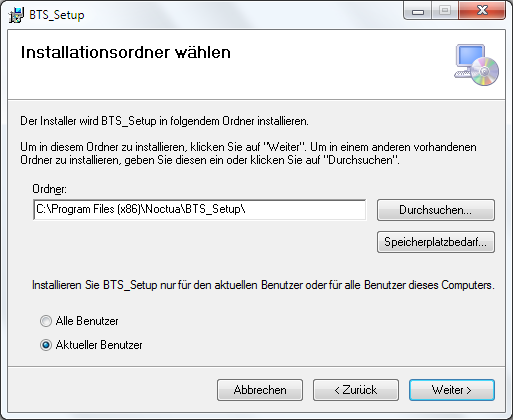
\includegraphics[width=1\textwidth]{images/btsinstall1.png}
\caption{Konfigurieren der Installtion}
\end{figure}
Nach der korrekten Konfiguration des Setups kann die Installtion gestartet werden.
\begin{figure}[H]
\centering
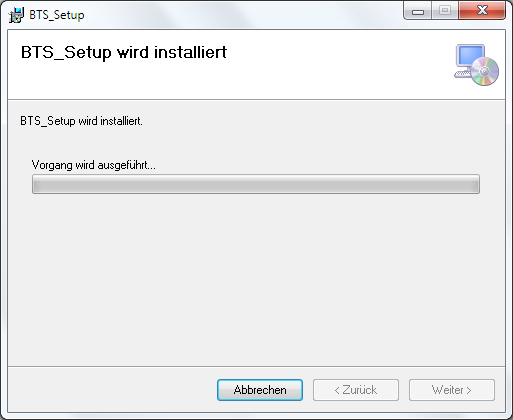
\includegraphics[width=1\textwidth]{images/btsinstall2.png}
\caption{Installationsvorgang}
\end{figure}
Nach diesem Vorgang ist die Backtesting-Software vollständig installiert und ausführbar.
%!TEX root=../Benutzerhandbuch.tex
\section{Programm}
%!TEX root=../../Benutzerhandbuch.tex
\section{Schreiben eines Algorithmus}
Um die Software zu bedienen wird ein in \gls{F-Sharp} geschriebener Algorithmus benötigt. Dieser muss als \gls{DLL}-Datei zur Laufzeit in die Software eingebunden werden. Eine solche Datei wird mittels Microsoft Visual Studio erzeugt werden, damit die Software funktionieren soll. \\
Folgende Eigenschaften muss die Datei erfüllen:
\begin{itemize}
	\item Name der Methode: startCalculation
	\item Übergabeparameter 1: eine Liste aller historischen Daten 
	\item Übergabeparameter 2: eine Liste der Signale für die Entscheidungen (bei Übergabe ist diese Liste leer)
\end{itemize}
Mit dem Rückgabewert der Methode wird nicht gearbeitet, sondern mit der vom Algorithmus verarbeiteten Signalliste.

\begin{lstlisting}[caption=Dateityp des 1. Übergabeparameters]{prices}
System.Collections.Generic.List<System.Tuple
<System.DateTime,decimal,decimal,decimal,decimal>>
\end{lstlisting}
\begin{lstlisting}[caption=Dateityp des 2. Übergabeparameters]{signals}
System.Collections.Generic.List<int>
\end{lstlisting}
Außerdem muss sich der Algorithmus im Namespace  "`Algorithm"' und im Modul "`DecisionCalculator"' befinden.
\subsection{Erzeugen eines Algorithmus-Files}
Öffnen Sie Microsoft Visual Studio und erzeugen sie ein neues Projekt.\\
\begin{figure}[H]
\centering
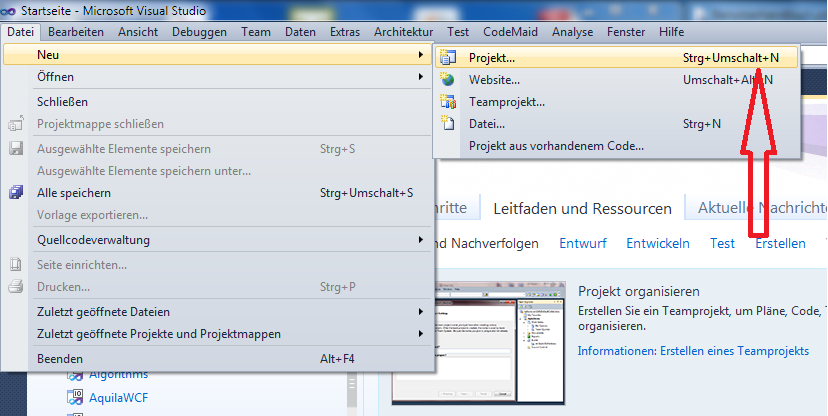
\includegraphics[width=1\textwidth]{images/newProject.png}
\caption{Erzeugen eines neuen Projekts}
\end{figure} 
\newpage
Erstellen Sie es als \gls{F-Sharp}-Bibliothek.
\begin{figure}[H]
\centering
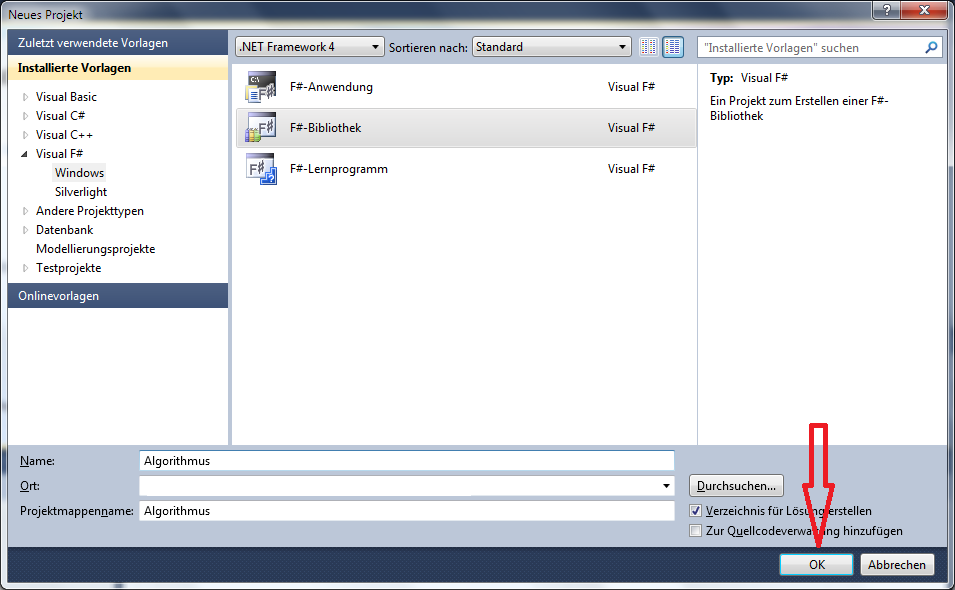
\includegraphics[width=1\textwidth]{images/createProject.png}
\caption{Erstellen Sie es als \gls{F-Sharp}-Bibliothek}
\end{figure}
Halten Sie sich an die, im Kapitel "`Schreiben eines Algorithmus"', genannten Richtlinien und implementieren die Methode startCalculation und kompilieren sie das Projekt.
\begin{figure}[H]
\centering
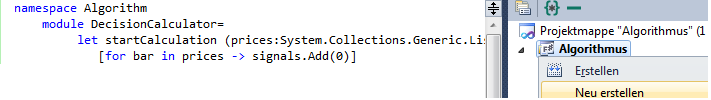
\includegraphics[width=1\textwidth]{images/makeFs.png}
\caption{Kompilieren des Projekts}
\end{figure}
\clearpage
\subsection{Entscheidungen}
Folgende Entscheidungen sind zulässig:
\begin{center}
\begin{tabular}{ |  p{1cm} | p{8cm} |}
\hline 
3 & starkes Kaufssignal \\ \hline
2 &   mittleres Kaufssignal \\ \hline
1 &  schwaches Kaufssignal\\ \hline
0 &  Alle Bestände werden gekauft oder verkauft\\ \hline
-1 &  schwaches Verkaufssignal\\ \hline
-2 &  mittleres Verkaufssignal\\ \hline
-3 &  starkes Verkaufssignal\\ \hline
\end{tabular}
\end{center}

%!TEX root=../../Benutzerhandbuch.tex
\section{Historische Daten}

Um einen Algorithmus mit der \gls{BTS} testen zu k�nnen, m�ssen auch noch historische Aktien-Preisdaten in die Software eingebunden werden, �ber die der Algorithmus getestet wird. Diese k�nnen in Form einer \gls{CSV}-Datei gespeichert und ihr Pfad in der \gls{BTS} angegeben werden. Dabei wurde ein sehr weit verbreitetes Format benutzt, das bspw. auch jegliche Software des renomierten Aktiendatenbereitstellungs-Unternehmens eSignal exportieren kann. Au�erdem werden in dieser Datei die historischen Daten in Form von \glspl{Bar} �ber einen bestimmten Zeitraum (z.B. Daily-\gls{Bar} oder Minute-\gls{Bar}) erwartet und nicht als einzelne Preiswerte. Das Format sieht in etwa so aus:

\begin{lstlisting}[caption=Aufbau der \gls{CSV}-Datei]{csv}
Bar,Date,Time,Open,High,Low,Close
1,01/02/90,00:00,8.8125,9.375, 8.75,9.3125
2,01/03/90,00:00,9.375, 9.50,9.375,9.375
3,01/04/90,00:00,9.375,9.6875,9.3125,9.40625
...
\end{lstlisting}

Zuerst steht also die Nummer des Bars, die allerdings nicht ber�cksichtigt wird. Darauf folgt das Datum in der Form \inline{MM/DD/YY} und die Uhrzeit in der Form \inline{hh:mm}. Zu guter Letzt kommen nun nur noch die Werte Open, High, Low und Close des \glspl{Bar}. Diese Datei kann nahezu unendlich lange gemacht werden, es k�nnen also nahezu unendlich viele Bars nach unten hin erg�nzt werden. Die erste Zeile der Datei wird im Allgemeinen nicht ber�cksichtigt, da sie meist die �berschriften enth�lt. Sollte sich in der ersten Zeile also ein Bar befinden, wird dieser ebenfalls ignoriert.
%!TEX root=../../Benutzerhandbuch.tex
\section{Backtestingsoftware}

Die \gls{BTS} ist nun also die Kernsoftware, mit der die Algorithmen �ber Daten-Files getestet werden k�nnen. Dazu sollten zuerst die allgemeinen Einstellungen get�tigt werden. Diese befinden sich im Settings-Tab unter ''Orders'' und sehen so aus:

\begin{figure}[H]
\centering
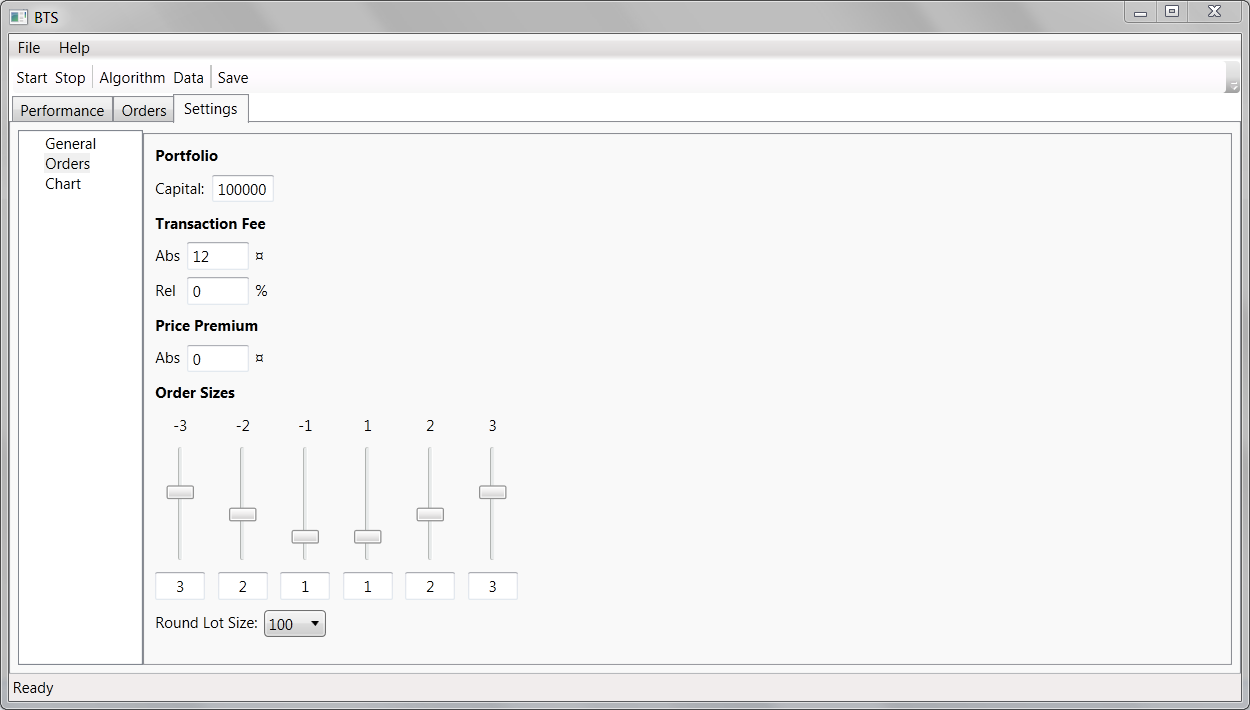
\includegraphics[width=1\textwidth]{images/btsordersettings.png}
\caption{Order-Settings der \gls{BTS}}
\end{figure}

Hier kann zuerst das gew�nschte Kapital eingestellt werden, dessen Handel die \gls{BTS} simulieren soll. Danach k�nnen Transaktionsgeb�hren absolut oder relativ, ein Preisaufschlag f�r K�ufe und die Order-Gr��en eingestellt werden. Die Order-Gr��en geben an, wie viele Round Lots bei einem Signal von -3 bis +3 gekauft/verkauft werden sollen. Ein Round Lot ist hierbei die kleinste �ber einen Online-Broker erwerbbare Menge an Aktien, die ebenfalls variieren und daher eingestellt werden kann.\\ \\

Auf der Seite darunter, der ''Chart''-Seite, k�nnen verschiedene Indikatoren aus der Combobox ausgew�hlt und hinzugef�gt werden, die dann nach der Performancemessung in die Grafik im Orders-Tab eingezeichnet werden. Hier k�nnen au�erdem f�r jeden Indikator die entsprechend notwendigen Parameter und Farben ausgew�hlt werden.

\begin{figure}[H]
\centering
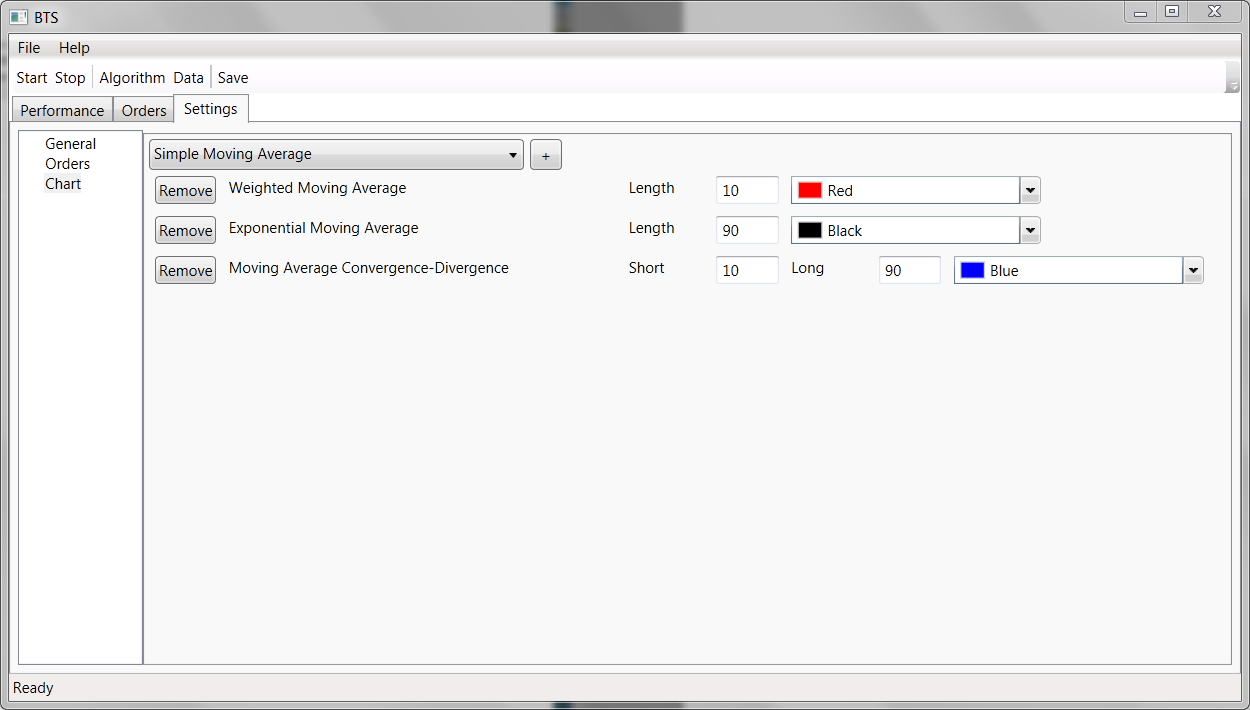
\includegraphics[width=1\textwidth]{images/btschartsettings.png}
\caption{Chart-Settings der \gls{BTS}}
\end{figure}

Weiters k�nnen nun unter der Seite ''General'' die eigentlich wichtigsten Informationen festgelegt werden. Diese sind die Pfade zur Algorithmus- und zur Daten-Datei, die in den vorherigen Punkten erl�utert wurden. Diese Pfade k�nnen �brigens auch durch den ''Algorithm''- und den ''Data''-Button in der Men�leiste hinzugef�gt werden. Darunter kann noch eine Zeitspanne ausgew�hlt werden. Der Algorithmus wird dann nur �ber alle Daten getestet, die im Daten-File im gew�hlten Zeitraum vorkommen.

\begin{figure}[H]
\centering
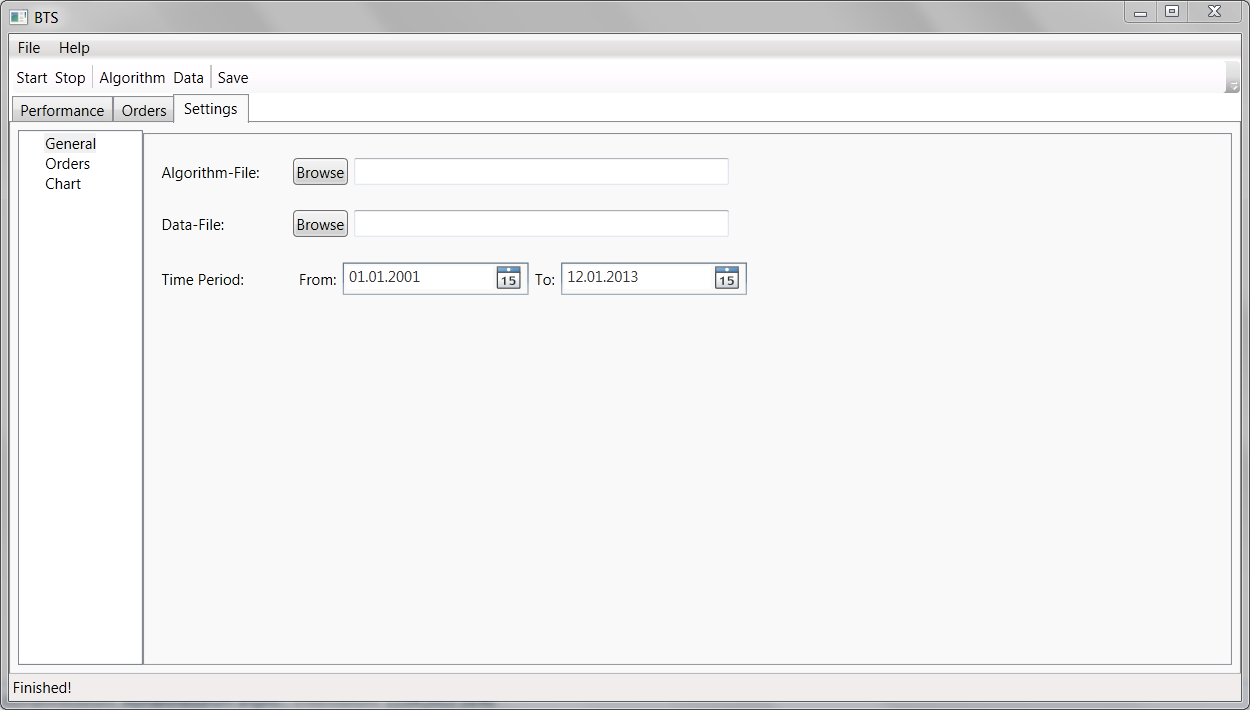
\includegraphics[width=1\textwidth]{images/btsgeneralsettings.png}
\caption{General-Settings der \gls{BTS}}
\end{figure}

Nachdem alle Einstellungen getroffen wurden, kann der Test gestartet werden.

\begin{figure}[H]
\centering
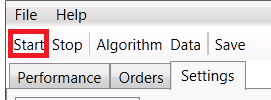
\includegraphics[width=0.6\textwidth]{images/btsstart.png}
\caption{Start-Button der \gls{BTS}}
\end{figure}

Anschlie�end werden auf dem Performance-Tab der \gls{BTS} die allgemeinen Performance-Daten des Algorithmus �ber das spezifizierte Daten-File ausgegeben. N�here Erkl�rungen zu diesen Werten k�nnen durch Halten der Maus �ber einen der Texte als Tooltip angezeigt werden.

\begin{figure}[H]
\centering
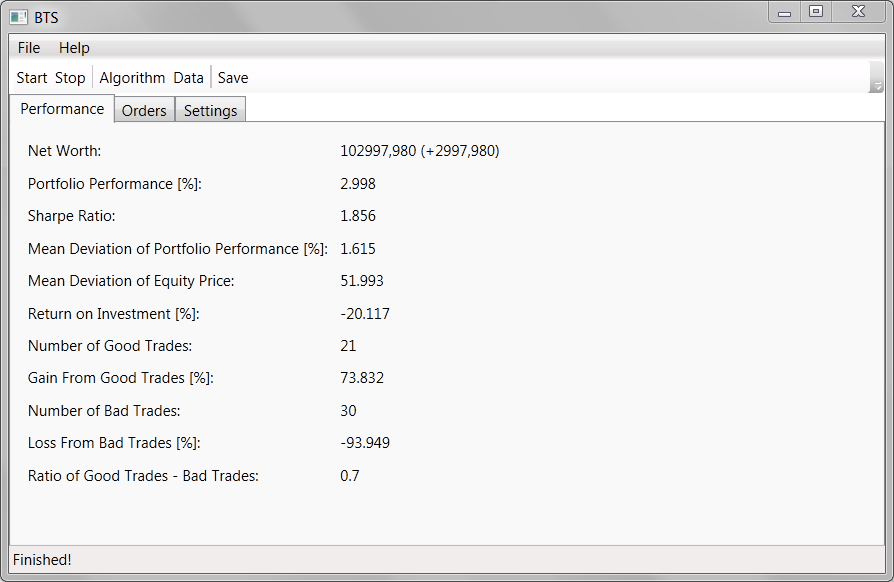
\includegraphics[width=1\textwidth]{images/btsperformance.png}
\caption{Start-Button der \gls{BTS}}
\end{figure}

Die meisten Informationen �ber den Verlauf des Tests k�nnen nun auf dem Orders-Tab gefunden werden. Hier wird zuerst oben ein Chart der Aktien-Preisdaten mit allen gew�hlten Indikatoren angezeigt. Durch Rechtsklick mit der Maus kann im Chart hinausgezoomt und mit der linken Maustaste hineingezoomt werden. Die Pfeile im Chart zeigen an, zu welchen Zeitpunkten der Algorithmus unter reellen Bedingungen �ber den gew�hlten Zeitabschnitt Signale ausgegeben h�tte. Die unterschiedlichen Farben und Farbschattierungen zeigen dabei ein Kauf- (Gr�n) oder ein Verkauf-Signal (Rot) und dessen St�rke an.\\
In der unteren H�lte des Bildschirms wird zu jedem dieser Signale ausgegeben welchen Effekt das jeweilige Signal auf das Kapital h�tte und welcher Gewinn oder Verlust dadurch zum damaligen Preis entstanden w�re. Position bzw. der Transaction Price geben dabei an, wieviele Round Lots durch dieses Signal gekauft worden w�ren und wieviel die Umsetzung des Signals kosten w�rde. Gain/Loss bezieht sich auf die prozentuelle Ver�nderung des Investitionskapitals der expliziten Order und Portfolio Performance auf die prozentuelle bzw. absolute Ver�nderung des gesamten gew�hlten Kapitals. All diese Werte werden auch kumulativ, also aufaddiert, angezeigt. 

\begin{figure}[H]
\centering
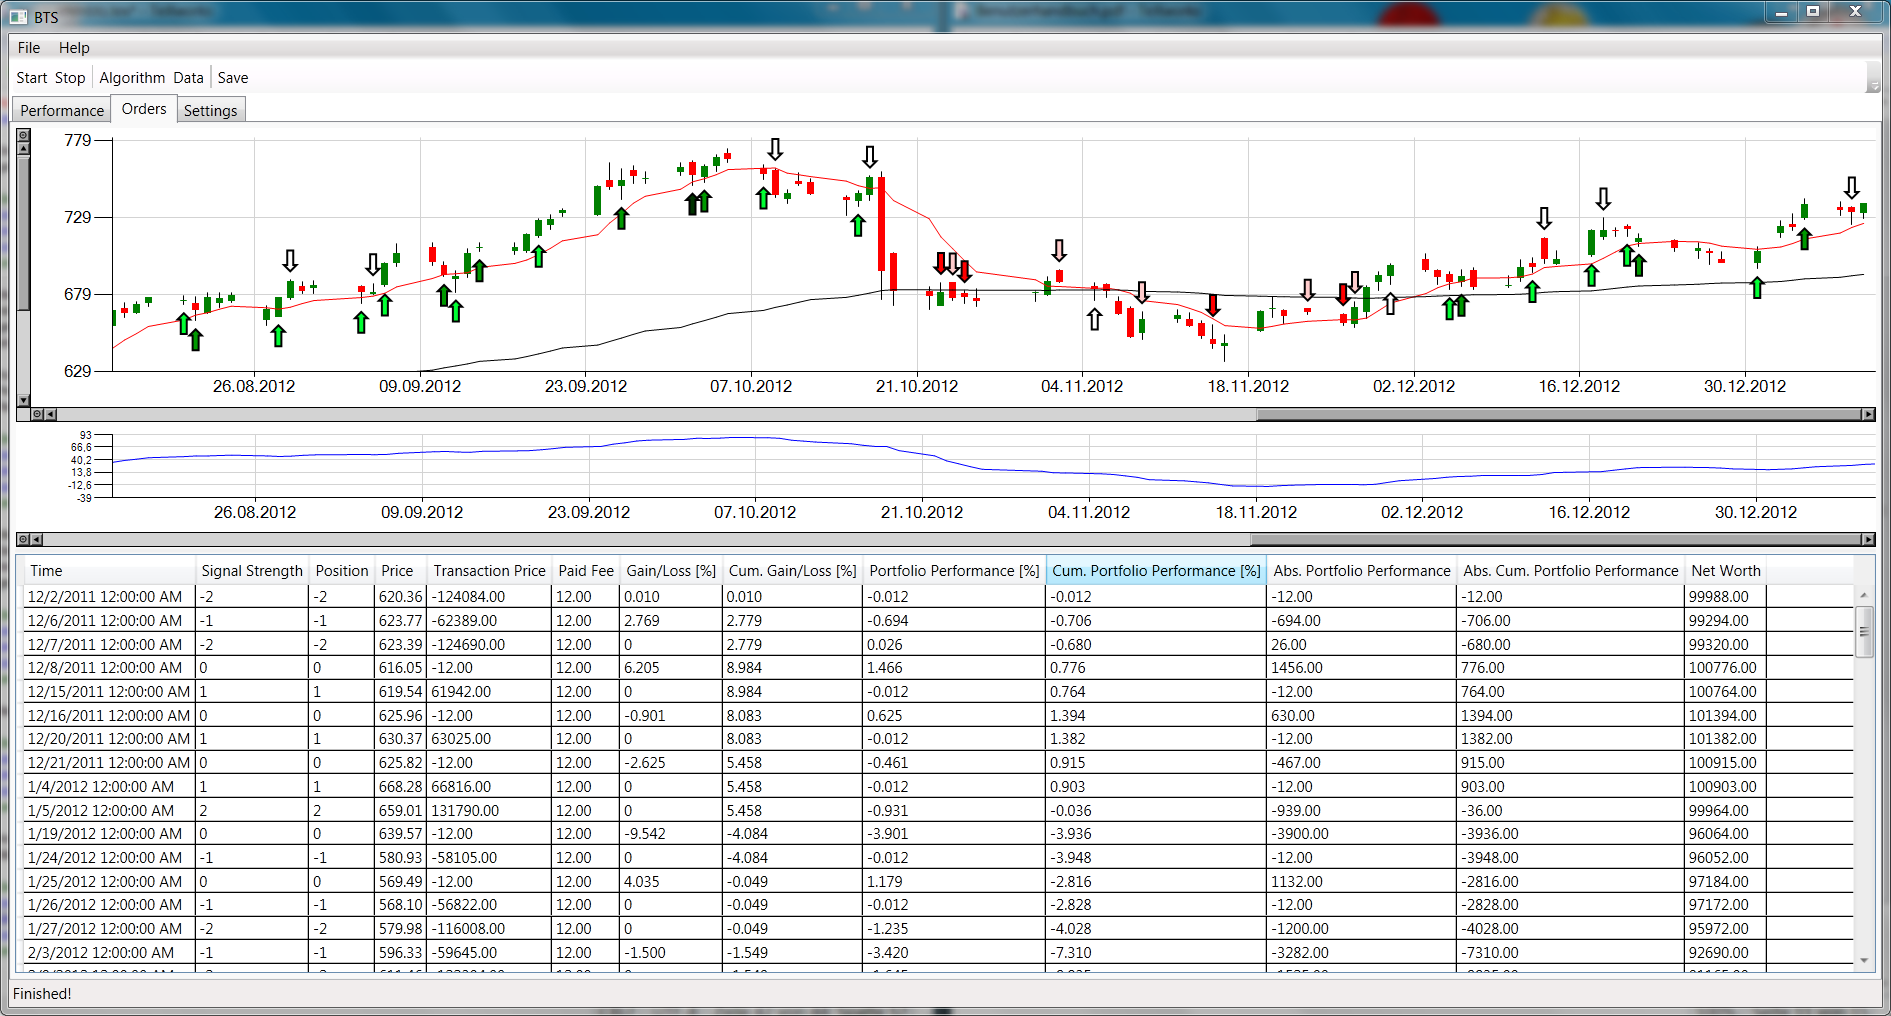
\includegraphics[width=1\textwidth]{images/btsorders.png}
\caption{Start-Button der \gls{BTS}}
\end{figure}

Zu guter Letzt k�nnen unter ''File'' -> ''Export'' die berechneten Performance-Daten lesbar als Text-File (.txt) exportiert werden. Au�erdem kann der aktuelle Zustand der \gls{BTS} inklusive aller Settings und berechneter Daten au�er der Charts (da sonst die Aktiendaten mitgespeichert werden m�ssten) gespeichert und zu einem sp�teren Zeitpunkt erneut geladen werden.
%!TEX root=../Benutzerhandbuch.tex
\chapter{Minimale Systemvoraussetzungen}
Folgende Vorraussetzungen m�ssen vom System erf�llt werden:\\
\textbf{Hardwareanforderungen}
\begin{center}
\begin{tabular}{ | l | c |}\hline 
Prozessor & 1 GHz \\ \hline
RAM & 512 MB \\ \hline
Festplattenspeicher (32 Bit) & 850 MB \\ \hline
Festplattenspeicher (64 Bit) & 2 GB \\ \hline
\end{tabular}
\end{center}
\textbf{Betriebssystemanforderungen} \\
Unterst�tzte Clientbetriebssysteme sind:
\begin{itemize}
\item Windows 8 (32-Bit- und 64-Bit-Editionen)
\item Windows 7 (32-Bit- und 64-Bit-Editionen)
\item Windows Vista (32-Bit- und 64-Bit-Editionen)
\end{itemize}

%\begin{landscape}

\chapter{Zeitaufzeichnungen}

\begin{figure}
	\centering
		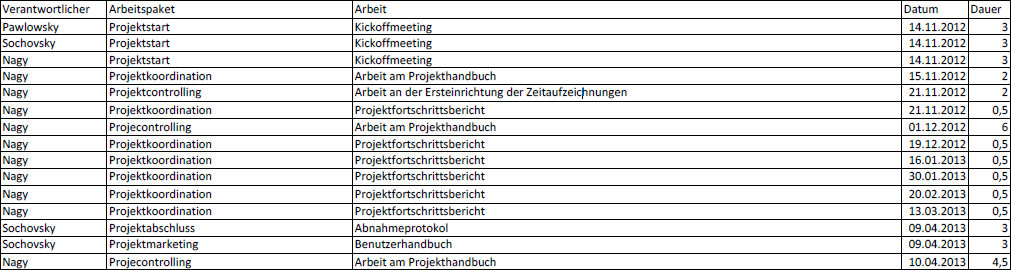
\includegraphics[width=1\textheight, angle=90]{graphics/appendix/projektmanagement.PNG}
	\caption{Projektmanagement}
\end{figure}

\begin{figure}
	\centering
		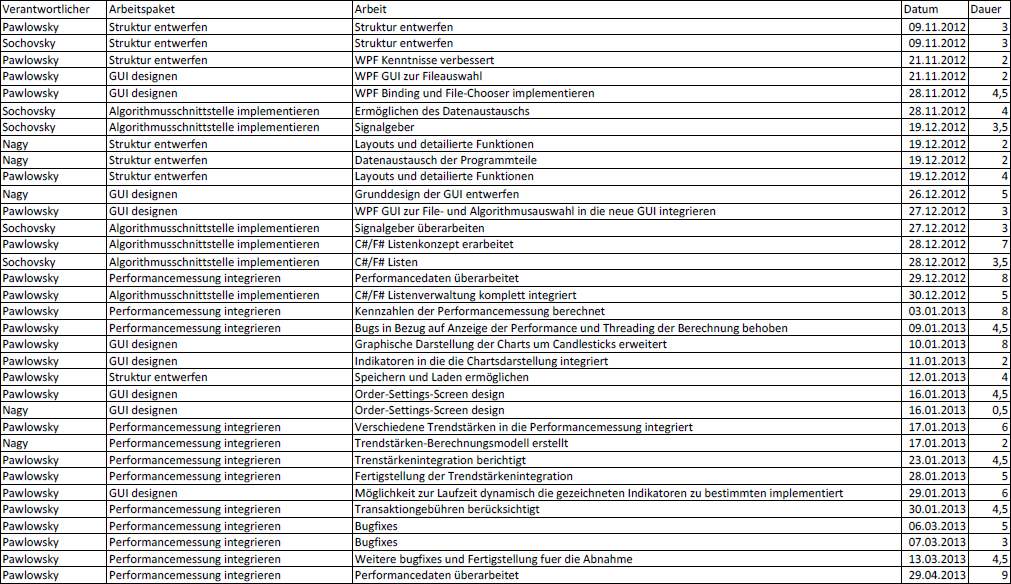
\includegraphics[width=1.0\textheight, angle=90]{graphics/appendix/backtestingsoftware.PNG}
	\caption{Backtesting-Software}
\end{figure}

\begin{figure}
	\centering
		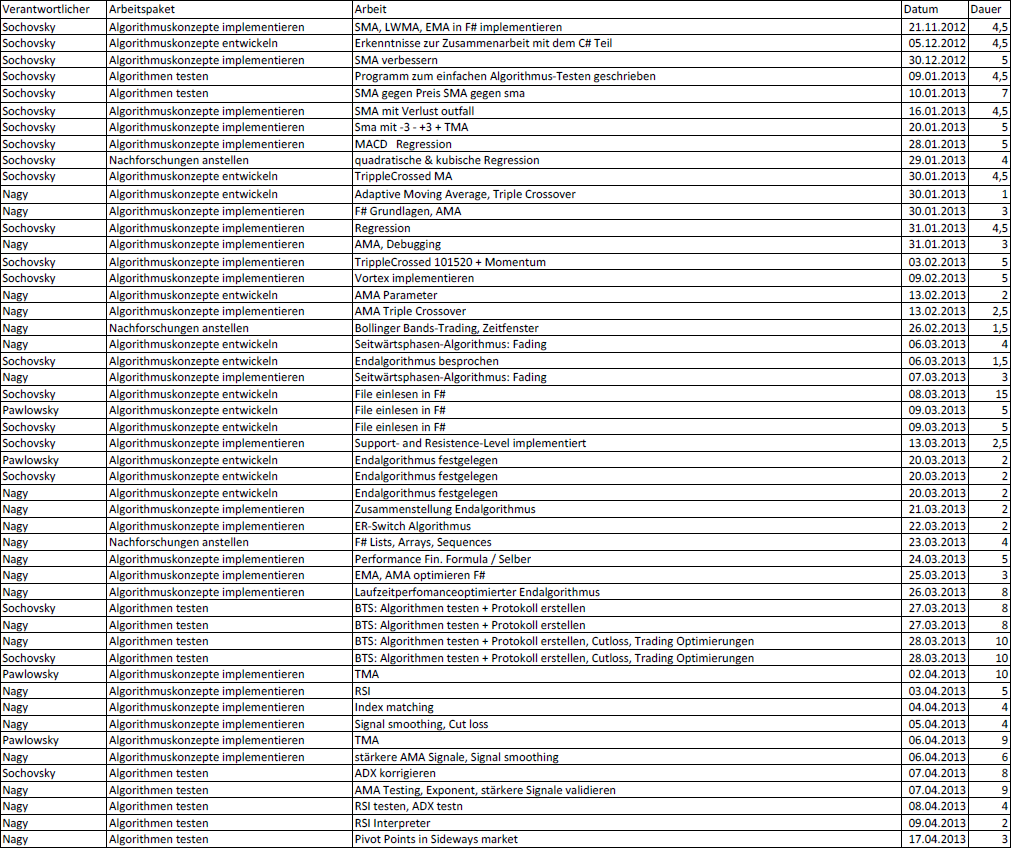
\includegraphics[width=1.0\textheight, angle=90]{graphics/appendix/algorithmus.PNG}
	\caption{Algorithmus}
\end{figure}

\begin{figure}
	\centering
		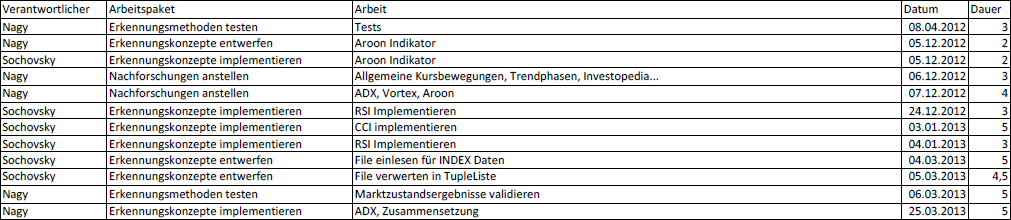
\includegraphics[width=1.0\textheight, angle=90]{graphics/appendix/marktzustandserkennung.PNG}
	\caption{Marktzustandserkennung}
\end{figure}

\begin{figure}
	\centering
		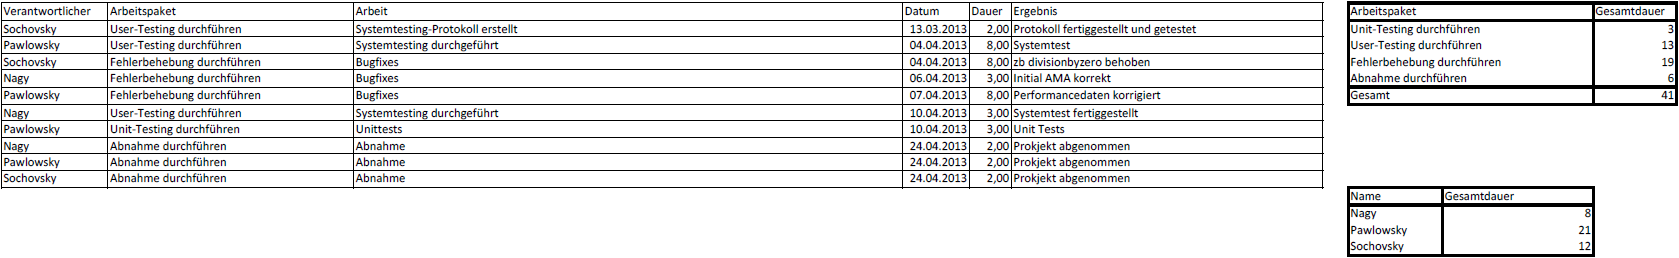
\includegraphics[width=1.0\textheight, angle=90]{graphics/appendix/testingabschluss.PNG}
	\caption{Testing \& Abschluss}
\end{figure}

%\end{landscape}%
\printglossary[type=\acronymtype]
\end{appendix}


\nomenclature[aa]{$t$}{time}
\nomenclature[bb]{$t_0$}{reference time}
\nomenclature[aa]{$m$}{mass}
\nomenclature[aa]{$\rho$}{mass density}

\markboth{\nomname}{\nomname}%
\addcontentsline{toc}{chapter}{\numberline{}\nomname}%
\printnomenclature

% Use of the sorted IEEE style, with changes:
% "dashification" was disabled


\cleardoublepage

% IEEE Style
\bibliographystyle{sty/IEEEtranS}

% GATHER
%\input "literatur/bib.bib"
\phantomsection{}
\addcontentsline{toc}{chapter}{\bibname}
\pagestyle{myheadings}\markboth{\bibname}{\bibname}
\bibliography{tex/bib_file}

%%% generate index
%\clearpage%
%\markboth{\indexname}{\indexname}%
%\printindex%
%\addcontentsline{toc}{chapter}{\numberline{}\indexname}%

%% include affidavit
\thispagestyle{empty}
\vspace*{2cm}
\begin{center}
{\bf \sf \huge Erkl{\"a}rung}
\end{center}
{\sf \vspace{1cm} Hiermit erkl{\"a}ren wir, dass die vorliegende
Arbeit ohne unzul{\"a}ssige Hilfe Dritter und ohne Benutzung
anderer als der angegebenen Hilfsmittel angefertigt wurde. Die aus
anderen Quellen oder indirekt �bernommenen Daten und Konzepte sind
unter Angabe der Quelle gekennzeichnet.

Die Arbeit wurde bisher weder im In- noch im Ausland in gleicher
oder in {\"a}hnlicher Form in anderen Pr{\"u}fungsverfahren
vorgelegt.
\\[1.5cm]
Wien, im \monthdis
\\[2cm]
Name1
\\[2cm]
Name2
\\[2cm]
Name3
\\[2cm]
Name4
\\[2cm]
}%end sf
%



\end{document}
%%%%%%%%%%%%%%%%%%%%%%%%%%%%%%%%%%%%%%%%%%%%%%%%%%%%%%%%%%%%%%%%%%%%%%%%%%%%%%%%%%%%%%%%%%%%%%%%%%%
%%%%%%%%%%%%%%%%%%%%%%%%%%%%%%%%%%%%%%%%%% End Dokument %%%%%%%%%%%%%%%%%%%%%%%%%%%%%%%%%%%%%%%%%%%
%%%%%%%%%%%%%%%%%%%%%%%%%%%%%%%%%%%%%%%%%%%%%%%%%%%%%%%%%%%%%%%%%%%%%%%%%%%%%%%%%%%%%%%%%%%%%%%%%%%
